%TODO select duplex for printing
%\documentclass[11pt,a4paper,oneside]{report}             % Single-side
\documentclass[11pt,onehalfspacing,a4paper,twoside,openright]{report}  % Duplex
 
\usepackage{ifxetex}
\ifxetex
  \usepackage{fontspec}
\else
  \usepackage[T1]{fontenc}
  \usepackage[utf8]{inputenc}
  \usepackage{lmodern}
\fi

\usepackage[bitstream-charter]{mathdesign}

\usepackage[english,magyar]{babel} % Alapértelmezés szerint utoljára definiált nyelv lesz aktív, de később külön beállítjuk az aktív nyelvet.

\usepackage{cmap}
\usepackage{amsfonts,amsmath} % Mathematical symbols.
\usepackage[ruled,boxed,resetcount,linesnumbered]{algorithm2e} % For pseudocodes.
\usepackage{booktabs} % For publication quality tables for LaTeX
\usepackage{graphicx}

%\usepackage{fancyhdr}
%\usepackage{lastpage}

\usepackage{anysize}
\usepackage{sectsty}
\usepackage{setspace}  % Ettol a tablazatok, abrak, labjegyzetek maradnak 1-es sorkozzel!


\usepackage{color}
\usepackage{listings} % For source code snippets.

\usepackage[amsmath,thmmarks]{ntheorem} % Theorem-like environments.

\usepackage[hang]{caption}

\newcommand{\selecthungarian}{
	\selectlanguage{magyar}
	\setlength{\parindent}{0em} % angol nyelvű dokumentumokban jellemző
	\setlength{\parskip}{0.5em} % angol nyelvű dokumentumokban jellemző
	\frenchspacing
}

\newcommand{\selectenglish}{
	\selectlanguage{english}
%	\setlength{\parindent}{2em} % angol nyelvű dokumentumokban jellemző
%	\setlength{\parskip}{0em}   % angol nyelvű dokumentumokban jellemző
	\setlength{\parindent}{0em} % angol nyelvű dokumentumokban jellemző
	\setlength{\parskip}{0.5em} % angol nyelvű dokumentumokban jellemző
	\nonfrenchspacing
	\renewcommand{\figureautorefname}{Figure}
	\renewcommand{\tableautorefname}{Table}
	\renewcommand{\partautorefname}{Part}
	\renewcommand{\chapterautorefname}{Chapter}
	\renewcommand{\sectionautorefname}{Section}
	\renewcommand{\subsectionautorefname}{Section}
	\renewcommand{\subsubsectionautorefname}{Section}
	\renewcommand{\algorithmautorefname}{Algorithm}
}

\usepackage{afterpage} 

\usepackage{algorithm2e}

\usepackage{pdfpages}

\usepackage{hyperref} % For hyperlinks in the generated document.

%\usepackage{cleveref} % For hyperlinks in the generated document.

%\renewcommand*{\listalgorithmcfname}{List of Heuristics}
%\renewcommand*{\algorithmcfname}{Heuristic}
\usepackage{subfig}



\newcommand{\vikszerzoVezeteknev}{Búr}
\newcommand{\vikszerzoKeresztnev}{Márton}
\newcommand{\vikkonzulensA}{Dr.~Ákos Horváth} % Első konzulens neve
\newcommand{\vikkonzulensB}{Zoltán Ujhelyi} % Második konzulens neve; hagyd üresen, ha egy konzulensed van.
\newcommand{\vikcim}{A general purpose local search-based pattern matching framework} % Cím
\newcommand{\viktanszek}{\bmemit} % Tanszék
\newcommand{\vikdoktipus}{\msc} % Dokumentum típusa (\bsc, \msc)

%--------------------------------------------------------------------------------------
% TDK-specifikus változók
%--------------------------------------------------------------------------------------
\newcommand{\tdkszerzoB}{Második Szerző} % Második szerző neve; hagyd üresen, ha egyedül í­rtad a TDK-t.
\newcommand{\tdkev}{2014} % A dolgozat írásának éve (pl. "2014") (Ez OTDK-nál eltérhet az aktuális évtől.)

% További adatok az OTDK címlaphoz (BME-s TDK-hoz nem kell kitölteni)
\newcommand{\tdkevfolyamA}{IV} % Első szerző évfolyama, római számmal (pl. IV).
\newcommand{\tdkevfolyamB}{III} % Második szerző évfolyama, római számmal (pl. III).
\newcommand{\tdkkonzulensbeosztasA}{egyetemi tanár} % Első konzulens beosztása (pl. egyetemi docens)
\newcommand{\tdkkonzulensbeosztasB}{doktorandusz} % Második konzulens beosztása (pl. egyetemi docens)

\newcommand{\szerzoMeta}{\vikszerzoVezeteknev{} \vikszerzoKeresztnev} % egy szerző esetén
%\newcommand{\szerzoMeta}{\vikszerzoVezeteknev{} \vikszerzoKeresztnev, \tdkszerzoB} % két szerző esetén

%%--------------------------------------------------------------------------------------
% Elnevezések
%--------------------------------------------------------------------------------------
\newcommand{\bme}{Budapesti Műszaki és Gazdaságtudományi Egyetem}
\newcommand{\vik}{Villamosmérnöki és Informatikai Kar}

\newcommand{\bmemit}{Méréstechnika és Információs Rendszerek Tanszék}

\newcommand{\keszitette}{Készítette}
\newcommand{\konzulens}{Konzulens}

\newcommand{\bsc}{Szakdolgozat}
\newcommand{\msc}{Diplomaterv}

\newcommand{\pelda}{Példa}
\newcommand{\definicio}{Definíció}
\newcommand{\tetel}{Tétel}

\newcommand{\bevezeto}{Bevezető}
\newcommand{\koszonetnyilvanitas}{Köszönetnyilvánítás}
\newcommand{\abrakjegyzeke}{Ábrák jegyzéke}
\newcommand{\tablazatokjegyzeke}{Táblázatok jegyzéke}
\newcommand{\irodalomjegyzek}{Irodalomjegyzék}
\newcommand{\fuggelek}{Függelék}

\newcommand{\szerzo}{\vikszerzoVezeteknev{} \vikszerzoKeresztnev}

\newcommand{\selectthesislanguage}{\selecthungarian}

\bibliographystyle{huplain}

\def\lstlistingname{lista}

\newcommand{\appendixnumber}{6}  % a fofejezet-szamlalo az angol ABC 6. betuje (F) lesz
  % Beállítások magyar nyelvű dolgozathoz
%--------------------------------------------------------------------------------------
% Elnevezések
%--------------------------------------------------------------------------------------
\newcommand{\bme}{Budapest University of Technology and Economics}
\newcommand{\vik}{Faculty of Electrical Engineering and Informatics}

\newcommand{\bmemit}{Department of Measurement and Information Systems}

\newcommand{\keszitette}{Author}
\newcommand{\konzulens}{Advisor}

\newcommand{\bsc}{Bachelor's Thesis}
\newcommand{\msc}{Master's Thesis}

\newcommand{\pelda}{Example}
\newcommand{\definicio}{Definition}
\newcommand{\tetel}{Theorem}

\newcommand{\bevezeto}{Introduction}
\newcommand{\koszonetnyilvanitas}{Acknowledgements}
\newcommand{\abrakjegyzeke}{List of Figures}
\newcommand{\tablazatokjegyzeke}{List of Tables}
\newcommand{\irodalomjegyzek}{Bibliography}
\newcommand{\fuggelek}{Appendix}

\newcommand{\szerzo}{\vikszerzoKeresztnev{} \vikszerzoVezeteknev}

\newcommand{\selectthesislanguage}{\selectenglish}

\bibliographystyle{plain}

\newcommand{\ie}{i.e.\@\xspace}
\newcommand{\Ie}{I.e.\@\xspace}
\newcommand{\eg}{e.g.\@\xspace}
\newcommand{\Eg}{E.g.\@\xspace}
\newcommand{\etal}{et al.\@\xspace}
\newcommand{\etc}{etc.\@\xspace}

\renewcommand{\figureautorefname}{Figure}
\renewcommand{\tableautorefname}{Table}
\renewcommand{\partautorefname}{Part}
\renewcommand{\chapterautorefname}{Chapter}
\renewcommand{\sectionautorefname}{Section}
\renewcommand{\subsectionautorefname}{Section}
\renewcommand{\subsubsectionautorefname}{Section}

\newcommand{\appendixnumber}{1}  % a fofejezet-szamlalo az angol ABC 1. betuje (A) lesz
 % Settings for English documents

%--------------------------------------------------------------------------------------
% Page layout setup
%--------------------------------------------------------------------------------------
% we need to redefine the pagestyle plain
% another possibility is to use the body of this command without \fancypagestyle
% and use \pagestyle{fancy} but in that case the special pages
% (like the ToC, the References, and the Chapter pages)remain in plane style

\pagestyle{plain}
\marginsize{35mm}{25mm}{15mm}{15mm}

\setcounter{secnumdepth}{0}
\sectionfont{\large\upshape\bfseries}
\setcounter{secnumdepth}{2}

\sloppy % Margón túllógó sorok tiltása.
\widowpenalty=10000 \clubpenalty=10000 %A fattyú- és árvasorok elkerülése
\def\hyph{-\penalty0\hskip0pt\relax} % Kötőjeles szavak elválasztásának engedélyezése


%--------------------------------------------------------------------------------------
% Setup hyperref package
%--------------------------------------------------------------------------------------
\hypersetup{
    bookmarks=true,            % show bookmarks bar?
    unicode=false,              % non-Latin characters in Acrobat's bookmarks
    pdftitle={\vikcim},        % title
    pdfauthor={\szerzoMeta},    % author
    pdfsubject={\vikdoktipus}, % subject of the document
    pdfcreator={\szerzoMeta},   % creator of the document
    pdfproducer={},    % producer of the document
    pdfkeywords={},    % list of keywords (separate then by comma)
    pdfnewwindow=true,         % links in new window
    colorlinks=true,           % false: boxed links; true: colored links
    linkcolor=black,           % color of internal links
    citecolor=black,           % color of links to bibliography
    filecolor=black,           % color of file links
    urlcolor=black             % color of external links
}


%--------------------------------------------------------------------------------------
% Set up listings
%--------------------------------------------------------------------------------------
\definecolor{lightgray}{rgb}{0.95,0.95,0.95}
\lstset{
	basicstyle=\scriptsize\ttfamily, % print whole listing small
	keywordstyle=\color{black}\bfseries, % bold black keywords
	identifierstyle=, % nothing happens
	commentstyle=\color{green}, % green comments
	stringstyle=\scriptsize,
	showstringspaces=false, % no special string spaces
	aboveskip=3pt,
	belowskip=3pt,
	backgroundcolor=\color{lightgray},
	columns=flexible,
	keepspaces=true,
	escapeinside={(*@}{@*)},
	captionpos=b,
	breaklines=true,
	frame=single,
	float=!ht,
	literate=*
		{á}{{\'a}}1	{é}{{\'e}}1	{í}{{\'i}}1	{ó}{{\'o}}1	{ö}{{\"o}}1	{ő}{{\H{o}}}1	{ú}{{\'u}}1	{ü}{{\"u}}1	{ű}{{\H{u}}}1
		{Á}{{\'A}}1	{É}{{\'E}}1	{Í}{{\'I}}1	{Ó}{{\'O}}1	{Ö}{{\"O}}1	{Ő}{{\H{O}}}1	{Ú}{{\'U}}1	{Ü}{{\"U}}1	{Ű}{{\H{U}}}1
}


%--------------------------------------------------------------------------------------
% Set up theorem-like environments
%--------------------------------------------------------------------------------------
% Using ntheorem package -- see http://www.math.washington.edu/tex-archive/macros/latex/contrib/ntheorem/ntheorem.pdf

\theoremstyle{plain}
\theoremseparator{.}
\newtheorem{example}{\pelda}

\theoremseparator{.}
%\theoremprework{\bigskip\hrule\medskip}
%\theorempostwork{\hrule\bigskip}
\theorembodyfont{\upshape}
\theoremsymbol{{\large \ensuremath{\centerdot}}}
\newtheorem{definition}{\definicio}

\theoremseparator{.}
%\theoremprework{\bigskip\hrule\medskip}
%\theorempostwork{\hrule\bigskip}
\newtheorem{theorem}{\tetel}


%--------------------------------------------------------------------------------------
% Some new commands and declarations
%--------------------------------------------------------------------------------------
\newcommand{\code}[1]{{\upshape\ttfamily\scriptsize\indent #1}}
\newcommand{\doi}[1]{DOI: \href{http://dx.doi.org/\detokenize{#1}}{\raggedright{\texttt{\detokenize{#1}}}}} % A hivatkozások közt így könnyebb DOI-t megadni.

\DeclareMathOperator*{\argmax}{arg\,max}
%\DeclareMathOperator*[1]{\floor}{arg\,max}
\DeclareMathOperator{\sign}{sgn}
\DeclareMathOperator{\rot}{rot}


%--------------------------------------------------------------------------------------
% Setup captions
%--------------------------------------------------------------------------------------
\captionsetup[figure]{
	width=.75\textwidth,
	aboveskip=10pt}

\renewcommand{\captionlabelfont}{\bf}
%\renewcommand{\captionfont}{\footnotesize\it}


%--------------------------------------------------------------------------------------
% Redefine reference style
%--------------------------------------------------------------------------------------
\newcommand{\figref}[1]{\ref{fig:#1}.}
\renewcommand{\eqref}[1]{(\ref{eq:#1})}
\newcommand{\listref}[1]{\ref{listing:#1}.}
\newcommand{\sectref}[1]{\ref{sect:#1}}
\newcommand{\tabref}[1]{\ref{tab:#1}.}


%--------------------------------------------------------------------------------------
% Hyphenation exceptions
%--------------------------------------------------------------------------------------
\hyphenation{Shakes-peare Mar-seilles ár-víz-tű-rő tü-kör-fú-ró-gép}


\author{\vikszerzo}
\title{\viktitle}


\usepackage{xcolor}
\usepackage{xspace}

% pattern colors
\definecolor{negcolor}{RGB}{223,49,35}
\definecolor{newcolor}{RGB}{43,183,47}
\definecolor{delcolor}{RGB}{59,66,161}

% listing colors
\definecolor{backgroundcolor}{HTML}{F5F5F5}
\definecolor{keywordcolor}{HTML}{295F94}
\definecolor{commentcolor}{HTML}{AD95AF}
\definecolor{stringcolor}{HTML}{317ECC}

\newcommand{\union}{\cup}
\newcommand{\intersection}{\cap}
\newcommand{\parentheses}[1]{\left(#1\right)}
\newcommand{\op}[2]{\mathrm{#1}\parentheses{#2}}
\newcommand{\naturaljoin}{\bowtie}
\newcommand{\antijoin}{\, \triangleright \,}
\newcommand{\iq}{\mbox{\textsc{IncQuery}}\xspace}
\newcommand{\iqpl}{\mbox{\textsc{IncQuery}} Pattern Language\xspace}
\newcommand{\iqd}{\mbox{\textsc{IncQuery-D}}\xspace}
\newcommand{\eiq}{\mbox{\textsc{EMF-IncQuery}}\xspace}
\newcommand{\emfapi}{\mbox{EMF API}\xspace}
\newcommand{\tb}{Train Benchmark\xspace}
\renewcommand{\ie}{i.e.,\@\xspace}
\renewcommand{\Ie}{I.e.,\@\xspace}
\renewcommand{\eg}{e.g.,\@\xspace}
\renewcommand{\Eg}{E.g.,\@\xspace}
\renewcommand{\etal}{et al.\@\xspace}
\renewcommand{\etc}{etc.\@\xspace}

% scenarios
\newcommand{\scenario}[1]{\textsf{#1}\xspace}
\newcommand{\batch}{\scenario{Batch}}
\newcommand{\inject}{\scenario{Inject}}
\newcommand{\repair}{\scenario{Repair}}

% phases 
\newcommand{\phase}[1]{\textsf{#1}\xspace}
\renewcommand{\read}{\phase{read}}
\renewcommand{\check}{\phase{check}}
\newcommand{\transformation}{\phase{transformation}}
\newcommand{\recheck}{\phase{recheck}}

\newcommand{\readandcheck}{\phase{\read and \check}}
\newcommand{\transformationandrecheck}{\phase{\transformation and \recheck}}
% queries
\newcommand{\query}[1]{\textsf{#1}\xspace}
\newcommand{\connectedsegments}{\query{Connected\-Segments}}
\newcommand{\poslength}{\query{PosLength}}
\newcommand{\routesensor}{\query{Route\-Sensor}}
\newcommand{\semaphoreneighbor}{\query{Semaphore\-Neighbor}}
\newcommand{\switchsensor}{\query{Switch\-Sensor}}
\newcommand{\switchset}{\query{SwitchSet}}

% table headers
\newcommand*{\theadswfirst}[1]{\multicolumn{1}{|c|}{\bfseries \begin{sideways}#1\end{sideways}}}
\newcommand*{\theadsw}[1]{\multicolumn{1}{c|}{\bfseries \begin{sideways}#1\end{sideways}}}
\newcommand*{\theadfirst}[1]{\multicolumn{1}{|c|}{\bfseries #1}}
\newcommand*{\thead}[1]{\multicolumn{1}{c|}{\bfseries #1}}

% for the hyperref package
\renewcommand{\sectionautorefname}{Section}
\renewcommand{\subsectionautorefname}{Section}
\renewcommand{\subsubsectionautorefname}{Section}

\newcommand{\patternscale}{0.23}
\newcommand{\yedscale}{0.50}
\newcommand{\ecorescale}{0.50}

\newcommand{\yes}{$\CIRCLE$\xspace}
\newcommand{\somewhat}{$\LEFTcircle$\xspace}
\newcommand{\no}{$\Circle$\xspace}

\newcommand{\forallqueries}[1]{\foreach \q in {ConnectedSegments,PosLength,RouteSensor,SemaphoreNeighbor,SwitchSensor,SwitchSet}{#1}}

\newcommand{\benchmarkresult}[3]{
\begin{figure*}[p]
	\centering
	\includegraphics[width=\textwidth]{benchmark-results/#1-#2}
	\caption{#3.}
	\label{fig:#1-#2}
\end{figure*}}

\newcommand{\patterngraphics}[1]{
	\centering
	\includegraphics[scale=\patternscale]{pattern-#1}
 	\caption{The \textsf{#1} pattern.}
 	\label{fig:pattern-#1}
}

\newcommand{\tbpattern}[1]{
\begin{figure}[H]
	\patterngraphics{#1}
\end{figure}}

\newcommand{\yedfigure}[2]{
\begin{figure}[H]
	\centering
	\includegraphics[scale=\yedscale]{yed/#1}
	\caption{#2.}
	\label{fig:#1}
\end{figure}}

\newcommand{\yedfigurelarge}[2]{
\begin{figure*}[htbp]
	\centering
	\includegraphics[scale=\yedscale]{yed/#1}
	\caption{#2.}
	\label{fig:#1}
\end{figure*}}

\newcommand{\tbtransformation}[2]{
\begin{figure}[H] 
	\centering
	\includegraphics[scale=\patternscale]{transformation-#1-#2}
 	\caption{The \textsf{#1} transformation for \textsf{#2}.}
 	\label{fig:transformation-#1-#2}
\end{figure}}

\lstset{
	numbers=left,
	numberstyle=\scriptsize\ttfamily,
	stepnumber=1,
	numbersep=5pt,
	%
	basicstyle=\scriptsize\ttfamily,
	backgroundcolor=\color{backgroundcolor},
	keywordstyle=\color{keywordcolor}\bfseries,
	commentstyle=\color{commentcolor},
	stringstyle=\color{stringcolor},
	identifierstyle=, % nothing happens
	%
	showstringspaces=false, % no special string spaces
	aboveskip=3pt,
	belowskip=3pt,
	columns=flexible,
	keepspaces=true,
	breaklines=true,	
	frameround=tttt,
	captionpos=b,
	tabsize=2,
	frame=tb,
	framerule=0pt,
	framexleftmargin=0.25em,
}

% languages

\lstdefinelanguage{iqpl}
{
	morekeywords={@QueryBasedFeature,@Constraint,count,pattern,package,neg,find,import,true,false,or,check,job,action,state,severity,location,message,oclIsKindOf,self,exists,includes,invariant,class},
	sensitive=true,
	morecomment=[l]{//},
	morecomment=[s]{/*}{*/},
	morestring=[b]{"},
}

\lstdefinelanguage{xtend}{
	morekeywords={class,for,def,val,var,cached,case,default,extension,false,import,JAVA,WORKFLOWSLOT,let,new,null,public,protected,private,create,switch,this,true,reexport,around,if,then,else,context,DEFAULT_NO_UPDATE_AND_DISAPPEAR,DEFAULT,APPEARED,DISAPPEARED,UPDATED,processor},
	morecomment=[l]{//},
	morecomment=[s]{/*}{*/},
	morestring=[b]",
	mathescape=true,
}

\lstdefinelanguage{sparql}{
	morekeywords={SELECT, DISTINCT, WHERE, OPTIONAL, FILTER, NOT, EXISTS, sameTerm, bound},
}

% listings

\newcommand{\listingiqpl}[2]
{
	\lstset{
		language=iqpl
	}
	\lstinputlisting[label=lst:#1, caption=#2.]{code/#1.eiq}
}

\newcommand{\listingjava}[2]{
	\lstset{
		language=Java
	}
	\lstinputlisting[label=lst:#1, caption=#2.]{code/#1.java}
}

\newcommand{\listingsparql}[2]{
	\lstset{
		language=sparql
	}
	\lstinputlisting[label=lst:query-#1, caption=#2.]{queries/#1.sparql}
}

\lstdefinelanguage{turtle}
{
	morekeywords={@prefix,@base,@forSome,@forAll,@keywords},
	morecomment=[l]{\#\ },
	morestring=[b]\"
}


\lstdefinelanguage{XML}
{
	morestring=[b]",
	morecomment=[s]{?}{?},
	morecomment=[s]{!--}{--},
	morekeywords={xmlns,version,xsi,xmi,graphml,graph},
}

\newcommand{\catchproblem}{\texttt{catchProblemFinder}\xspace}
\newcommand{\handlervar}{\texttt{handlerVariable}\xspace}
\newcommand{\baseindex}{\mbox{EMF-IncQuery} Base Index\xspace}
\newcommand{\screenshotscale}{0.74}
\newcommand{\stackedlines}[2]{\begin{tabular}{@{}c@{}}#1 \\ #2\end{tabular}}
\newcommand{\eobject}{\texttt{EObject}\xspace}

\newcommand{\todo}[1]{\textcolor{red}{\LARGE{TODO: #1}}\xspace}%
\newcommand{\Modeldriven}{Model-driven\xspace}
\newcommand{\modeldriven}{model-driven\xspace}
\newcommand{\matlab}{\textsc{Matlab}\xspace}
\newcommand{\simulink}{\textsc{Simulink}\xspace}
\newcommand{\matlabsimulink}{\textsc{Matlab-Simulink}\xspace}

\newcommand{\functionCall}[1]{\kern-0.25em(#1)}

%--------------------------------------------------------------------------------------
% Table of contents and the main text
%--------------------------------------------------------------------------------------
\begin{document}
\clearpage
%
\includepdf[pages=-]{pdfs/feladatkiiras.pdf}

\includepdf[pages=-]{pdfs/feladatkiiras-2oldal.pdf}

%~~~~~~~~~~~~~~~~~~~~~~~~~~~~~~~~~~~~~~~~~~~~~~~~~~~~~~~~~~~~~~~~~~~~~~~~~~~~~~~~~~~~~~
%\pagenumbering{gobble}
%\afterpage{\null\newpage}

\selectthesislanguage

%--------------------------------------------------------------------------------------
%	The title page
%--------------------------------------------------------------------------------------
\begin{titlepage}
\begin{center}

\includegraphics[width=60mm,keepaspectratio]{figures/pdfs/bme_logo.pdf}\\
\vspace{0.3cm}
\textbf{\bme}\\
\textmd{\vik}\\
\textmd{\viktanszek}\\[5cm]

\vspace{0.4cm}
{\huge \bfseries \vikcim}\\[0.8cm]
\vspace{0.5cm}
\textsc{\Large \vikdoktipus}\\[4cm]

{
	\renewcommand{\arraystretch}{0.85}
	\begin{tabular}{cc}
	 \makebox[7cm]{\emph{\keszitette}} & \makebox[7cm]{\emph{\konzulens}} \\ \noalign{\smallskip}
	 \makebox[7cm]{\szerzo} & \makebox[7cm]{\vikkonzulensA} \\
	  & \makebox[7cm]{\vikkonzulensB} \\
	\end{tabular}
}

\vfill
%{\large \today}
{\large December 11, 2015}
\end{center}
\end{titlepage}


		   % Szakdolgozat/Diplomaterv címlap
%%% TDK címlap
\begin{titlepage}
  \begin{center}  
  
\includegraphics[width=7cm]{./figures/bme_logo.pdf}
  \vspace{0.3cm}
  
  \bme \\
  \vik \\
  \viktanszek \\
  \vspace{5cm}
  
  \huge {\vikcim}
  \vspace{1.5cm}
  
  \large {\textbf{\vikdoktipus}}
  \vfill
    
  {\Large 
  	\keszitette: \\ \vspace{0.3cm}
  	\szerzo \\
	\tdkszerzoB \\
  	\vspace{1.5cm}
  	\konzulens: \\ \vspace{0.3cm}
  	\vikkonzulensA \\
  	\vikkonzulensB \\
  }
  
  \vspace{2cm}
  \large {\tdkev}
 \end{center}
\end{titlepage}
%% Címlap vége	% TDK címlap
%%% OTDK külső címlap
\begin{titlepage}
  	$\;$ 
	\vspace{5cm}
	
	\begin{center}
	\Huge
	\textbf{TDK-dolgozat}\let\thefootnote\relax\footnote{A dolgozat bemutatását a XXXXXXXXX  ``Lorem ipsum dolor sit amet'' című program támogatta.}
	\end{center}
	
	\vspace{13cm}
	
	\Large
	\hspace{8cm} \szerzo
	
	\hspace{8cm} \tdkszerzoB
	
	\hspace{8cm} \tdkev.
\end{titlepage}

\newpage
\thispagestyle{empty}


%% OTDK belső címlap
\begin{titlepage}
  \begin{center}  
  
\includegraphics[width=7cm]{./figures/bme_logo.pdf}
  \vspace{0.3cm}
  
  \bme \\
  \vik \\
  \viktanszek \\
  \vspace{3.5cm}
  
  \huge {\vikcim}
  \vspace{1.5cm}
  
  \large {\textbf{\vikdoktipus}}
  \vfill
    
  {\Large 
  	{\large \keszitette:} \\ \vspace{0.2cm}
  	\szerzo \\ \tdkevfolyamA. évfolyam \\
	\vspace{0.5cm}
	\tdkszerzoB \\ \tdkevfolyamB. évfolyam \\
  	\vspace{1.5cm}
  	{\large \konzulens:} \\ \vspace{0.2cm}
  	\vikkonzulensA,\\ \tdkkonzulensbeosztasA \\
  	\vspace{0.5cm}
  	\vikkonzulensB,\\ \tdkkonzulensbeosztasB \\
  }
  
  \vspace{2cm}
  \large {\tdkev.}
  
 \end{center}
\end{titlepage}   % OTDK címlap


% Table of Contents
%~~~~~~~~~~~~~~~~~~~~~~~~~~~~~~~~~~~~~~~~~~~~~~~~~~~~~~~~~~~~~~~~~~~~~~~~~~~~~~~~~~~~~~
\tableofcontents\vfill


% Declaration and Abstract
%~~~~~~~~~~~~~~~~~~~~~~~~~~~~~~~~~~~~~~~~~~~~~~~~~~~~~~~~~~~~~~~~~~~~~~~~~~~~~~~~~~~~~~
\selectlanguage{magyar}
\pagenumbering{gobble}


\clearpage\null\newpage
 
%--------------------------------------------------------------------------------------
% Nyilatkozat
%--------------------------------------------------------------------------------------
\begin{center}
\large
\textbf{HALLGATÓI NYILATKOZAT}\\
\end{center}

Alulírott \emph{\vikszerzoVezeteknev{} \vikszerzoKeresztnev}, szigorló hallgató kijelentem, hogy ezt a diplomatervet meg nem engedett segítség nélkül, saját magam készítettem, csak a megadott forrásokat (szakirodalom, eszközök stb.) használtam fel. Minden olyan részt, melyet szó szerint, vagy azonos értelemben, de átfogalmazva más forrásból átvettem, egyértelműen, a forrás megadásával megjelöltem.

Hozzájárulok, hogy a jelen munkám alapadatait (szerző(k), cím, angol és magyar nyelvű tartalmi kivonat, készítés éve, konzulens(ek) neve) a BME VIK nyilvánosan hozzáférhető elektronikus formában, a munka teljes szövegét pedig az egyetem belső hálózatán keresztül (vagy autentikált felhasználók számára) közzétegye. Kijelentem, hogy a benyújtott munka és annak elektronikus verziója megegyezik. Dékáni engedéllyel titkosított diplomatervek esetén a dolgozat szövege csak 3 év eltelte után válik hozzáférhetővé.

\begin{flushleft}
\vspace*{1cm}
Budapest, 2015. december 11. %\today
\end{flushleft}

\begin{flushright}
 \vspace*{1cm}
 \makebox[7cm]{\rule{6cm}{.4pt}}\\
 \makebox[7cm]{\emph{\vikszerzoVezeteknev{} \vikszerzoKeresztnev}}\\
 \makebox[7cm]{hallgató}
\end{flushright}
\thispagestyle{empty}

\vfill
\clearpage
\thispagestyle{empty} % an empty page

%\pagenumbering{gobble}
%\afterpage{\null\newpage}


\selectthesislanguage


\pagenumbering{gobble}
\afterpage{\null\newpage}

\pagenumbering{roman}
\setcounter{page}{1}

\selecthungarian

%----------------------------------------------------------------------------
% Abstract in Hungarian
%----------------------------------------------------------------------------
\chapter*{Kivonat}\addcontentsline{toc}{chapter}{Kivonat}
%
%Komplex rendszerek fejlesztésénél a hagyományos mérnöki megközelítések helyett inkább modellvezérelt paradigmákra támaszkodnak. Ezen megközelítés egyik nagy előnye, hogy lehetőséget ad a kezdeti feladat részfeladatokra bontására, melyek önmagukban már kezelhető bonyolultságúak. Másik pozitívum, hogy a fejlesztési folyamat korai szakaszaiban már a fejlett analízis módszerek segítségével észlelhetők, és a későbbi fejlesztési szakaszokhoz képest könnyebben és olcsóbban javíthatók a problémák. 
%

%A gráf-szerű felépítéssel rendelkező modellek esetén gyakran választott tömör és kényelmes formalizmus a modell minták.

%az egyes műveletek során. 

%közben gyakoran kerül sor modellek transzformációjára, jólformáltsági kényszerek ellenőrzése, vagy keresésre a modellben. Az említett műveletekben a közös, hogy szükség van egyfajta szabályok, vagy másnéven feltételek megadására, amelyek teljesülése esetén valami tevékenységet kell végrahajtani. Ezen szabályok megfogalmazására sokszor alkalmazott formalizmus a gráfminták, illetve ezekben az esetekben a kiértékelésük gráfmintaillesztéssel történik.

%Szoftvermodellezési feladatok közben gyakoran kerül sor modellek transzformációjára, jólformáltsági kényszerek ellenőrzése, vagy keresésre a modellben. Az említett műveletekben a közös, hogy szükség van egyfajta szabályok, vagy másnéven feltételek megadására, amelyek teljesülése esetén valami tevékenységet kell végrahajtani. Ezen szabályok megfogalmazására sokszor alkalmazott formalizmus a gráfminták, illetve ezekben az esetekben a kiértékelésük gráfmintaillesztéssel történik.

%Az ezekhez kapcsolódó jelenlegi algoritmusok hatékonysága és használhatósága azonban erősen környezetfüggő. 

% Az \eiq gráfmintaillesztő keretrendszer egy inkrementális algoritmust kínált eddig a felhasználók számára a probléma megoldására, emellett számos eszköztámogatást is biztosított gráfminták definiálására és adott modellekben történő megkeresésére.

Szoftvermodellezési feladatok során a modellek, amiket jellemzően gráfként reprezentálnak, tartalmazzák a tervezési információkat. Ezek feldolgozásával használjuk ki ennek a megjelenítési formának az előnyeit, és hasznosítjuk az ismereteket. A modelleken végzett műveletek egyik célja hagyományosan a végrehajtható programkód előállítása.

Modelleken végzett tipikus műveletek egyike a keresés, mely során a cél bizonyos feltételnek megfelelő elemek, azaz egy almodell felderítése. Ez részfeladata a transzformációnak, ami vagy egy köztes modellt, vagy forráskódot állít elő a bemeneti modell alapján. Szintén a keresésen alapul a jólformáltság ellenőrzése, ami vizsgálja, hogy a modell felépítése követi-e a modellezési nyelv szabályait. 

Dolgozatomban az almodellek keresését gráfmintaillesztést segítségével végeztem. A gráfmintaillesztés általánosan egy komplex problémakör, azonban különböző megközelítések már ismertek a megoldására. Egyik gyakori módszer a lokális keresésen alapuló mintaillesztési technika, mely egy kezdeti pontból kiindulva keresi meg az illeszkedéseket. A módszer hatékonyan működik optimális keresési terv mellett, azonban az optimális keresési tervet csakis az éppen vizsgált modell struktúrája határozza meg.

Munkám során adaptáltam és implementáltam egy lokális keresésen alapuló gráfmintaillesztési algoritmuscsaládot. A megvalósított módszer lényege, hogy a modell számossági jellemzői alapján számítja ki a keresési tervet. Emellett elkészítettem a keresés egy egyszálú, valamint egy párhuzamos verzióját is. A dolgozatban bemutatom az algoritmus főbb gondolatait és lépéseit, illetve a megvalósítás sajátosságait. A megoldást a nyílt forráskódú \eiq keretrendszerbe is integráltam, törekedve a komponensek újrafelhasználására.

Mindkét típusú megvalósítás teljesítményét és skálázhatóságát mérésekkel is alátámasztom, és egymással, illetve a korábban már meglévő inkrementális algoritmus végrehajtási idejével is összehasonlítom. Emellett elemzem, hogy mely gráfmintaillesztési forgatókönyvek mellett melyik módszer bizonyul kedvezőbbnek. Az erdemények szerint az alkalmankénti futtatást igénylő, illetve a memóriaszegény környezetben végzett feladatok során is a lokális keresésen alapuló algoritmus részesítendő előnyben.

\vfill
\selectenglish


%----------------------------------------------------------------------------
% Abstract in English
%----------------------------------------------------------------------------
\chapter*{Abstract}\addcontentsline{toc}{chapter}{Abstract}

Model-driven software development tasks involve creation of graph-like models, which store facts and parameters about the system under design. Developers make use of this representation when processing the models, and apply the contained information. The ultimate goal of the development process it to produce executable code, which may be preceded by several intermediate steps.

A frequent operation executed on a models can be search, which means an exploration of elements, in other words a submodel, that comply with a set of constraints. Other typical operations include search as a subtask, such as transformation, which derives a new representation of the model, or generates executable source code. Well-formedness validation also based on search, for it checks whether the model is valid in terms of the rules of the modeling language. 

In this thesis I applied graph pattern matching as the underlying technique to find submodels. Generally, graph pattern matching is a complex problem, however, different approaches are commonly used to solve it. One of them is the local search-based pattern matching that finds all matches by starting the search from specified model elements. If the search plan is optimal, this technique is highly efficient. However, this is determined only by the structure of the model on which the search is performed.

During my work I adapted and implemented a local search-based pattern matching algorithm, which uses the statistics of the underlying model to calculate the search plan. I created two versions of search execution runtimes: a single-threaded, and a parallel. In this thesis I introduce the main ideas and key steps of the algorithm, as well as the peculiarity of the implementation. I also integrated the completed software components to the open-source \eiq framework.

I provide assessment results in order to show the scalability of the proposed solution. For this purpose I carried out performance comparison for both pattern matching runtimes. Additionally I evaluated the solution with respect to the already existing, incremental pattern matcher algorithm of \eiq. Finally, the applicability of the algorithm is discussed in case of different pattern matching scenarios. According to the results, the local search-based pattern matching technique is preferable in cases when tasks require only a single run, or the environment is memory constrained. 


\vfill
\selectthesislanguage
\clearpage\null\newpage

\newcounter{romanPage}
\setcounter{romanPage}{\value{page}}
\stepcounter{romanPage}

% The main part of the thesis
%~~~~~~~~~~~~~~~~~~~~~~~~~~~~~~~~~~~~~~~~~~~~~~~~~~~~~~~~~~~~~~~~~~~~~~~~~~~~~~~~~~~~~~
\pagenumbering{arabic}


%\clearpage\null\newpage

%----------------------------------------------------------------------------
\chapter{\bevezeto}%\addcontentsline{toc}{chapter}{\bevezeto}
%----------------------------------------------------------------------------


%Összesen 2-3 oldal

%What is the problem?
%Why is it interesting and important?
%Why is it hard? (E.g., why do naive approaches fail?)
%Why hasn't it been solved before? (Or, what's wrong with previous proposed solutions? How does mine differ?)
%What are the key components of my approach and results? Also include any specific limitations.

%----------------------------------------------------------------------------
\section{\Modeldriven engineering}
%----------------------------------------------------------------------------



The \emph{model-driven engineering} (MDE) approach is becoming widespread in many areas of software and system engineering, such as designing safety-critical systems, where faults can cause severe injuries or serious environmental harm, as it delivers higher-quality products in a shorter development lifecycle (see \eg~\cite{DBLP:journals/scp/HutchinsonWR14}). MDE aims to focus on creating and analyzing models at different levels of abstraction during the engineering process, which are used to synthesize executable program code in the end.

Modeling may start as early as the \emph{requirements} against the system under design are collected. It is followed by creating high-level abstract models, then producing lower-level design artifacts with design decisions and implementation details after a series of refining steps. The models can be continuously verified during the development process in order to identify design faults as soon as possible.

%
%The concept of models in MDE is vague in the sense that it may even involve differential equations or spatial configurations in certain domains of system engineering. However, models involved in software engineering are essentially labeled graphs, and are typically sparse (i.e. the number of edges is roughly linearly proportional to the number of vertices). The labels applicable for vertices and edges of a modeling language (including types and attributes), along with their rules of interconnection, are defined by the \emph{metamodel} of the language. Note that only the abstract, formal structure of the model (the so-called \emph{abstract syntax}) is characterized here as graph-like; while the user-friendly visual depiction of the model (\emph{concrete syntax}) can independently be of diagram, text, or any other form. 

There are some extensible formalisms intended as a general purpose way of representing models (such as UML~\cite{UML:Spec}), the industrial practice seems to prefer \emph{domain-specific languages}~(DSL) for describing models instead, which can be designed and modified to the needs of application domains and actual design processes. 

On the other hand, developing such a DSL (and providing tool support) is a costly task requiring special skills. For this reason \emph{domain-specific modeling}~(DSM) technologies have emerged to support these purposes. The \emph{Eclipse Modeling Framework} (EMF,~\cite{EMFAPI}), which is built on the Eclipse platform, is a leading technology in this sense, which is considered a de facto industrial standard. A DSL development process with EMF starts with the definition of a metamodel, from which several components of the modeling tool can be automatically derived. It is defined using the \emph{ECore} formalism, which is defined as part of the EMF. Numerous generative and generic technologies assist the creation of tool support (such as textual and graphical editors) for EMF-based DSLs. The user can define textual or graphical concrete syntax, while code generators can be created by specifying source code templates for the modeling language. 





%contex
%
%Modeling tools became widespread among engineers recently. They give a concise formalism to design complex systems. Models also provide early analysis opportunities, thus many properties of the system under design can be evaluated before the implementation. 
%%Furthermore, there are many well-known analysis techniques for models that can discover errors in the design at very early stages of the development process. 
%\matlabsimulink is an example of such modeling tools, and Architecture Analysis and Design Language as an example of modeling languages.
%
%\matlab was released in 1984, and was originally an environment for programming, and mathematical computation. Since 1992, \matlab has a component called \simulink, which provides tooling for modeling dynamic systems. \simulink can also generate deployable program code from the model. Nowadays it has become a de facto standard for mathematical computation and modeling.
%
%The relevance of modeling languages can be demonstrated by the \emph{Architecture Analysis and Design Language (AADL)}~\cite{AADL}. It is an international industrial standard of a modeling language for safety-critical embedded systems since 2004. It is used for software system specification, analysis, automated integration and code generation. One of the main advantages of the language is the strictly specified meaning of the elements, for it helps to avoid misunderstanding between the users of the created models. It has many application areas, involving avionics, aerospace and nuclear industries. 
%
%Modeling tools of today provide two main features in general: (i) tools to define a domain-specific language (DSL) with concepts of the domain, as well as relations between them, and (ii) operations that can be executed on the instance models. 
%
%\emph{Unified Modeling Language (UML)} is widely used for defining DSLs. UML, in most cases, is used for software design development, and to provide visual plans for the structure of the software, as well as to describe its behavior. The \emph{Eclipse Modeling Framework (EMF)} has its own language for a similar purpose, it is called \emph{Ecore}. Both UML and ECore follow the specification of the \emph{Meta Object Facility (MOF)} standard for modeling. 


%Operations on the models are typically \emph{transformation}, \emph{modification}, \emph{filtering of elements}, and \emph{search within the model}. All of these require a rule or rules as input. For software models have a graph like presentation, an easy way of formulating the rules is using graph patterns. The task is to find all matches of a pattern, then execute an action. For example, in case of model validation, a patterns can describe errors. In this application the desired action for each match is error indication towards the user.


%----------------------------------------------------------------------------
\section{Main challenges}
%----------------------------------------------------------------------------

Model processing can be categorized into the following type of operations: \emph{modification}, \emph{transformation}, \emph{filtering of elements}, and \emph{search within the model}. All of these require a definition of an application condition. When this condition is fulfilled, corresponding actions should be executed. As software models have graph like presentation, a way of formulating the conditions for model elements is using graph patterns,
where the task is to find all matches of a pattern in the underlying model, and execute the required operations on these matches.
%. In this case the task is to find all matches of a pattern, then carry out an action for every match.



However, the problem of graph pattern matching is strongly related to graph isomorphism, which is a complex computational task, especially when carried out on large graphs. There are tools that rely on search-based approach to find all matches of a given pattern in a model, while others are using incremental techniques to collect and constantly maintain the set of pattern matches.

There is a \emph{trade-off between the computation speed and the size of the used operative memory}. The search based algorithms usually execute faster when the pattern matching needs to run once. However, when a pattern needs to be matched multiple times against slightly changing models, incremental solutions can easily outperform the search-based algorithms. 

The incremental algorithm achieves incremental behavior by maintaining predefined indexes based on the structure of the underlying model. When this index structure builds up, the set of matches are directly available. Additionally, model changes are propagated in the index structure efficiently, and the set of matches is updated immediately. However, this approach may be constrained by memory limits, because the supplementary data structure can take up huge amount of memory, based on the complexity of the pattern and the model.

%The basis of an incremental algorithm is a supplementary data structure built in memory. This is then maintained when changing the model in a period of time that is \emph{proportional to the size of the change}. This means if the model is unchanged, the matches can be returned immediately after the first execution. In most cases the bottleneck of this approach is memory consumption. Large models with millions of elements and connections take up huge amount of memory, so that the supplementary objects required for the algorithm cannot be created.

On the other hand, local search-based algorithms collect the matches by \emph{traversing the model}, starting from given points, and gathering each tuple of elements that satisfy all constraints of the pattern. The main challenge here is to select the starting points and to determine the \emph{optimal search plan} that guides the traversal. 

% On the other hand, when using search-based algorithms, the search space of the pattern matcher can be extreme. One of the main tasks of the \emph{local search-based} approach is to calculate a \emph{search plan} in advance. This search plan determines the order of variable substitutions for the pattern variables when executing the search. In this sense plans yielding small search space are considered good. 
% Then, during the matching process, the executor looks for substitutions, and checks whether the constraints declared in the pattern still hold. 

% The main challenge is to calculate an adequate search plan that yields a search space that is small enough to traverse, and to find all the matches of the pattern. In addition, it is a typical scenario that many variables have multiple potential substitutions. It is also beneficial to parallelize the substitution process.

%----------------------------------------------------------------------------
\section{Summary of contributions and structure of the thesis}
%----------------------------------------------------------------------------

%Algorithm adaptation
%Evaluation, measurements
%Bibliography summary, already published related work

Throughout my thesis, I use the pronoun "we" to refer to my supervisors and me. There are some publications that I coauthored, and used while writing this thesis. In the following there is an explicit enumeration of my own contributions to the topic:

\begin{itemize}
	\item I adapted and implemented a local search-based pattern matching algorithm,
	\item I provided both single-threaded and parallel execution runtimes for executing search operations,
	\item I created a debugger tooling to support pattern development and optimization,
	\item I integrated the solution to the \eiq official Eclipse project, and
	\item I evaluated the implementation from the aspect of performance.
\end{itemize}


The rest of the thesis is structured as follows: the basic background information about \modeldriven engineering (MDE) and the connecting technologies is introduced in \autoref{chap:preliminaries}. We introduce a motivating example for the application of MDE that is used throughout this thesis, then the relevant tools and frameworks used for our work are introduced. 

\autoref{chap:overview} provides an overview of the proposed pattern matching framework. First, available research results and papers are referenced, highlighting their main ideas and achievements. It is followed by the discussion of algorithm integration aspects, and the key steps of our solution for local search-based pattern matching.

\autoref{chap:integration} describes the integration and implementation tasks, which includes detailed description of the algorithm, execution methods, and the accompanying tooling. 

The performance, and scalability of the implemented framework is evaluated in \autoref{chap:evaluation} on both industrial and artifical models.  

\autoref{chap:conclusion} concludes the thesis with a short summary of the completed work, and an enumeration of possible future development directions

%----------------------------------------------------------------------------
\chapter{Preliminaries}\label{sect:preliminaries}
%----------------------------------------------------------------------------
\label{chap:preliminaries}
The current chapter introduces the basic concepts of \modeldriven engineering (MDE) via a motivating example from the domain of software modeling. It also summarizes the major features and capabilities of the \eiq graph pattern matching framework.

%----------------------------------------------------------------------------
\section{A motivating example: code smell detection in program code}
%----------------------------------------------------------------------------
\label{sec:example}
In order to ensure code quality, and maintainability, several programing rules should be followed when creating a computer program. However, there are several typical mistakes that developers make. These so-called code smells (or in other words anti-patterns) can efficiently be detected by using code queries. For such purposes many advanced techniques use the \emph{abstract syntax graph} (ASG) representation of a program. With the ASG synthesized from the code, graph pattern matching can be the underlying method to execute a query on the software.

Considering this application as a motivating example, we use the \emph{domain of program ASGs}, the \emph{Catch problem} code smell from~\cite{DBLP:journals/infsof/UjhelyiSHCVVF15} to pattern matching related tasks in details throughout this work. Source code of Java programs serve as the subject of this problem, and its definition is the following: in a \texttt{catch} block there is an \texttt{instanceof} check for the type of the \texttt{catch} block parameter. Instead of the \texttt{instanceof} check a new \texttt{catch} block should be added for the checked type and the body of the conditional has to be moved there. 

To demonstrate this code smell, we placed a short Java code fragment in \autoref{lst:javaexample}. In this snippet, a \texttt{try-catch} block surrounds the \texttt{FileInputStream} object creation. In line 2, a checked exception of type \texttt{FileNotFoundException} may be thrown, but the programmer should also prepare for other kinds of (unchecked) exceptions as well, e.g., \texttt{NullPointerException}. In this case, additional \texttt{catch} blocks accepting parameters of different types should be implemented instead of adding only one catch block, and using the \texttt{instanceof} operator on the thrown object.
\begin{figure}[!htp]
	\listingjava{javaexample}{Java code snippet containing code smell}
\end{figure}


%----------------------------------------------------------------------------
\section{Foundations of \modeldriven engineering}
%----------------------------------------------------------------------------
\label{sec:mde}

The aim of \modeldriven engineering is to increase development efficiency by creating various models of the system under development. These models help focusing on the important design decisions, and (ideally) they omit unnecessary details. In terms of software development, several frequently used representations of a program have a graph-like structure, \eg class diagram, component diagram, state machine, and the ASG, as in our running example. The models can be then used for different purposes including source code generation, test case derivation, and even simulation.

A huge advantage of graph-like representation is that there are many analysis techniques, which can be applied to detect errors in models~\cite{DBLP:conf/kbse/CsertanHMPPV02, bur}. Additionally, the definition of graph patterns can be done in a very concise, and expressive way. 


\subsection{Metamodeling}

As it is described in~\cite{osemerath/msc}, metamodels define available concepts, that can be used to build up the instance model containing only elements typed by the metamodel. These concepts can also have attributes in order to enrich the expressiveness of the language. In a metamodel, relations define connections between concepts, and links are the instances of such a relation. Via the allowed relations, the metamodel also defines the structure of the models.


\subsection{Eclipse Modeling Framework}
\label{sec:EMF}

%TODO shorten description?

This section about Eclipse Modeling Framework (EMF) is based on~\cite{ahorvath/msc}. EMF is a Java framework and code generation facility for building tools and other applications based on a structured model. EMF provides a metamodel (called ECore) for describing structured models. Using these structured models EMF provides a toolkit and runtime support to produce a set of Java classes representing the model in the Java Virtual Machine (JVM), a set of adapter classes that enable viewing, and a basic editor. As EMF already supports a large set of modeling constructs, our discussion mainly focuses on the ECore meta- and instance models and follows~\cite{Budinsky2003}.

%ECore, which is essentially the class diagram subset of UML, is based on the Object Management Group’s (OMG) Meta Object Facility (MOF) specification. 

A simplified ECore model is depicted in \autoref{fig:ecore} in order to demonstrate the most important elements of the metamodel.

\begin{itemize}
	\item \texttt{EClass} models classes themselves. Classes are identified by their name and can	contain a number of attributes and references. To support inheritance, a class can refer to a number of other classes as its supertypes.
	
	\item \texttt{EAttribute} models attributes, the components of an object’s data. They are identified by their name, and they have a type.
	
	\item \texttt{EDataType} models the types of attributes, representing object data types that are defined in Java, but not in EMF. Data types are also identified by their name.

	\item \texttt{EReference} is used in modeling associations between classes; it models one end of such an association. Like attributes, references are identified by their name and have a type.
\end{itemize}

\begin{figure}[!htp]
	\centering
	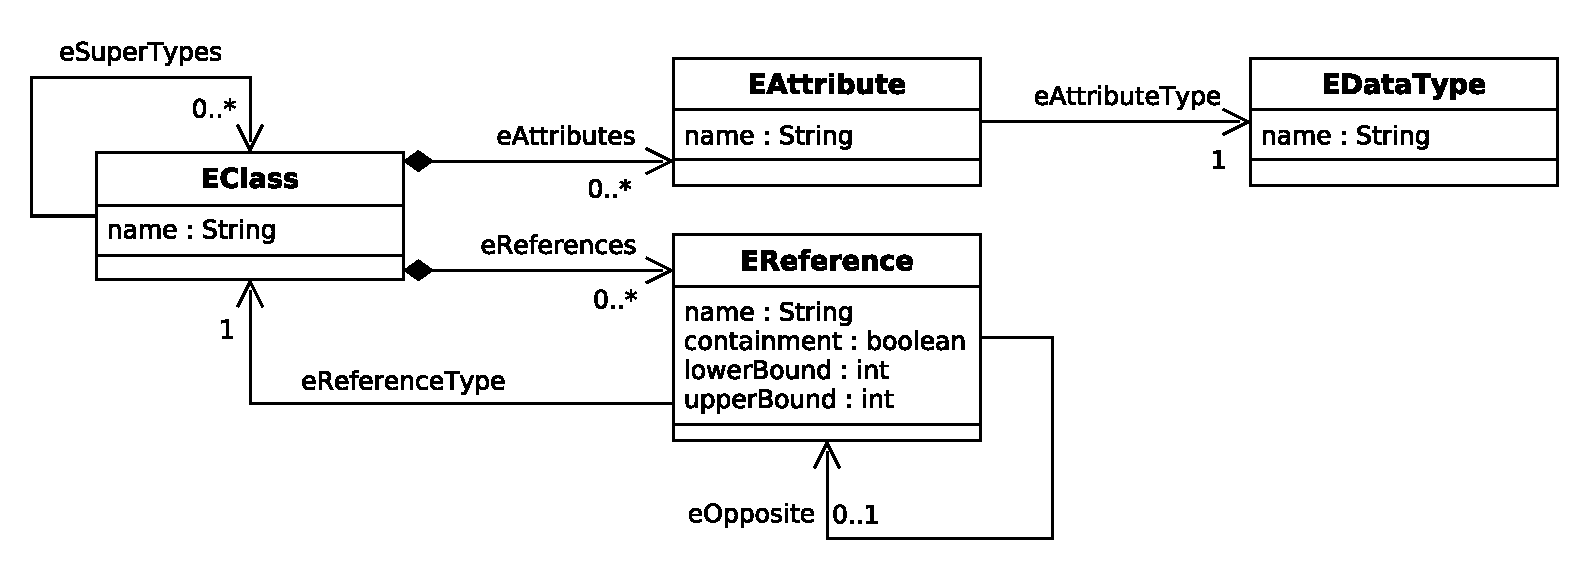
\includegraphics[width=\textwidth]{figures/pdfs/ecore-kernel.pdf}
	\caption{The ECore metamodel}
	\label{fig:ecore}
\end{figure}


\subsubsection{Extension of the ECore}
From an ECore model, the generator of EMF can create a corresponding set of Java implementation classes. Every generated EMF class extends from the framework base class, \eobject, which enables the objects to be integrated and appear in the EMF runtime environment. \eobject provides an efficient reflective API for accessing the properties of the object generically. In addition, change notification is an essential property of every \eobject and an adapter framework can be used to support extension to the objects.

The reflective API~\cite{EMFAPI} \label{sec:emf-reflection}in EMF enables to manipulate all attributes and references attached to the \eobject by using the \texttt{eSet} and \texttt{eGet} functions. This is conceptually equivalent to \texttt{java.lang.reflect.Method.invoke()} Java method, though it is much more efficient in the aspect of performance.
	
 Notification observers (or listeners) in EMF are called adapters~\cite{EMFAdapter} because in addition to their observer status, they are often used to extend the behavior (that is, support additional interfaces without subclassing) of the object they are attached to. An Adapter, as a simple observer, can be attached to any \eobject by simply adding the adapter to the \texttt{eAdapters} list of the \eobject. This Adapter implements a function called \texttt{notifyChanged}, which is called any time when the \eobject, which contains the Adapter, is manipulated. All information about the manipulation is held by a notification object which is the input parameter of the \texttt{notifyChanged} function. This adapter is responsible for sending the notifications to the \texttt{EMFInstanceAdapter} manager class.



\subsubsection{Example EMF metamodel and model of a program ASG}

As an running example, the an EMF metamodel is shown in \autoref{fig:example-mm}, as exported from \emph{ECoreTools}~\cite{ecoretools}. The main parts of the metamodel are the following:

\begin{itemize}
	\item \texttt{Expression} is the superclass for every expression type,
	
	\newcommand{\javaCode}[1]{\lstinline[language=java,keepspaces=true,basicstyle=\ttfamily]!#1!}
	
	
	\item instances of \texttt{Unary} represent expressions that only accept up to one expression as their operand,
	\item instances of \texttt{InstanceOf} stand for \texttt{instanceof} operators in the code,
	\item instances of \texttt{Identifier} represent valid Java identifiers in the ASG,
	\item \texttt{Named} is a superclass of any valid Java ASG element, that is supplied with a name (except for \texttt{Identifier} to avoid loops via the \texttt{refersTo} relation),
	\item instances of \texttt{Parameter} represent parameters in the program, and
	\item \texttt{Handler} marks an exception handler \texttt{catch} block for a \texttt{try-catch} construction in the ASG.
\end{itemize}

\begin{figure}[!htp]
	\centering
	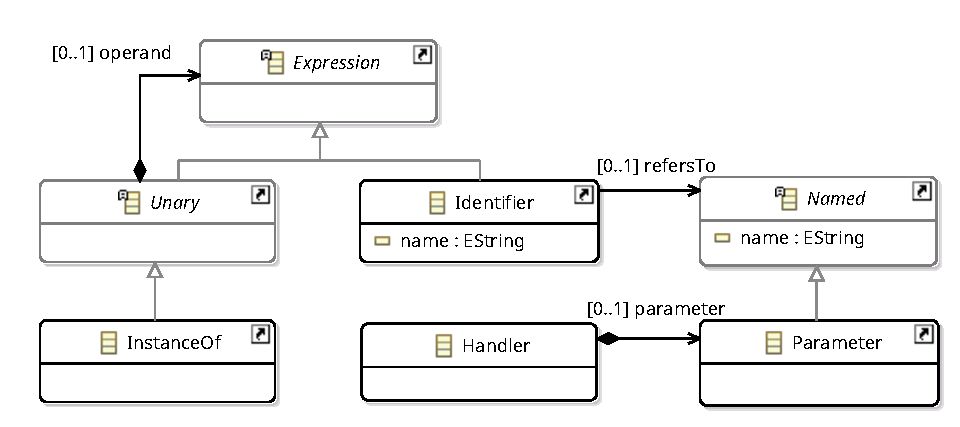
\includegraphics[width=0.9\textwidth]{figures/pdfs/example-metamodel.pdf}
	\caption{EMF metamodel fragment for ASGs}
	\label{fig:example-mm}
\end{figure}

From the explanatory code snippet in \autoref{lst:javaexample}, using the same tool that was used to generate the ASGs of the programs included in~\cite{DBLP:journals/infsof/UjhelyiSHCVVF15}, we obtained the EMF model.
%presented in \autoref{fig:example-instancemodel}, opened in the generated EMF model editor in Eclipse. 
We include a hand drawn version of the instance model in \autoref{fig:example-instancemodel-handdrawn}. It uses simplified object names and applies some trivial abbreviations of the type names. 
%Under every the name and type of every object we included the corresponding line numbers from \autoref{lst:javaexample}. 
Each node in \autoref{fig:example-instancemodel-handdrawn} is adorned with its corresponding line number from  \autoref{lst:javaexample}.
We also used four different colors for the \texttt{Expression}, \texttt{Named}, \texttt{Statement} and \texttt{Handler} types. The subtypes of these types are marked with the same color as the corresponding supertype. Some element types are not shown above in the metamodel fragment, for they would only complicate the structure, and would not help the comprehension of the example. However, we include a more detailed, but still incomplete metamodel in \autoref{fig:example-extended-mm} in the Appendix.

%\begin{figure}[!htp]
%	\centering
%	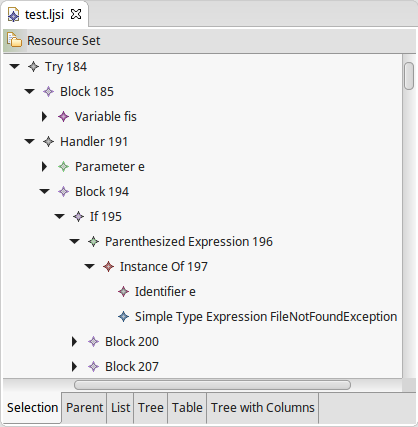
\includegraphics[scale=0.5]{figures/instancemodel-emfeditor}
%	\caption{The EMF instance model opened in the generated editor}
%	\label{fig:example-instancemodel}
%\end{figure}


\begin{figure}[!htp]
	\centering
	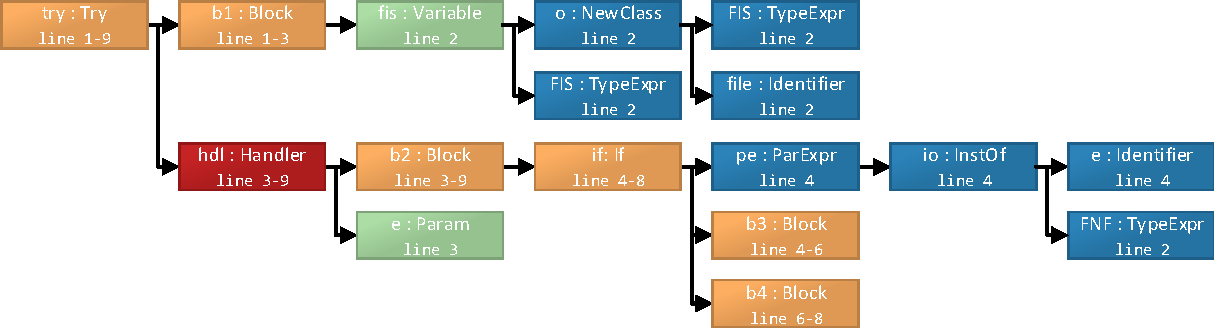
\includegraphics[width=\textwidth]{figures/pdfs/instance_model.pdf}
	\caption{The ASG representation of the example code snippet}
	\label{fig:example-instancemodel-handdrawn}
\end{figure}


%----------------------------------------------------------------------------
\section{Implementing model queries using graph patterns}
%----------------------------------------------------------------------------
\label{sec:graphpatterns}


As described in~\cite{DBLP:journals/scp/UjhelyiBHHIRSV15}, graph patterns are graph-like structures that encapsulate a set of constraints regarding the nodes, the attributes of the nodes, and edges. Model queries can be carried out by matching a graph pattern against instance model graphs. During the matching process the objective is to find suitable model elements that satisfy all constraints of the graph pattern. According to~\cite{DBLP:conf/icmt/BergmannURV11}, \eiq is a framework with a \emph{language for defining declarative queries over EMF models}, and a \emph{runtime engine for executing them efficiently without manual coding}. 

%TODO from what to what and how


\subsection{\eiq pattern language}
\label{sec:patternlanguage}
The framework has its own highly declarative pattern language called IncQuery Pattern Language (IQPL). The language is similar to Datalog, which is a subset of Prolog. As stated in~\cite{DBLP:conf/icmt/BergmannURV11}, the graph pattern based query language of \eiq references \texttt{EClasses} as node types, \texttt{EReferences} and \texttt{EAttributes} as edge types. Pattern variables will be mapped to \texttt{EObjects} of the instance model or attribute values. It is important to add that the language does not specify the order of constraint evaluation.

%\todo{introduce (advanced) language constructs: transitive closure, neg find, count find, check expression, eval}


Based on~\cite{sosym-dslvalidation}, we provide a short summary of the constraints supported by the IQPL:

\begin{itemize}
	\item \textbf{Classifier constraint:} checks if a variable is an instance of an \texttt{EClass}.
	\item \textbf{Path constraint:} requires a specific reference, an attribute, or a path of reference and attribute sequence between two variables.
	\item \textbf{Equality constraint:} specifies that two variables have to be mapped to the same model element.
	\item \textbf{Pattern call constraint:} enables the composition of multiple patterns. The \emph{positive pattern call} refers to another pattern and specifies that the called pattern must be satisfied in the context of the actual parameters. Additionally, a pattern may define a \emph{negative application condition} (\texttt{neg} keyword), which means that the target pattern is disallowed to have a valid match along the actual parameters. Using the \texttt{count} keyword, \eiq can save the \emph{number of matches} to a variable. 
	\item \textbf{Binary transitive closure}: it is possible to describe the \emph{transitive closure} of a two-parameter pattern by the \texttt{+} symbol.
	\item \textbf{Check constraint:} evaluates a specific attribute expression on the variables of the pattern and accept matches only if the result of attribute condition is true.
	\item \textbf{Eval constraint:} evaluates an expression defined inside the constraint. The return value of the evaluation will be stored in a variable.
\end{itemize}



In order to demonstrate the basic capabilities and structural constraints of the language, \autoref{lst:catch} shows the example catch finder problem formulated in IQPL. It introduces two patterns, \catchproblem and \handlervar, both with two symbolic parameters. There are type constraints applied to the parameters: the substitutions of \texttt{cBlock} need to be of type \texttt{Handler}, while \texttt{insOf} is expected to be an \texttt{InstanceOf}. 

% This prevents the listing to be split between pages
\begin{figure}[!htbp]
	\listingiqpl{catch}{Patterns to detect missing catch clauses} 
\end{figure}

The \catchproblem pattern specifies its match set as a set that holds tuples of type $ \langle \texttt{Handler, InstanceOf} \rangle $ in line 1 using classifier constraints for parameters.  In line 2 the pattern declares that the \texttt{varRef} variable should be subtituted with an instance of \texttt{Identifier}, which is also expressed using a classifier constraint. Line 3 prescribes by a path constraint that the \eobject substituted to \texttt{insOf} should have \texttt{varRef} as its \texttt{operand}. In addition, the pattern also uses a pattern call constraint to reference the \handlervar pattern, and the call will use the substitutions of \texttt{cBlock}, and \texttt{varRef} variables.

The latter pattern will have tuples of $ \langle \texttt{Handler, Identifier} \rangle $ in its match set, according to line 7. Line 8 states that the variable \texttt{cBlock} shall have \texttt{param} as its \texttt{parameter}. In line 9 it is specified that the \eobject substituted into \texttt{param} should be navigable from \texttt{variable} via an instance of the \texttt{refersTo} \texttt{EReference}.




\subsection{Incremental pattern matching}

The \eiq framework initially was designed to provide pattern matching capability for its users, based on an incremental pattern matching algorithm (Rete~\cite{bergmann:thesis-queries}). This approach relies on the idea that along with the computation of the initial match set of each pattern, a data structure is built in the memory. This data structure is then maintained in a way that every change in the underlying model is propagated efficiently, so that the set of matches is updated. In case of EMF models this update mechanism implemented using the efficient EMF notification observers of the framework.

%A generic Rete network structure is depicted in \autoref{fig:rete}. This is essentially a dataflow network, where the input data is located in \emph{input nodes}. Each input node contains 
%
%\begin{figure}[!htp]
%	\centering
%	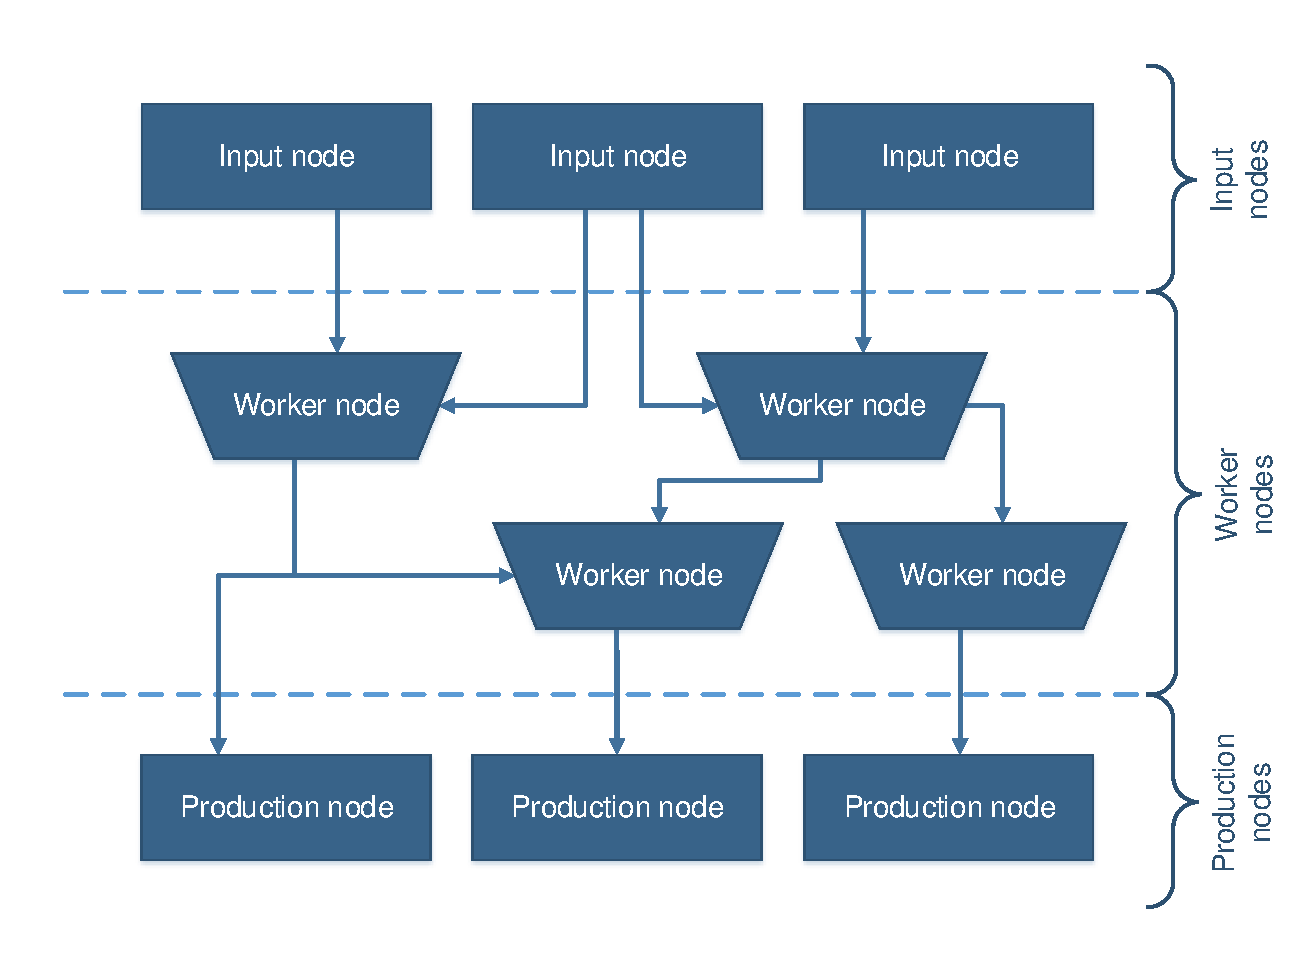
\includegraphics[width=\textwidth]{figures/pdfs/rete.pdf}
%	\caption{Schema for Rete network}
%	\label{fig:rete}
%\end{figure}

To demonstrate this in operation using our example, \autoref{fig:example-rete} depicts a possible  Rete network for the \catchproblem pattern. The Rete network is essentially a dataflow network, where every node contains tuples of arbitrary length. At the top of the diagram rectangles symbolize \emph{input nodes}, which provide input for the network. The second node in the top-left corner is, in addition, a \emph{production node} that means it already holds the match set of the \handlervar pattern. 

\begin{figure}[!htp]
	\centering
	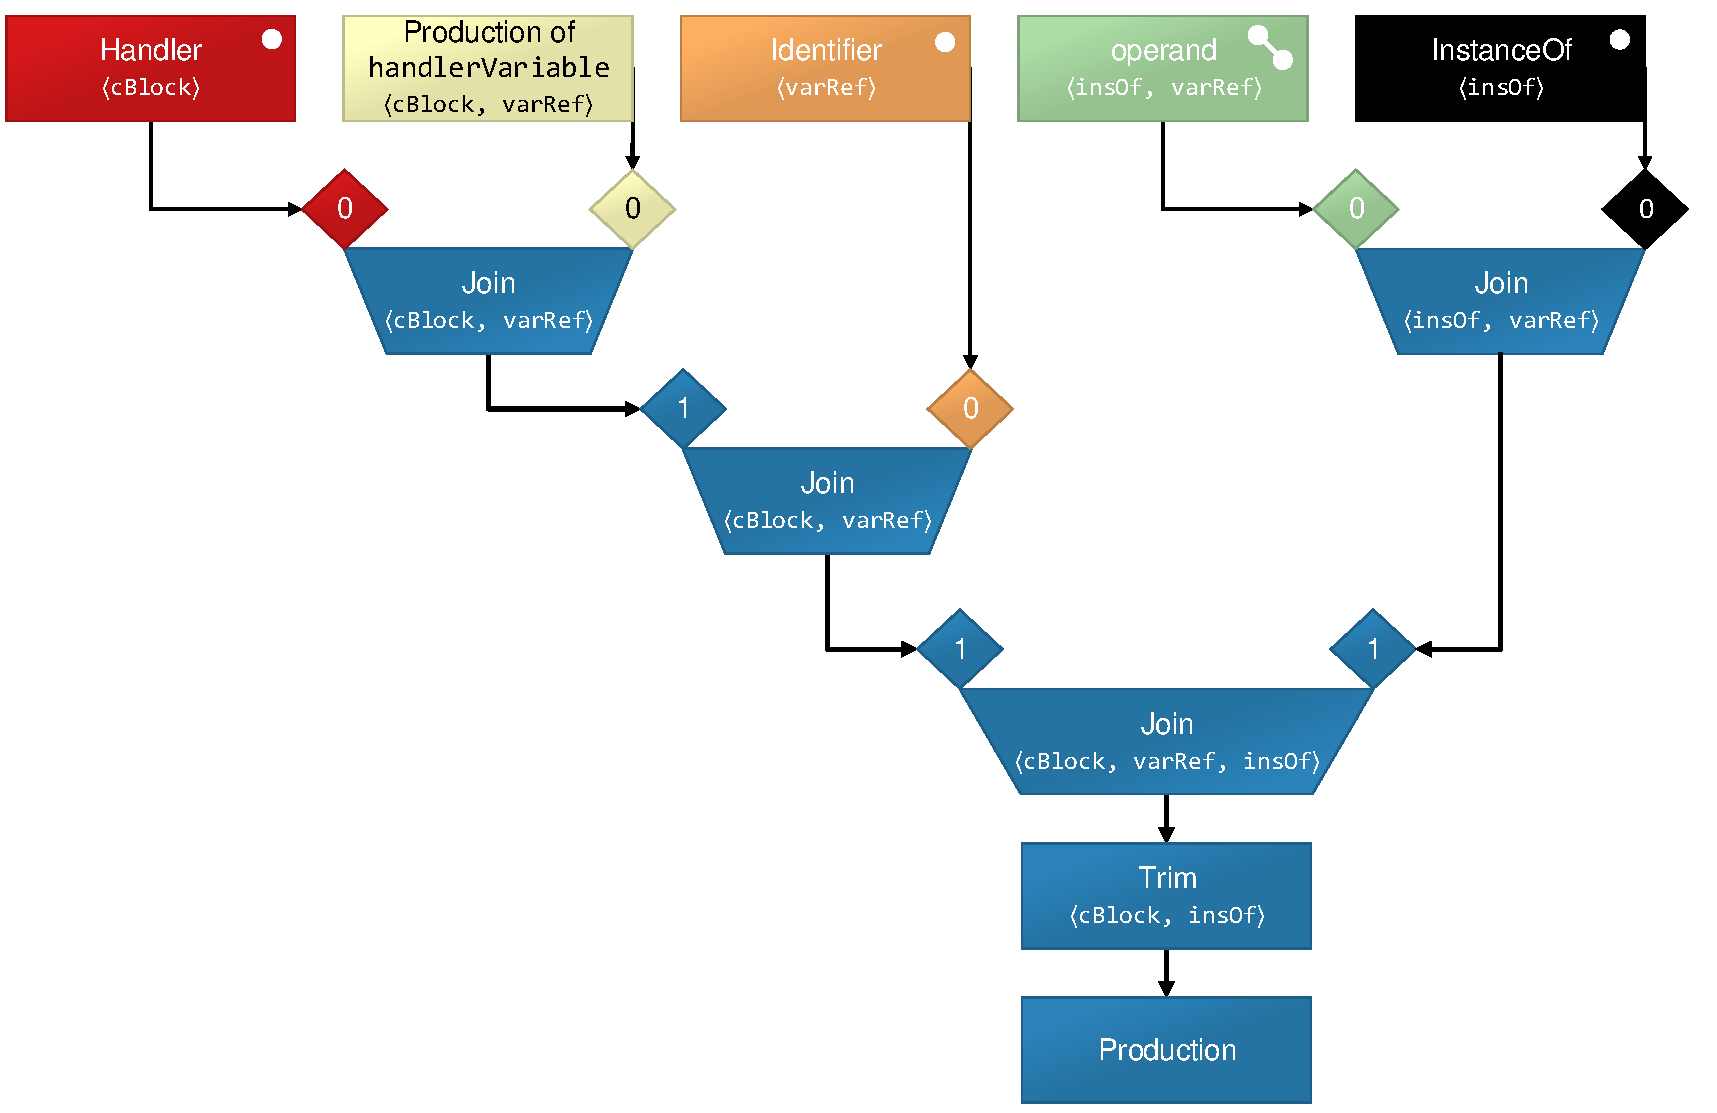
\includegraphics[width=\textwidth]{figures/pdfs/rete-catchProblemFinder-layout.pdf}
	\caption{Rete network for the \catchproblem pattern}
	\label{fig:example-rete}
\end{figure}


Nodes with \emph{Join} annotation are a type of \emph{worker nodes}. They carry out join operation on the input. The diamonds over the worker nodes indicate the operand indices from the previous node. The \emph{Trim} node omits some values from the preceding worker node. In the example, $\langle \texttt{cBlock, varRef, insOf} \rangle $ is trimmed to $\langle \texttt{cBlock, insOf} \rangle $. Finally, \emph{Production} will hold the match set for a pattern.


The main advantage of this solution is the ability to retrieve the match results in constant time after the first evaluation, if the model is unchanged. In case the model changes, the match result update time is proportional to the size of the change, and not the size of the complete model.

In the example, when a new object of type \texttt{Identifier} appears, the change is propagated in the Rete net on a directed path down to the production node. This way matches after small changes in the model are instantly updated.

However, a main drawback of this approach is the memory footprint of the internal data structure. Its size depends on the size of the model and the complexity of the pattern. In certain application scenarios, in which the models themselves are extremely large, this footprint means a bottleneck concerning the usability of the algorithm.


%This summary of the Rete incremental pattern matcher algorithm is based on~\cite{szarnyasg/msc}. The initial version of the algorithm was described in~\cite{DBLP:conf/isca/GuptaFNW86}, and was created for rule-based expert systems. It was adapted and optimized for the Eclipse Modeling Framework by Gábor Bergmann~\cite{bergmanng/msc}. 

%The basis of its operation is an asynchronous network of communicating nodes, which is fundamentally a dataflow network. A generic version of such a structure is depicted in \autoref{fig:rete}. When the algorithm starts, it builds up this network and computes the match set of every pattern. Then, by using notifications from the 

%\begin{figure}[!htp]
%	\centering
%	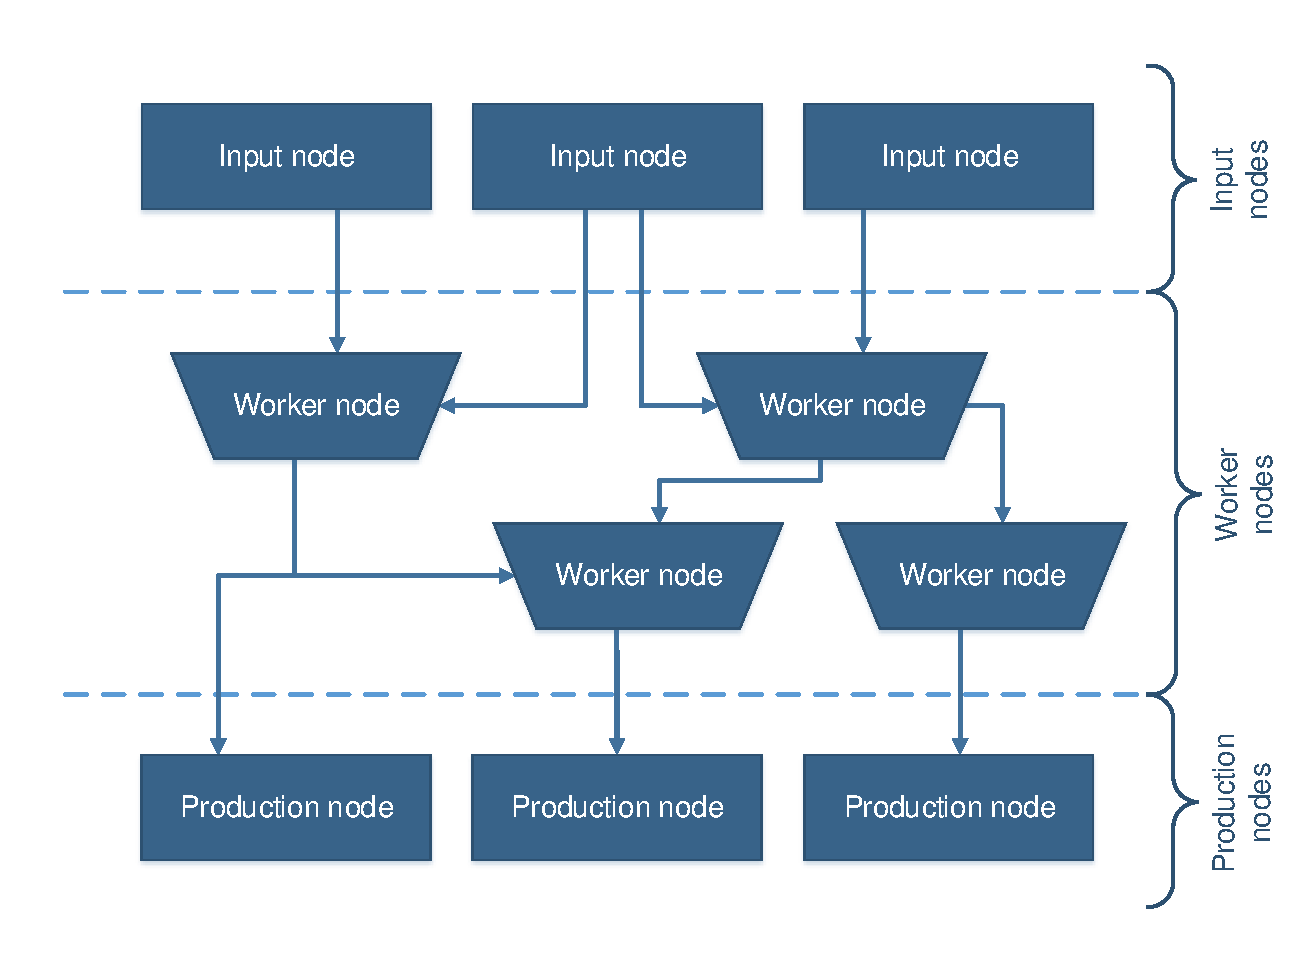
\includegraphics[width=\textwidth]{figures/pdfs/rete.pdf}
%	\caption{The generic stucture of a Rete network}
%	\label{fig:rete}
%\end{figure}
%
%\begin{figure}[!htp]
%	\centering
%	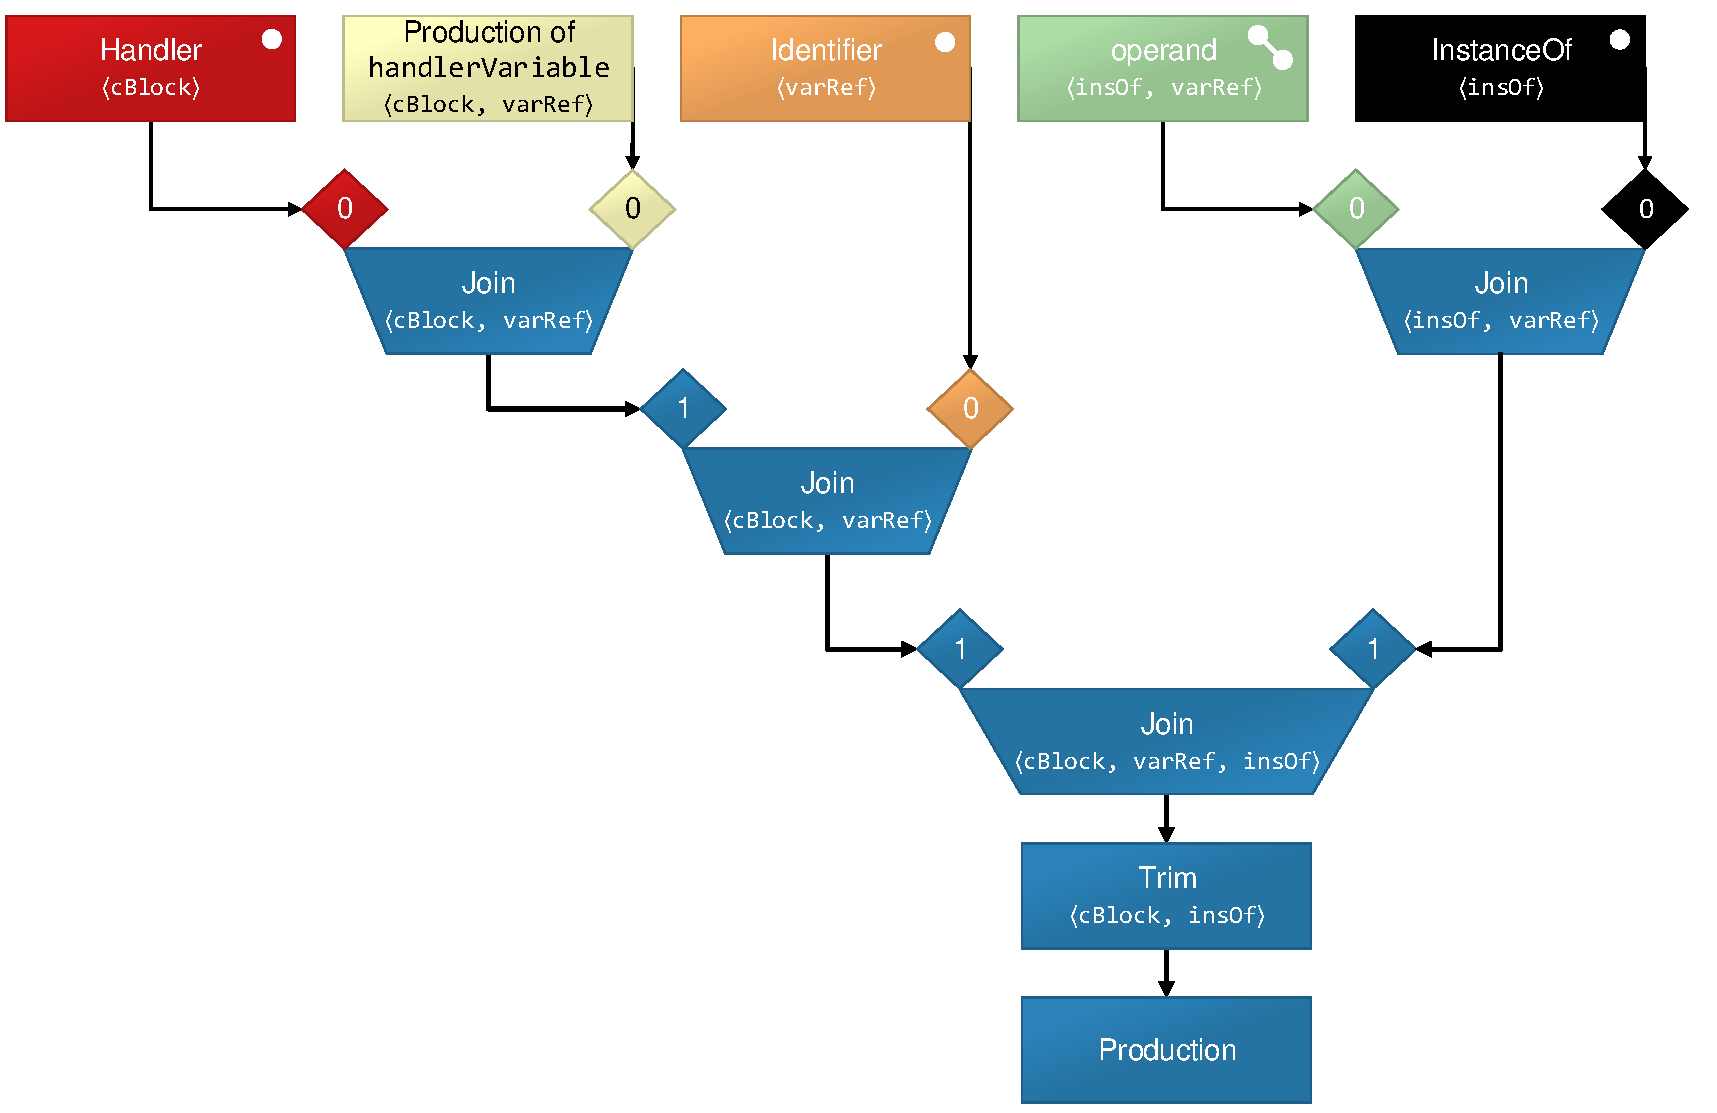
\includegraphics[width=\textwidth]{figures/pdfs/rete-catchProblemFinder-layout.pdf}
%	\caption{The rete network for the catch problem finder query}
%	\label{fig:example-rete}
%\end{figure}

%----------------------------------------------------------------------------
\chapter{Overview of local search-based pattern matching}
%----------------------------------------------------------------------------
\label{chap:overview}


Probably the biggest drawback of the \eiq framework is the memory consumption of its incremental algorithm. In order to overcome this limitation, we adapted a model sensitive local search-based pattern matching algorithm described in \cite{DBLP:journals/sosym/VarroDWS15}. This algorithm has a much smaller memory footprint, as well as the initial pattern matching execution takes also less time compared to the Rete incremental approaches.


\section{Related work}
\label{sec:relatedwork}

There are several modeling tools that implement pattern matching in addition to \eiq, such as ATL, Eclipse OCL, FUJABA, FunnyQT, and GrGen.NET. 

\emph{ATL}~\cite{DBLP:conf/uml/JouaultK05} defines a hybrid, textual language for defining graph transformations. It is called hybrid, for it has declarative language elements, but in order to ease formulation of complex rules, imperative instructions can also be used. ATL uses local search-based pattern matching, but applies different heuristics to determine the order of search operations. As it was described in~\cite{DBLP:conf/models/TisiPC13}, a parallel algorithm provides the matchings. %Also, the ATL has support for execution over various modeling domains, like...

\emph{Eclipse OCL}~\cite{eclipse:ocl} supports the declarative definition, and evaluation of OCL~\cite{OCL:Spec} constraints over EMF models. In this case, despite the declarative description of the pattern, the OCL constraint encodes the execution order of search steps to find elements that conform all constraints of the description. Also, Eclipse OCL has incremental evaluation support~\cite{DBLP:journals/jss/CabotT09}.

%\emph{FUJABA}~\cite{DBLP:conf/icse/NickelNZ00} provides a graphical language for specifying model transformation rules, and relies on local search-based pattern matching. It uses a breadth-first traversal of \emph{search graphs} with edge weights based on the multiplicity of references, as opposed to our adapted model-sensivive, dynamic programming based search plan calculation.

\emph{FUJABA}~\cite{DBLP:conf/icse/NickelNZ00} provides a graphical language for specifying model transformation rules, and relies on local search-based pattern matching. It uses \emph{story diagrams} for the execution~\cite{DBLP:journals/eceasst/GieseHS09}, and applies a dynamic strategy concerning the traversal of the instance model. This means for every object, the following step is made in the direction of the reference with the lowest multiplicity. The execution times presented in~\cite{DBLP:journals/eceasst/GieseHS09} are very promising regarding this approach. We can say that \emph{SDMLib} is the successor of FUJABA, which won the best performance award on the Transformation Tool Contest 2014~\cite{DBLP:conf/staf/EickhoffGLZ14} by generating Java code for search execution.

\emph{FunnyQT} is a Clojure library supplying a comprehensive set
of model querying and transformation services to the user~\cite{DBLP:conf/gg/Horn15}. According to~\cite{DBLP:conf/icmt/Horn13}, it supports pattern matching using an internal DSL implemented with Clojure’s metaprogramming facilities. The constraint evaluation order is defined by the user. 

\emph{GrGen.NET}~\cite{DBLP:conf/agtive/BatzKG07} also implements pattern matching based on local search philosophy. It calculates search plans based on a cost model, that estimates a \emph{backtracking} and an \emph{execution time} for an operation. The used search plan has the lowest total cost of operations possible. 

The algorithm we introduce in this work uses a search plan calculation algorithm that differs from the ones mentioned above. Also, the \eiq framework is unique in a way that the declaratively defined patterns can be executed using any of the local search or the incremental algorithm, without specifying the concrete steps of the execution.


\section{Algorithm adaptation}
\label{sec:algorithm-adaptation}
%TODO adaptation description?

In order to efficiently integrate the local search-based algorithm, we were required to adapt many existing components of the \eiq framework, more specifically parts of the \emph{pattern matcher engine}. The architecture overview of the engine is depicted in \autoref{fig:overview_core}:

\begin{enumerate}
	\item \emph{\baseindex} collects the instances of \texttt{EClasses}, \texttt{EReferences} and \texttt{EDataTypes} contained in a model,
	\item the \emph{Pattern definition} holds the query that is to be evaluated over the instance model, 
	\item the \emph{Pattern matcher} uses the pattern matcher algorithm to generate the result based on the \eiq Base Index and the Pattern definition, and
	\item the \emph{Match set} contains the result tuples.
\end{enumerate} 

\begin{figure}[!htp]
	\centering
	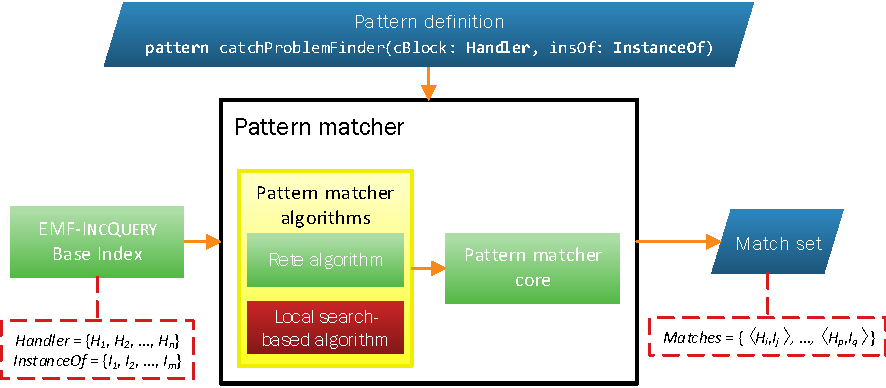
\includegraphics[width=\textwidth]{figures/pdfs/overview_core.pdf}
	\caption{The pattern matcher engine of \eiq}
	\label{fig:overview_core}
\end{figure}

In the introductory example, the base index would provide sets filled with the instances of the elements found in the metamodel, such as \texttt{Handler} and \texttt{InstanceOf}, as indicated in the lower left corner of \autoref{fig:overview_core}. The \catchproblem pattern definition states that the expected matches are supposed to be tuples with type $\langle \mathtt{Handler, InstanceOf}\rangle$, as illustrated below the match set in the diagram.

Our contribution to the engine (emphasized with solid red background) is the \emph{local search-based algorithm}, at least in the extent of this thesis. Prior to the implementation, we solved several adaptation issues.  A typical task was to decide how to extend already existing interfaces in order to obtain all the information needed for executing the algorithm. One of the main design guidelines was generalization of the existing solution, so that several pattern matching algorithms may coexist in the \eiq framework.

In as a result of our work, we proposed a common interface for pattern matching algorithms. In addition, using the chosen solution, users can select the appropriate algorithm runtime, according to their needs. We also prepared the pattern matcher runtime for parallel search execution, for the computation of matches can be done by multiple threads simultaneously. The details about search execution is in \autoref{sec:search-execution}.

While the \emph{Graph pattern matcher engine} provides the basic functions of \eiq, there are many accompanying tools to ease the use of the provided features. To introduce the layered architecture of the toolkit based on \cite{DBLP:journals/scp/UjhelyiBHHIRSV15}, a diagram of its structure is shown in \autoref{fig:overview}. 

\begin{figure}[!htp]
	\centering
	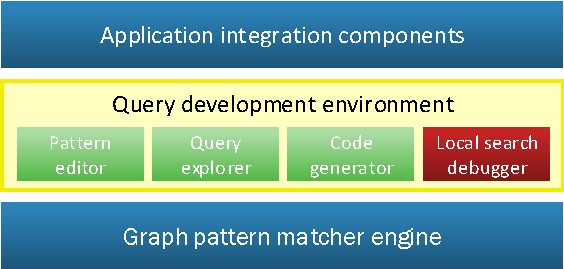
\includegraphics[width=0.7\textwidth]{figures/pdfs/overview}
	\caption{The architecture of \eiq}
	\label{fig:overview}
\end{figure}

The \emph{Query development environment} (QDE) provides tooling related to defining and debugging queries. One of the major components is the (i) \emph{Pattern editor}. This is an Xtext-based \cite{Xtext} editor for IQPL with syntax highlighting, auto-completion support and pattern well-formedness validation. The purpose of the (ii) \emph{Query explorer} is to evaluate complex queries on selected EMF models, and to visualize the match set of each pattern. Another very important part of the QDE is the (iii) \emph{Code generator}. It is tightly connected to the editor, as well as registered into the Eclipse builder framework. Thanks to this strong coupling with the IDE, code generation is executed after pattern definitions are modified, and saved. The output of the generation process is a pattern-specific Java code, that helps the integration of \eiq to Java applications by creating type-safe API for matchers. 

To further extend the capabilities of the QDE, we developed a (iv) \emph{Local search debugger} (highlighted with solid red background in the overview). It is designed to help the pattern developers understand and debug the local search-based pattern matching process by providing a visual representation of the calculated search plan, and to support step-by-step execution capability. \autoref{sec:lsdebugger} introduces the new debugger component and its capabilities in detail.


\eiq provides several application integration components as well, as indicated in the top part of \autoref{fig:overview}. They are not discussed in this work in detail, but they provide an API for accessing the features of the \eiq framework from Java programs.


\section{Pattern matching workflow}
\label{sec:pattern-matching-workflow}

We separate the local search-based pattern matching tasks into two categories. The first category is \emph{design time} tasks, and the second is \emph{execution time} tasks. Our pattern matching workflow is depicted in \autoref{fig:workflow}.

\begin{figure}[!htp]
	\centering
	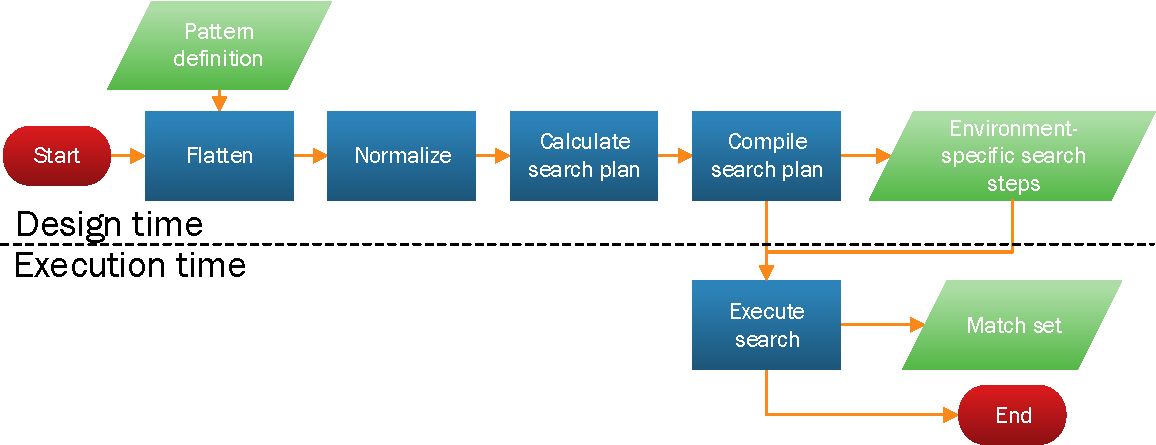
\includegraphics[width=\textwidth]{figures/pdfs/query_execution_workflow.pdf}
	\caption{The local search-based pattern matching workflow}
	\label{fig:workflow}
\end{figure}

The majority of the steps of the workflow are considered to be \emph{design time} tasks. The first task is to \emph{flatten} the input \emph{pattern description}. The pattern description may refer to other patterns, and flattening means the resolution of these references. As a result, a \emph{flat pattern} is created that unifies all constraints and variables, both from the referrer and the referee patterns. This allows to optimize on a global scale, rather than locally for patterns. It is important to add that semantics of the pattern is preserved throughout the process. Details about the implemented flattener algorithm is discussed in \autoref{sec:flattening}.

In the next step the flattened pattern is \emph{normalized}. This means an analysis in order to remove redundant, thus unnecessary constraints. For instance, type checking multiple times for the same variable, and with the same type is omitted. This step also unifies variables among equalities.

From the normalized pattern the \emph{local search planner} calculates a \emph{search plan} in the third step of the above workflow. In this case, this means an ordering of the constraints contained in the pattern. At this point all constraints and variables are directly contained in a normalized, flattened pattern that provides a global search space for the search plan calculation. As it was already mentioned in \autoref{sec:patternlanguage}, the declarative definition of patterns using IQPL does not hold information about the order of constraint enforcement and computation of the matches of a pattern. This requires the local search planner component to create the search operation sequence that finds substitutions for variables. This list of search operation is derived from an ordered list of constraints, which is done in \emph{compile search plan} step. The outcome of design time tasks is a list of \emph{environment-specific search steps}. In case of EMF, these environment specific search operations heavily rely on the efficient EMF reflective API, which is introduced in \autoref{sec:emf-reflection}, to obtain possible substitutions for the variables.

During \emph{execution time}, this list of search steps determines the order of variable substitutions. In the \emph{execute search} phase, the executor looks for substitutions that satisfy all constraints of the pattern. In the current application, it means that at some point, each variable is assigned a model element to check if it satisfies the description of the pattern. The details of search plan execution is detailed later in \autoref{sec:search-execution}.

To demonstrate the effects of the tasks depicted in \autoref{fig:workflow}, the flattened version of the \catchproblem pattern is presented in \autoref{lst:catch_flat} under the name \mbox{\texttt{catchProblemFinder\_flattened}}. 

% This prevents the listing to be split between pages
\begin{figure}[!htbp]
\listingiqpl{catch_flat}{Flattened pattern} 
\end{figure}

The body has all constraints from both \catchproblem and \handlervar, as well as additional equalities that declare the variables used to serve as parameters for the pattern call constraint, and the corresponding variables from the flattened pattern are equal. New variables coming from the flattening process are prefixed with "\handlervar\_".


A normalized version of the \mbox{\texttt{catchProblemFinder\_flattened}} pattern is \mbox{\texttt{catchProblemFinder\_flattened\_normalized}} (contained in \autoref{lst:catch_flat_normalized}). To achieve better readability of the created pattern description, we unified the variables with longer names into variables with shorter names along equalities, and also simplified the name of \texttt{handlervar\_param} to \texttt{param}.  

% This prevents the listing to be split between pages
\begin{figure}[!htbp]
	\listingiqpl{catch_flat_normalized}{Normalized pattern} 
\end{figure}

From the flattened and normalized pattern description, the search plan depicted in \autoref{tab:flat-norm} can be obtained. The details of the search plan calculation is included in \autoref{sec:localsearch}

\begin{table}[h]
	\centering
	\begin{tabular}{c|l}
		\hline
		& Constraint \\ \hline
		1: & \texttt{varRef} is of type \texttt{Identifier} \\
		2: & \texttt{varRef} is in \texttt{operand} relation with \texttt{insOf} \\
		3: & \texttt{insOf} is of type \texttt{InstanceOf} \\
		4: & \texttt{varRef} is in \texttt{param} relation with \texttt{refersTo} \\
		5: & \texttt{param} is referenced by \texttt{cBlock} in \texttt{parameter} \\
		6: & \texttt{cBlock} is of type \texttt{Handler} \\
		
	\end{tabular}
	\caption{Search plan for the flattened pattern}
	\label{tab:flat-norm}
\end{table}

If we compile the search plan for our introductory EMF-based example as the final step of the design time tasks, the list of environment specific search operations will be the following:
\begin{enumerate}
	\item Collect all instances that are of type \texttt{Identifier}. Then, one-by-one substitute the values to variable \texttt{varRef} and advance to the next search operation.
	\item For the current value of \texttt{varRef}, enumerate all values which can navigate to it on an \texttt{operand} reference. Substitute each enumerated element to \texttt{insOf}, then go on to the next operation.
	\item Check if the type of the substituted element for variable \texttt{insOf} is \texttt{InstanceOf}.
	\item Get all elements reachable from \texttt{varRef} by navigating on the \texttt{param}  relation. Substitute each element reached this way in place of variable \texttt{refersTo}, then advance to the next operation.
	\item Collect all elements that have the value of \texttt{param} in their \texttt{parameter} relation, then substitute each to \texttt{cBlock}.
	\item Check if \texttt{cBlock} has a substituted element of type \texttt{Handler}.
\end{enumerate}

This step is then followed by the \emph{execution task} on the given instance model. During the execution in this current minimal example, there are only a few elements in every steps that should be considered. There is only one match in this case, a tuple that is $ \langle \mathtt{hdl}, \mathtt{io} \rangle$ (using the notation of the hand drawn instance model in \autoref{fig:example-instancemodel-handdrawn}).

% !TEX encoding = UTF-8 Unicode
%----------------------------------------------------------------------------
\chapter{Integration to \eiq}
%----------------------------------------------------------------------------
\label{chap:integration}

%TODO kb. 16-27 oldal

In this chapter the design and integration challenges are discussed in details. The implemented local search-based algorithm is from the paper \cite{DBLP:journals/sosym/VarroDWS15}. The main advantage of this algorithm is its adaptive model sensitive approach for calculating search plans. It means that the properties of the instance model, on which the search plan calculation is executed, are considered. In this work we only introduce the main differences and key ideas that were required for a successful implementation and integration.

%----------------------------------------------------------------------------
\section{Details of the adapted algorithm}
%----------------------------------------------------------------------------
\label{sec:details}


%TODO kb. 5-10 oldal

The published paper~\cite{DBLP:journals/sosym/VarroDWS15}, which served as the basis of our implementation, is about pattern matching over EMF models. However, it did not include any programming source code, only pseudo code. For this reason, we adapted it to be executable on a JVM, and to also fit into the internal design of \eiq. The current section introduces the concept of search plan, and the outline of the search plan calculation algorithm, along with an illustration of its execution on our running example. For a fully comprehensive description please refer to the article cited above.

%As we mentioned at the beginning of \autoref{chap:integration}, including every detail about the implemented search algorithm is far beyond the scope of this thesis, but the basic idea of search plan calculation is introduced in \autoref{sec:localsearch} for the better comprehensibility of our work.  

\subsection{Search plan}
\label{sec:localsearch}
	 
	 
A search plan, in our case, means an ordered list of constraints of the pattern definition. As it was discussed in \autoref{sec:pattern-matching-workflow}, the list of executable environment specific search steps are obtained by compiling the search plan. This compilation is simply a mapping between constrains and search steps, which only depends on the properties of the target modeling environment. For this reason, in the following we are only concerned about the search plan calculation. In the following we will refer to elements of the search plan as \emph{search operations}, and we will represent them with the corresponding constraint from the query definition.


In order to clarify the purpose of the search plan, we define the concepts of \emph{free variables} and \emph{bound variables}. They can be interpreted as follows: if the search execution of the search plan was halted at a given point, which variables would already be assigned to a model element, and which variables would not have values yet. Variables without associated values are called \emph{free variables} (\texttt{F}), and variables with assigned values are referred as \emph{bound variables} (\texttt{B}). 

The \emph{pattern adornment} denotes the initial binding state of the parameter variables of a pattern at the beginning of the pattern matching, in other words describes witch parameter variables have initial values. The purpose of the search plan is to guide the search execution in a way that by reaching the end of the search plan each variable should already be bound.



The search operations can be categorized according to the binding state of the variables affected by the corresponding constraint. Two basic categories of search operations are \emph{extend}, and \emph{check}. A \emph{check operation} verifies whether a variable substitution is in compliance with a constraint included in the pattern. This means that in case of a check, every variable of the operation is bound by the time of its execution. On the other hand, an \emph{extend operation} has a list of substitution values for a variable, where these values are selected based on the corresponding constraint. During the search, all the elements in this list are to be substituted in order to find all matches in the model.

As a corollary of the definitions of check and extend operations, we can say that the position of the operation in the search plan decides to which category it belongs. However, there are some disallowed extend cases, which require a significant computational capacity during search execution, thus they are to be avoided in a search plan. For instance, negative pattern calls should always be check operations.


%For instance, if base index is not built over a model, we inverse navigation along references without inverse navigability support would require an iteration over every object in the domain of the type of the source element of the reference.



In the example, to find all occurrences in a given ASG of the code smell described by \catchproblem, the initial adornment should be \texttt{FF}, which means both \texttt{cBlock} and \texttt{insOf} parameters are unbound at the start of the pattern matching process. A possible search plan for the \catchproblem pattern is included in \autoref{tab:catchproblemOriginal}.

\begin{table}[h]
	\centering
	\begin{tabular}{c|l|c|c}
		\hline
		& \multicolumn{1}{|c|}{Operation} & Type & Bound variables \\ \hline
		1: & \texttt{Indentifier(varRef)} & extend & $\{ \}$\\
		2: & \texttt{Unary.operand(insOf, varRef)} & extend & $\{ \texttt{varRef} \}$\\
		3: & \texttt{InstanceOf(insOf)} & check & $\{ \texttt{varRef, insOf} \}$\\
		4: & \handlervar$(\texttt{cBlock, varRef})$ & extend & $ \{\texttt{varRef, insOf}\} $ \\
		5: & \texttt{cBlock} is a \texttt{Handler(cBlock)} & check & $ \{\texttt{varRef, insOf, cBlock}\} $ \\
	\end{tabular}
	\caption{Search plan for pattern \catchproblem}
	\label{tab:catchproblemOriginal}
\end{table}

For there are no bound variables initially, the search plan starts with an extend operation. In this case it is an enumeration of instances of type \texttt{Identifier}. In the next step, by an \emph{inverse navigation} from the bound \texttt{varRef} variable, along the \texttt{operand} relation possible elements for \texttt{insOf} are collected. When using the \eiq Base Index over a model, inverse navigation along edges are possible, even if the reference has no inverse in the metamodel. The third step is a check operation, which makes sure whether the value of \texttt{insOf} is of type \texttt{InstanceOf}. The fourth operation is an extend, for it binds the \texttt{cBlock} variable by calling the pattern \handlervar with an adornment \texttt{FB}. As the result of the pattern call, each possible \texttt{Handler} block is collected for the value of \texttt{varRef}. In the final step of the search plan, the substituted value for \texttt{cBlock} is verified to be of type \texttt{Handler}. Note, that after the last search operation all variables are bound.

The search plan for the referred \handlervar pattern with initial pattern adornment \texttt{FB} is shown in \autoref{tab:handlervarOriginal}. 
However, we do not introduce the execution steps, because it is very similar to the steps of the search plan introduced for the \catchproblem pattern, except its initial pattern adornment is \texttt{BF}, which means that \texttt{cBlock} already has an assigned value.

\begin{table}[h]
	\centering
	\begin{tabular}{c|l|c|c}
		\hline
		& \multicolumn{1}{|c|}{Operation} & Type & Bound variables \\ \hline
		1: & \texttt{Handler(cBlock)} & check & $\{ \texttt{cBlock} \}$\\
		2: & \texttt{Handler.parameter(cBlock, param)} & extend & $\{ \texttt{cBlock} \}$\\
		3: & \texttt{Identifier.refersTo(variable, param)} & extend & $\{ \texttt{cBlock, param} \}$\\
		4: & \texttt{Identifier(variable)}  & check & $\{ \texttt{cBlock, param, variable} \}$\\
	\end{tabular}
	\caption{Search plan for pattern \handlervar}
	\label{tab:handlervarOriginal}
\end{table}


To demonstrate the importance of flattening and normalization, we include a possible search plan for the pattern from \autoref{lst:catch_flat_normalized} in \autoref{tab:catch_flat_normalized}. As we previously discussed in \autoref{sec:pattern-matching-workflow}, the flattened and normalized patterns have the same semantics as the original. However, the search plan for the normalized pattern is \emph{simpler} than the two original search plans together, where by simple we mean it has less steps of the same operation type than the search plans calculated for the original descriptions.

%TODO introduce alternative search plans?

\begin{table}[h]
	\centering
	\begin{tabular}{c|l|c|c}
		\hline
		& \multicolumn{1}{|c|}{Operation} & Type & Bound variables \\ \hline
		1: & \texttt{Identifier(varRef)} & extend & $\{ \}$ \\
		2: & \texttt{Unary.operand(insOf, varRef)} & extend & $\{ \texttt{varRef} \}$\\
		3: & \texttt{InstanceOf(insOf)} & check & $\{ \texttt{insOf, varRef} \}$\\
		4: & \texttt{Identifier.refersTo(varRef, param)} & extend & $\{ \texttt{insOf, varRef} \}$\\
		5: & \texttt{Handler.parameter(cBlock, param)}  & extend & $\{ \texttt{insOf, varRef, param} \}$\\
		6: & \texttt{Handler(cBlock)}  & check & $ \stackedlines{ \texttt{\{insOf, varRef,}}{\texttt{param, cBlock}\}} $ \\
		
	\end{tabular}
	\caption{Search plan for the flattened and normalized pattern}
	\label{tab:catch_flat_normalized}
\end{table}




\subsection{Search plan calculation}

To find the ordering of the constraints that yields an efficient search plan is a non-trivial task. To estimate the time needed to execute the matching, we can assign \emph{costs} to search operations, and from the individual costs of the operations we can derive the cost for the complete search plan. \emph{Cheap} search plans are desired, for it means that the search can finish faster according to our cost estimation.

In addition to \autoref{tab:catch_flat_normalized}, the search plan listed in \autoref{tab:catch_flat_normalized_from_debugger} can also be used to find matches for the \catchproblem pattern, they only differ in the order of operations. It is model-dependent, which provides faster execution.

\begin{table}[h]
	\centering
	\begin{tabular}{c|l|c|c}
		\hline
		& \multicolumn{1}{|c|}{Operation} & Type & Bound variables \\ \hline
		1: & \texttt{Handler(cBlock)} & extend & $\{ \}$\\
		2: & \texttt{Handler.parameter(cBlock,param)} & extend & $\{ \texttt{cBlock} \}$\\
		3: & \texttt{Identifier.refersTo(varRef, param)} & extend & $\{ \texttt{cBlock, param} \}$\\
		4: & \texttt{Identifier(varRef)} & check & $\{ \texttt{cBlock, param, varRef} \}$\\
		5: & \texttt{Unary.operand(insOf, varRef)}  & extend & $\{ \texttt{cBlock, param, varRef} \}$\\
		6: & \texttt{InstanceOf(insOf)}  & check & $ \stackedlines{ \texttt{\{insOf, varRef,}}{\texttt{param, cBlock}\}} $ \\
		
	\end{tabular}
	\caption{An alternative search plan for \catchproblem}
	\label{tab:catch_flat_normalized_from_debugger}
\end{table}

\subsubsection{Calculating the cost of a search plan}

The search plan calculation algorithm described in~\cite{DBLP:journals/sosym/VarroDWS15} proposes a method to calculate \emph{operation weight} to encode the estimated costs of the operations and search plans. Our current implementation of the algorithm applies the proposed solution with minor modifications.

The main idea is to take every constraint form the pattern, and generate search operations with all possible and allowed variable binding combinations. This means, for every constraint it generates $2^a$ search operations, where $a$ is the number of variables affected by the constraint. This could results in several search operation objects, however, typically constraints have 1 or 2 variables, and for pattern call constraint, we only allow \texttt{BB\ldots B} adornments. We can say that in practical applications, the result search operation set will not reach extreme sizes typically. In the final search plan \emph{each constraint will be represented by exactly one search operation}, and the unused ones will be discarded.
 
Along with the creation of search operations, an estimated number of potential substitutions values is calculated, which the executor has to check each time, when it is executed. This number is then used as its \emph{weight} or \emph{cost}. This means that check operations have a weight of 1, for they only verify whether the current substitutions satisfy a constraint. 

For extend operations, we distinguish several cases. If the operation affects only one variable, which is in case of \eiq means a type constraint, then the cost of the operation is the cardinality of the type required by the constraint. In case of operations enforcing an IQPL path expression, which define that two model elements are connected by an \texttt{EReference} instance, there can be three cases according to the binding state of the of the affected variables:

\begin{itemize}
	\item \texttt{FF}: this operation adornment is disallowed.
	\item \texttt{BF}: in this case the cost is estimated with the \emph{average branching factor}, given by the formula $\textit{weight} = \dfrac{\textit{cardinality of source class}}{\textit{number of links}}$.
	\item \texttt{FB}: similarly to the previous case, the average branching factor is calculated by \\$\textit{weight} = \dfrac{\textit{cardinality of target class}}{\textit{number of links}}$.
\end{itemize}

Every other type of constraint, that is not flattened or normalized (\texttt{count find}, \texttt{neg find}, and inequality) are not allowed as extend operations, for they would typically require unmanageable search times. Positive pattern calls are at the moment always flattened.
%, which often can even be infinite, \eg for inequality.

The cited article distinguishes other constraint types as well, such as ternary constraints for ordered references, but in \eiq there is no support to directly input such constraints yet.

From the $w_{o_{k}}$ costs for each $o_k$ operation, where $k$ represents the position in the search plan, the total cost $C_n$ of a search plan containing $n$ search operations is calculated with the following recursive formula:

$$ C_n = \sum_{i=1}^{n} \prod_{j=1}^{i} w_j = C_{n-1} + w_{o_{1}} \cdot w_{o_{2}} \cdots \cdot w_{o_{n}}. $$
\label{sec:cost}

\subsubsection{Dynamic programming based search calculation}

With the above definition of search plan cost, a dynamic programming based approach is used to create search plans that are cheap in this sense. The algorithm outline is as follows:

\begin{enumerate}
	\item Initialize a table with dimensions $d \times (f+1)$, where $d$ is an input parameter of the algorithm. We call it \emph{drop threshold}, because it influences which search plans are considered too expensive during the planning process, and thus ignored in later steps. The $f$ symbolizes is the \emph{number of free variables} in the initial adornment of the pattern. Each column symbolizes the number of free variables, and each cell represents a search plan. Column indices go from $f$ to $0$.
	\item Starting from the $f$th column, we begin filling out the table using the rules below:
		\begin{itemize}
			\item Based on a previous search plan, we pick an \emph{applicable} extend operation, which means every variable affected by the operation and marked with \texttt{B} in its adornment is bound by the end of the previous search plan, and every variable marked with \texttt{F} in the operation adornment is free at the end of the selected, preceding search plan. When done, we append it to the search plan. In case we are filling out the $f$th column, and there is no preceding, then create a new one instead.
			\item Append all applicable check operations to the search plan, then calculate a new cost using the recursive formula.
			\item Insert search plans calculated this way in an increasing cost order to the table, and simply drop search plans that do not fit. The number of search plans in a column is determined by the parameter $d$.
		\end{itemize}
	\item Select the plan that is in the intersection of the first row and $0$th column, because has the lowest cost, and yields \texttt{BB\ldots B} variable binding after its final step.
\end{enumerate}


Two steps of the running algorithm on the model depicted in \autoref{fig:example-instancemodel-handdrawn}  is demonstrated in \autoref{fig:plan-calculation-example} by filling up the columns 4, 3 and 2 of the table of search plans. The $d$ parameter is set to $2$.

\begin{figure}[!htp]
	\centering
	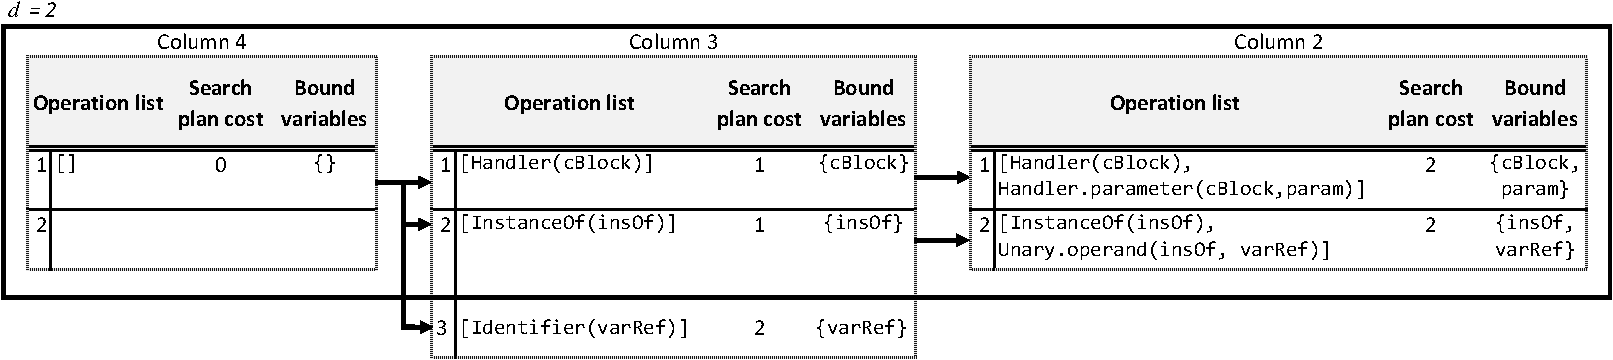
\includegraphics[width=\textwidth]{figures/pdfs/plan-calculation.pdf}
	\caption{Table of search plans}
	\label{fig:plan-calculation-example}
\end{figure}

Initially column 4 contains only one entry, which is a search plan with an empty list of operations, total cost of 0, and an empty set of bound variables. Based on the variable binding, the applicable constraints are \texttt{Handler(cBlock)}, \texttt{Identifier(varRef)}, and \texttt{InstanceOf(insOf)}, all with adornment \texttt{F}. 

In the first step, the cost of the search plans containing only one of them is calculated. Using the recursive cost formula, it gives the cost of the operation plus the cost of the preceding search plan, which is in this case 0. Based on the instance model the costs are 1 for \texttt{Handler(cBlock)}, 2 for  \texttt{Identifier(varRef)}, and 1 for \texttt{InstanceOf(insOf)}. The search plans are then inserted into column 3 in increasing cost order. We chose $d = 2$, so the third search plan is discarded, which means it is not stored in the table, thus not used as the basis of latter search plans.

In the second illustrated step, the same considerations are applied. First, the applicable search operations are collected for the search plans: \texttt{Handler.parameter(cBlock,param)} with adornment \texttt{BF} is for the plan in column 3, row 1, and \texttt{Unary.operand(insOf, varRef)} with adornment \texttt{BF} for the plan in column 3, row 2. Other operations are currently not available, neither extend operations, nor check operations, so only one new plan is derived for each of them.  We can estimate the cost for \texttt{Handler.parameter(cBlock,param)} to $\dfrac{1}{1} = 1$, because our simple example model contains only 1 \texttt{Handler} element, that has only one \texttt{parameter} link. Similarly for \texttt{Unary.operand(insOf, varRef)} the cost is also 1. In both cases the costs of the new search plans will add up to $1 + 1 * 1 = 2$, using the recursive cost calculation formula again.

We do not introduce the complete run, but the paper~\cite{DBLP:journals/sosym/VarroDWS15}, from which we adapted the algorithm, contains a complete running example on the process of calculating the search plan.

The complexity of the implemented algorithm is $\mathcal{O}(|V|^2 \cdot |O|^2)$, where $V$ denotes the set variables, while $O$ marks the set of constraints included in the pattern. The parameter $d$ simplifies the calculation, because the plans that are more likely to have too high costs are discarded immediately, and not taken into account in later steps. However, if this value is chosen to be too small, the algorithm will execute similarly to a \emph{greedy algorithm}. According to our experiences, choosing $d=4$ is a reasonable setting for practical applications.





%----------------------------------------------------------------------------
\section{Implementation details}
%----------------------------------------------------------------------------
\label{sec:implementation}

This section summarizes the main design decisions that were followed during the implementation.
In \autoref{sec:matcher-api} the common matcher interface for both the local search and the Rete pattern matcher introduced. Then in \autoref{sec:flattening} the iterative flattener algorithm implemented for the local search planner is outlined. In \autoref{sec:lsdebugger} we describe the capabilities of the Local Search Debugger component, that can help developers to optimize the patterns.


\subsection{Common matcher API}
\label{sec:matcher-api}
In terms of development of \eiq, one of the biggest recurring questions is to decide for which extent we are supposed to provide a generic solution to a problem, and to which extent we should give a specialized solution. Before answering this question, several aspects will be considered, such as modularity, reusability and backward compatibility. 

%They can heavily influence the opinion of the users

When we decided to provide matchers that use the local search-based pattern matching algorithm for finding matches, there was already an existing Rete algorithm-based matcher implementation. To prevent breaking the API and causing backward incompatibility, the functions of the \texttt{RetePatternMatcher} were pulled up to an interface called \texttt{IQueryResultProvider}. For the new algorithm, a new class \texttt{LocalSearchResultProvider} was created that implements the (now common) \texttt{IQueryResultProvider} interface. This way users who already worked with a \texttt{RetePatternMatcher} can still do so, while users of the new API are advised to access a result provider via the \texttt{IQueryResultProvider} interface. \autoref{fig:resultprovider-class} shows the class diagram of the current solution.

\autoref{fig:resultprovider-class} illustrates the classes that are associated with the new \texttt{LocalSearchResultProvider}. The provider has a \texttt{LocalSearchPlanner} and a \texttt{LocalSearchMatcher}. The former is responsible for the search plan calculation, while the latter contains the search execution code. The planner has dedicated components for each process depicted in \autoref{fig:workflow}: \texttt{PQueryFlattener}, \texttt{PQueryNormalizer}, \texttt{LocalSearchPlannerStrategy}, and \texttt{POperationCompiler}, respectively.

\begin{figure}[!htp]
	\centering
	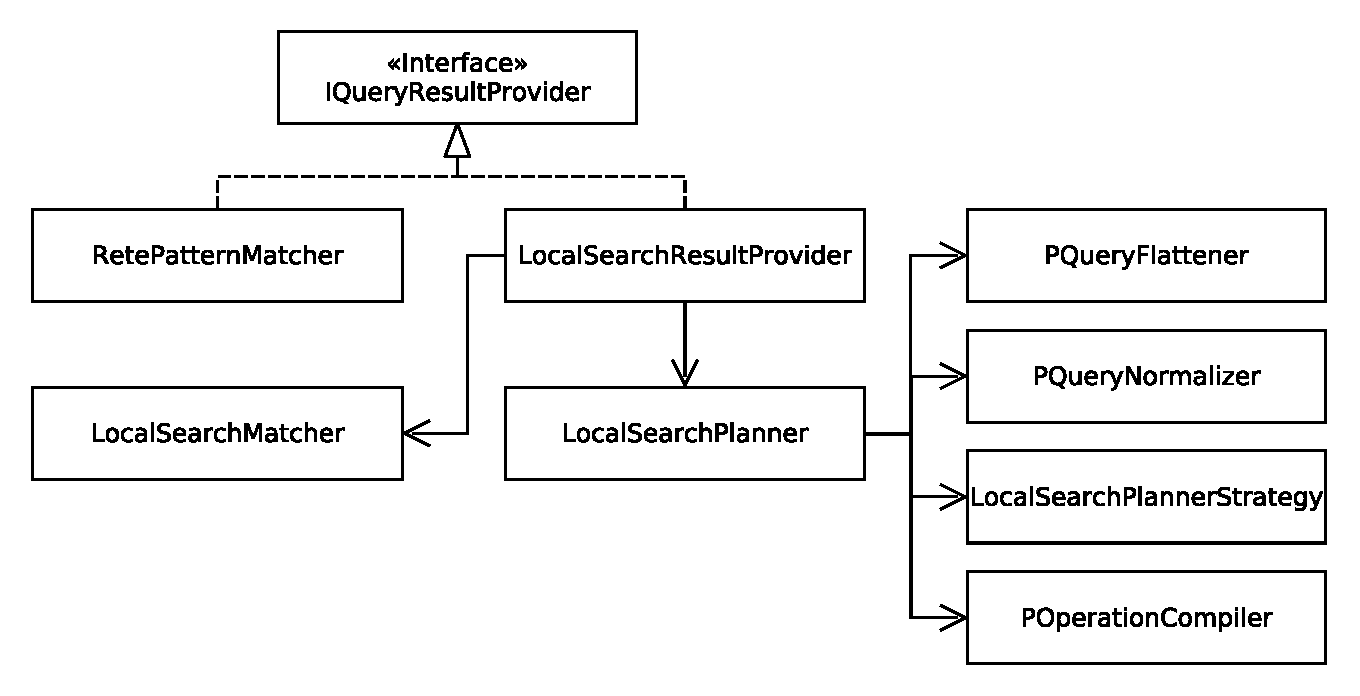
\includegraphics[width=\textwidth]{figures/pdfs/matcher-class-diagram.pdf}
	\caption{The internal structure of the new result provider}
	\label{fig:resultprovider-class}
\end{figure}

We reused the normalizer from the Rete algorithm. The other three components, which also realize steps of the search plan calculation workflow, are created with respect to modularization. Each provide a functionality that may be later replaced with a new implementation. This is especially true for the \texttt{LocalSearchPlannerStrategy}. It holds the business logic for the search plan calculation, so if an alternative version is to be created, only this component should be replaced or changed. 



\subsection{Flattening}
\label{sec:flattening}
 
 The flattening is a novel feature in the \eiq framework. It is not needed by the Rete pattern matcher, but in case of local search-based pattern matching it supports cheaper search plan calculation. Pseudo code of the core algorithm used for flattening is shown in Algorithm~\autoref{alg:flattening}.
 
 
 
 \begin{algorithm}[H]
 	\label{alg:flattening}
 	\caption{Flattening}
 	
 	
 	\SetKwInOut{Input}{input}
 	\SetKwInOut{Output}{output}
 	
 	\SetKwData{PreStack}{preStack}
 	\SetKwData{PostStack}{postStack}
 	\SetKwData{PatternDescription}{patternDescription}
 	\SetKwData{Item}{item}
 	\SetKwData{FlatQueries}{flatBodies}
	\SetKwData{CalledPattern}{calledPattern}

 	
 	
  	\SetKwFunction{Push}{push}
  	\SetKwFunction{Pop}{pop}
  	\SetKwFunction{CopyCalledIntoCaller}{copyCalledIntoCaller}
  	
  
  	\Input{A pattern \PatternDescription}
  	\Output{Semantically equivalent, flattened pattern}
  	
  	\BlankLine
 	
 	\PreStack $ \leftarrow \emptyset $;
 	\PostStack $ \leftarrow \emptyset $; \label{line:init}
 	
 	\PreStack.\Push\functionCall{\PatternDescription}; \label{line:start}

	\While{ \PreStack not empty }{ \label{line:pre-begin}
		\Item = \PreStack.\Pop\functionCall{};
		
		\PostStack.\Push\functionCall{\Item}; \tcp*[f]{Schedule for flattening}
							
		\For{\CalledPattern $\in$ set of patterns called by \Item}{
			\If{\CalledPattern needs flattening} {
				\PreStack.\Push\functionCall{\CalledPattern};  	\tcp*[f]{Fill up \PreStack  \hspace{40pt}}
			}
		}
	}\label{line:pre-end}
	
	\While{ \PostStack not empty }{ \label{line:post-begin}
		\Item = \PostStack.\Pop\functionCall{}; \tcp*[f]{Take out for flattening} \label{line:item-pop}
		
		\Item.\CopyCalledIntoCaller\functionCall{};
	}\label{line:post-end}
	
 \end{algorithm}



In \autoref{line:init} two empty stacks are initialized: \texttt{preStack} holds the patterns that are encountered during the traversal of the call tree, while \texttt{postStack} holds patterns that need to be flattened, and all the referred patterns are flat. In \autoref{line:start} the parameter pattern is scheduled for flattening. To flatten all calls, a \emph{preorder depth-first traversal} is done on the pattern call tree between \autoref{line:pre-begin} and \autoref{line:pre-end}. This collects all calls that are necessary to be flattened at some point. This cycle leaves patterns untouched, only inserts them to the \texttt{preStack} by the time they are encountered during the traversal of the call tree.

From \autoref{line:post-begin} to line \autoref{line:post-end} postorder actions are carried out. At this point we know, that the \texttt{item} in \autoref{line:item-pop} is a pattern that may refer only to flattened patterns, or to patterns that need no flattening. For this reason, the only remaining task is to copy the called patterns into the caller. The function \texttt{copyCalledIntoCaller} leaves the pattern untouched, in case it needs no flattening, in other cases it merges the called pattern constraints and variables to the caller. The reason for this can be the pattern contains no call, or some predicate tells that the pattern should not be flattened.

This algorithm can be used efficiently to flatten pattern calls. However, \eiq has language constructs, for which flattening cannot be applied, namely \texttt{neg find}, \texttt{count find}, and \emph{binary transitive closure}. In these cases the matching should be done by calling matchers for the referenced queries.

A limitation of the current implementation is the lack of support for recursive queries. This algorithm would end up in an infinite loop, if a recursive query was its input. For this reason, in the current implementation the planner first checks for recursion. If the pattern is not recursive, flattener can proceed, otherwise an exception is thrown.

\subsection{Debugger tooling}
\label{sec:lsdebugger}

This description of the Local Search Debugger tooling is from the paper~\cite{DBLP:conf/gg/BurUHV15}. The high-level, declarative nature of graph patterns sometimes results in hard to understand corner cases. In such cases simply looking at match results, as supported by the Query Explorer, does not provide enough details to locate the source of the problem. To support this use case, the development environment of \eiq has been extended with a \emph{Local Search Debugger} view that follows through the execution of a search plan created for a pattern over a model.

As constraints of graph patterns are often not evaluated in the order of their definitions, it is hard to see which constraints are already evaluated during search execution. On the other hand, the ordered search operations visualize the status of pattern matching, and can be traced back to the source pattern. The view can also be used for pattern matching execution optimization, similar to explain plans~\cite{oracle-enterprisemanager} used for optimizing SQL queries.

As \autoref{fig:lsdebugger} depicts a screenshot of the tool. Its view has four distinct parts to display information about as well as to control the execution. At the upper left corner (a) the search plan itself is shown, including the plans created for called patterns. Each line represents a search operation, and child nodes are operations of a called pattern. The current status of the execution is indicated with a set of icons: check marks are assigned to executed operations, question marks are assigned to operations not yet started, while the current operation is denoted with the 'Run' symbol. In this screenshot, the search plan contained in \autoref{tab:catch_flat_normalized_from_debugger} is displayed for the \catchproblem pattern. It is also extended with a final virtual search step called \emph{Match found}, which is only used to visualize the event of finding a match. The execution is halted after the execution of the first three extend operations, and the following check is ready for execution.


\begin{figure}[!htpb]
	\centering
	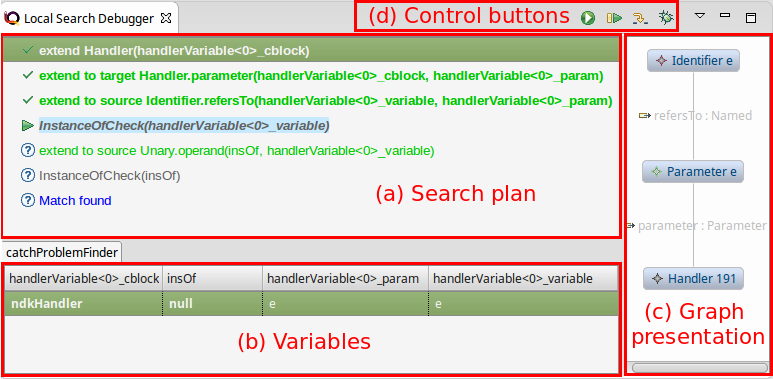
\includegraphics[width=\textwidth]{figures/ls-debugger-tooling}
	\caption{Local search debugger view}
	\label{fig:lsdebugger}
\end{figure}

In the bottom left corner (b) a set of tables is presented on different tabs summarizing the found matches. The tabs have the same name as the corresponding pattern, and the tables include the found matches of all patterns in different tables on different tabs, including both parameters and local variables. In \autoref{fig:lsdebugger}, currently variables \texttt{cBlock}, \texttt{param}, and \texttt{variable} are assigned a value, and \texttt{insOf} is \texttt{null}, which indicates that it is not bound to a value.

In the right side (c) of the view, a graph representation is provided for the currently evaluated (partial) match, showing the current substitutions for the pattern variables along with the relationships between them. The example screenshot depicts that there is an object of type \texttt{Handler} (bottom), which is linked to a \texttt{Parameter} instance (middle). The \texttt{Parameter} instance is further linked to an object of type \texttt{Identifier} (top). The presentation also contains the names and types of objects, and the names of relations.

Finally, to control the execution, (d) standard debugging operations are available~\cite{seifert2008debugging}. Breakpoints can be assigned to search operations either by selecting the operation and clicking on the bug icon, or by double clicking on an operation in the search plan. In addition, both step-by-step and continuous execution modes are available. The former is indicated with the \emph{step into}, the latter is with the \emph{continue halted execution} icon. To initiate the pattern matching process, the play button should be pressed after selecting the desired pattern in the Query Explorer.

This view complements the debugging capabilities of the Query Explorer, as the latter one is useful for identifying problematic cases by providing live feedback when the model changes, while the former visualizes the detailed execution of the search. The local search algorithm, in our experience, works similarly as a query developer reasons about a graph pattern, thus it eases the understanding of complex graph patterns.

%----------------------------------------------------------------------------
\section{Details of search execution}
%----------------------------------------------------------------------------
\label{sec:search-execution}

%Parallelization types: 'level0' and 'level1'
%Figures: visualize the parallelization types

The search execution relies on the search plan to find suitable substitutions for the variables of the pattern. In the following sections a sequential, and a parallel execution approach is introduced in \autoref{sec:sequential-search}, and in \autoref{sec:parallel-search}, respectively.

%TODO{write about environment specific search steps?}

\subsection{Sequential search}
\label{sec:sequential-search}


A generic structure for a search plan is depicted in \autoref{fig:sequential-searchplan}. If an operation is scheduled for th first execution, is \emph{initialized}, then \emph{executed}. A search execution should always start with the initialization of the first operation.


\begin{figure}[!htp]
	\centering
	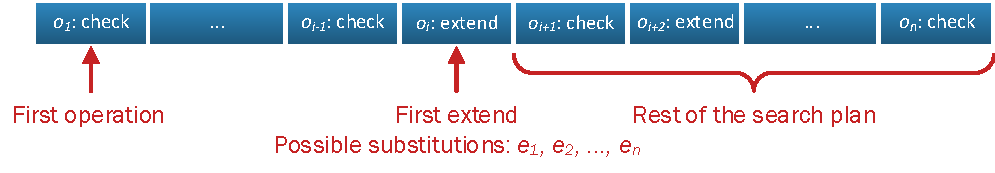
\includegraphics[width=\textwidth]{figures/pdfs/sequential.pdf}
	\caption{Search plan as list of search operations}
	\label{fig:sequential-searchplan}
\end{figure}

For extend operations, the initialization means gathering all elements of a type, or enumerating model elements that are navigable from a reference of a given object. In general terms, it initializes a collection of potential substitutions for a variable. When executing the extend operation, there can be be two outcomes, which are \emph{success} or \emph{failure}. In case of success, the next value from the collection was successfully substituted into a variable. When execution fails, it indicates that there were no more potential substitutions available for the variable.

Initialization for check operations only means setting a boolean indicator \texttt{isExecuted} to \texttt{false}. When the check is executed, it sets \texttt{isExecuted} to true, and the substitutions of the affected variables are tested against the constraint that is assigned to the check operation. The result of the execution returns success, if the substituted values fulfill the requirements set by the constraint and the \texttt{isExecuted} flag was now set to \texttt{true}.

If the execution of an operation is successful, the executor may carry on to the next operation, otherwise it \emph{backtracks}. Upon backtracking, the previous operation is not initialized again, only executed. 

A match is found, when the last operation returns success. In this case, after storing the match, a backtrack is enforced on the last operation in order to find further matches, even though the operation returned success. Matching is finished, when the first operation returns failure.




A running example of the search is illustrated step-by-step in the followings. In this case the search is carried out on the example instance model captured in \autoref{fig:example-instancemodel-handdrawn}, and uses the search plan included in \autoref{tab:catch_flat_normalized}.


\autoref{fig:sst} displays the \emph{search space tree} for the example. Its nodes are symbolizing different states from the aspect of variable bindings. Each of them is represented by a table containing a header with the names of all variables in the pattern, and a single row containing the names of the substituted model elements. The minus sign ($-$) symbolizes that a variable is unbound. The parameter variables are in the left part of the tables, while the right part, which is separated by double vertical lines, holds the rest of the pattern variables.

%, where names are taken from \autoref{fig:example-instancemodel-handdrawn}. 
The directed edges are showing the possible transitions between the states by substituting a suitable value. There are no different states representing fully identical assignments to all variables.


\begin{figure}[!htp]
	\centering
	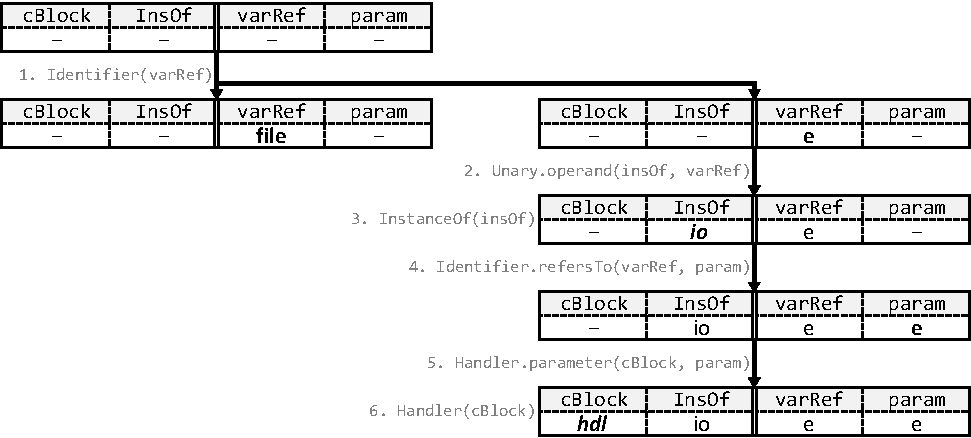
\includegraphics[width=\textwidth]{figures/pdfs/sst.pdf}
	\caption{Search space tree for search plan in \autoref{tab:catch_flat_normalized}}
	\label{fig:sst}
\end{figure}



In our running example, the search starts with unbound variables. In the first step, which is the execution of an extend operation, the executor collects all possible substitutions for \texttt{varRef} in a list, which is in this case \texttt{[file, e]}. Then, it substitutes \texttt{file}, which is the first element, to \texttt{varRef}, and \texttt{proceeds} to the next operation. In \autoref{fig:sst}, the newly substituted values are indicated with bold letters. However, the model does not contain any element of type \texttt{Unary} from which the element \texttt{file} would be navigable via the \texttt{operation} reference, and for this reason the executor \emph{backtracks}.

The next action is to substitute a new value to \texttt{varRef}, which is \texttt{e} with the type \texttt{Identifier}. Then again, the executor seeks for all \texttt{Unary} elements that has \texttt{e} as their \texttt{operand}. This case it gives a list of length 1, namely \texttt{[io]}. Then this only value is substituted to \texttt{insOf}. After substitution, it is made sure that its type is \texttt{InstanceOf} by the check operation, which is indicated by italic letters in the search space tree. Next, the elements of the \texttt{refersTo} relation is gathered, which is a list of containing the model element \texttt{e} of type \texttt{Parameter}, which is not to be confused with the \texttt{Identifier} already substituted to \texttt{varRef}. It is followed by collecting all objects from the model that can reach \texttt{e} via \texttt{parameter} reference. This case it is only the \texttt{hdl}, which is finally checked if it has the type \texttt{Handler}. This is also stands, so a match is found.

At this point the matching process is not over, for all other potential values gathered in extend operations should be tested, if they can form a match. For this reason, the execution backtracks until the last extend operation can pick a new value for substitution. However, this case every extend operations, including the first, have reached to the end of their list of substitution values. For this reason, after the backtracking is done, the pattern matching finishes.

%\todo{a more detailed introduction of search execution}

\subsection{Multi-threaded execution}
\label{sec:parallel-search}
%kb. 3-5 oldal

If a search plan contains at least one extend operation, it means that the executor will test each possible substitutions one-by-one. This provides an opportunity, to distribute the substitution tasks among multiple executors. We proposed a simple solution in which the search plan is forked at the first extend operation. These forks are assigned to separate executors running on different threads in order to harness the additional resources available in multi-core/Hyper-threading computers. The basic idea of the solution is illustrated in \autoref{fig:multithreaded-searchplan}

\begin{figure}[!htp]
	\centering
	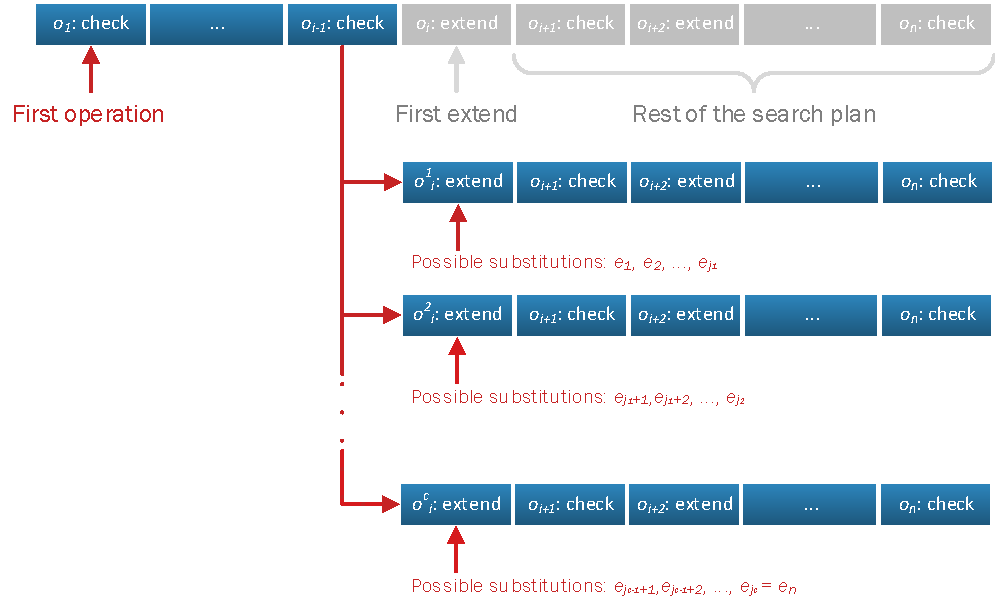
\includegraphics[width=\textwidth]{figures/pdfs/parallel_level1.pdf}
	\caption{A possible parallelization of search plan execution}
	\label{fig:multithreaded-searchplan}
\end{figure}

We can assume that the first extend operation in the search plan is $o_i$ with the possible substitutions $e_1, e_2, \ldots, e_n$, and we also know that $e_p = e_q $ iff $p = q$, where $p,q \in [1,n]$. Then we can evenly distribute the values among $c$ processors by creating $c$ number of modified $o^k_i$ extend operations. These modified extends should have substitution values $e_{j_{k}+1}, e_{j_{k}+2}, \ldots, e_{j_{k+1}}$, where $j_k = (k-1) \cdot \left\lfloor\dfrac{n}{c}\right\rfloor $ for every $k = 1, 2, \ldots, c-1$, and $e_{j_{c}} = n$

Creating a copy of the operations marked as \textit{Rest of the search plan} in \autoref{fig:multithreaded-searchplan} is necessary, because the search operations are represented by stateful objects. Preserving a state is required for extend operations to maintain the internal collection of potential substitutions, and also required for check operations to handle backtracks with the \texttt{isExecuted} flag.

We can summarize our solution for parallelization in three steps:

\begin{enumerate}
	\item The task is to instantiate modified extend operations, marked with the $o^k_i$ in \autoref{fig:multithreaded-searchplan}, and distribute the candidate elements of the first extend among them.  This step also includes creating a copy from the rest of the search plan.
	
	\item Carry out sequential execution for each newly created search plan. Each executor should maintain its own result set, instead putting the matches in a shared collection. The latter option was also considered, but in order to avoid synchronization and blocking, we decided to merge the results in a separate step.
	
	\item Await all executors, then merge the results. The uniqueness of matches is automatically ensured by the fact that the modified extend operations work with disjoint lists of model elements, which is the result of the initial assumption of $e_p = e_q$ iff $p = q$, where $p,q \in [1,n]$.
\end{enumerate}

\subsection{Advantages and weaknesses}
\label{sec:advantages-weaknesses}

A huge advantage of the solution is the possibility to utilize all physical execution cores of the hardware. Based on \emph{Amdahl's law}, using a  CPU with $c$ cores, the time $t$ needed for the sequential \emph{the search execution} could drop to $(1-p) \cdot t + \dfrac{p}{c} \cdot t$, where $p \in [0,1]$ expresses the portion of the instructions that can run in parallel. If there was $ p \approx 1 $, it would yield $\dfrac{t}{c}$ for the new execution time.
This sounds promising, but the evaluation results in  \autoref{sec:performance-evaluation} and in \autoref{sec:performance-evaluation-tb} will show that the speedup in practice is not even close to this bound generally, which means a significant part of the instructions cannot run in parallel.

As a drawback, the solution has preparation overhead. This currently means the creation of the executor thread pool, the distribution of the model elements among executors, and the cloning of the rest of the search plan. Additionally, when creating sublist from the list of elements of the first extend operation, it is unknown how long will it take for the executor, until all matches that involve the element will be found. It may turn out soon that the value fails to fulfill even the constraint associated with the next check, but it is also possible that the substituted value is part of several matches, taking the executor long time to compute them all. 


%----------------------------------------------------------------------------
\chapter{Evaluation}
%----------------------------------------------------------------------------
\label{chap:evaluation}
%Összesen kb. 5-8 oldal

In the current chapter the environment used for assessing the implementation is introduced in \autoref{sec:meas-workflow}, \autoref{sec:meas-env} and in \autoref{sec:meas-patterns}, then the performance of the implemented local search-based pattern matching algorithm is evaluated in \autoref{sec:performance-evaluation}. An additional measurement was done for scalability in an environment with limited memory in \autoref{sec:performance-evaluation-tb}.

%1-2 oldal
\section{Measurement workflow}
\label{sec:meas-workflow}

The measurement setup is composed of four phases: (i) \emph{Read}, (ii) \emph{Create engine}, (iii) \emph{Calculate search plan}, and (iv) \emph{Check}. The steps are depicted in \autoref{fig:measurement-workflow}. 

\begin{figure}[!htp]
	\centering
	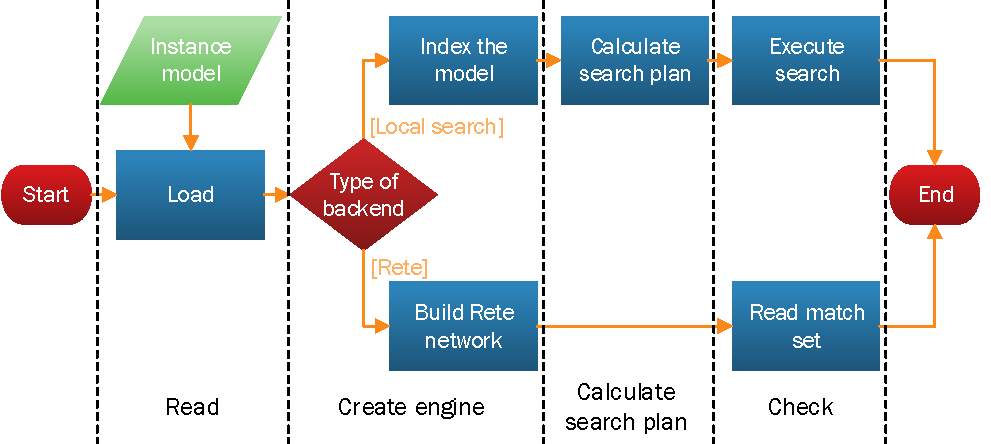
\includegraphics[width=\textwidth]{figures/pdfs/measurement_workflow.pdf}
	\caption{The workflow used for measurements}
	\label{fig:measurement-workflow}
\end{figure}

The Read step measures merely the time needed to load the EMF model into memory. The Create engine step is different for the incremental, and local search-based approaches. For a local search based-algorithm only a basic indexing of the elements is performed in order to provide cardinality information for the search plan calculation. In case of Rete, in addition to the indexing, the whole Rete network is created, which means most of the pattern matching is done here. Calculate search plan phase is only related to local search, for in this step the search plan calculation time is monitored. Finally the time needed for the retrieval of results is observed in the Check phase.


%In this scenario we only assess search execution times executed on a loaded model for the first time. Model modification and re-checking is out of scope, for it means no difference for the local search-based pattern matching.

\section{Measurement environment}
\label{sec:meas-env}

The computer used for carrying out the measurements was a ThinkPad T440p laptop, running Linux 3.16.0-38-generic x86\_64 operating system, and had the following hardware configuration:
\begin{itemize}
	\item CPU: Intel$\circledR$ Core\texttrademark~i7-4700MQ CPU @ 2.40GHz
	\item Memory: 2 $\times$ 4096 MB DDR3 @ 1600 MHz
	\item SSD: Intel 320 Series SSDs, model: INTEL SSDSA2CW160G3
\end{itemize}

We used Java\texttrademark~SE Runtime Environment (build 1.8.0\_66-b17). In order to successfully load every used model to memory, we supplied the JVM 6 gigabytes of heap size by using the \texttt{-Xms6G} and \texttt{-Xmx6G} parameters. 

We tested the performance of the incremental Rete (referred as \emph{Incremental}), the single-threaded local search-based (\emph{Sequential}), and the parallel local search-based (\emph{Parallel}) algorithms. We assessed the performance using the newest algorithm versions available on December 10, 2015 in \eiq.


\section{Models and patterns used for assessment}
\label{sec:meas-patterns}
In order to evaluate scalability of the algorithms, we carried out measurements on three different model sizes with four different queries. Both the models and queries are from~\cite{DBLP:journals/infsof/UjhelyiSHCVVF15}. 

The selected models for this work are the EMF representations of the ASGs of programs \emph{Qwicap}, \emph{Frinika}, and \emph{Hibernate}. Qwicap is a library for Java web application development. Frinika is a music workstation software, which provides several features for editing and working with music. Hibernate is a tool that can be used to implement object-relation mapping for applications to persist data. We chose these softwares, because both are free and open-source, and have different sizes, thus they can help assessing scalability of the approaches. \autoref{tab:model-complexity} summarizes the basic metrics of the source code and the generated ASGs.

% Attributes are not needed for the example queries
%\begin{table}[htbp]
%	\centering
%	\begin{tabular}{c|crrrr}
%		\hline
%		& Version	& LOC		& Node Count 	& Edge Count	& Attribute Count \\
%		\hline
%		
%		Qwicap		 & 1.4b24	& 443 		& 7,903 			& 21,222 		& 59,069 \\			
%		Frinika		 & 0.5.1	& 64,828 	& 429,407 		& 1,292,961 		& 3,065,383 \\		
%		Hibernate	 & 3.5.0	& 773,166 	& 2,444,419 		& 7,563,207 		& 16,789,330 \\	
%		\hline
%	\end{tabular}
%	\caption{Metrics of the analysed ASGs}
%	\label{tab:model-complexity}
%\end{table}

\begin{table}[htbp]
	\centering
	\begin{tabular}{l|crrr}
		\hline
	 Model name& Version	& LOC		& Node Count 	& Edge Count	\\
		\hline

	Qwicap		 & 1.4b24	& 443 		& 7,903 			& 21,222 		\\			
	Frinika		 & 0.5.1	& 64,828 	& 429,407 		& 1,292,961 		\\		
	Hibernate	 & 3.5.0	& 773,166 	& 2,444,419 		& 7,563,207 	\\	
	\hline
	\end{tabular}
	\caption{Metrics of the analyzed ASGs}
	\label{tab:model-complexity}
\end{table}



The four cases if code smell are named \emph{Catch}, which is the same as the example \catchproblem pattern describes, \emph{Constant compare}, \emph{No default switch} and \emph{Unused parameter}. The descriptions of the latter three anti-patterns are again taken from~\cite{DBLP:journals/infsof/UjhelyiSHCVVF15}, and are as follows:

\begin{itemize}
	\item \emph{Constant compare}: When a String variable is compared
	to a String literal using the \texttt{equals()} method, it is unsafe to have the variable
	on the left hand side. Changing the order makes the code safe (by avoiding
	null pointer exception) even if the String variable to compare is \texttt{null}.
	\item \emph{No default switch}: Missing default \texttt{case} has to be added to the \texttt{switch}.
	\item \emph{Unused parameter}: When unused parameters remain in the parameter list
	they can be removed from the source code in most cases.
\end{itemize}

In \autoref{tab:pattern-complexity} we summarized the total number of variables, constraints, and any type of pattern calls used to describe the problem using IQPL. These numbers does not provide precise description, however, they tell that these patterns are adequate for performing measurements to test scalability of the approaches from the aspect of pattern complexity. The \emph{No default switch} is considered to be the simplest, while \emph{Unused parameter} the most difficult to match. 

\begin{table}[!htpb]
	\centering
	\begin{tabular}{l|ccc}
		\hline
 Anti-pattern problem & Variables & Constraints & Pattern calls\\
		\hline
 Catch 			& 6 	& 9 	& 1	\\
 Constant compare & 9 	& 10 	& 4	\\
 No default switch & 3 	& 5 	& 1	\\
 Unused parameter & 19 	& 29 	& 9 \\
		\hline
	\end{tabular}
	\caption{Main attributes of the patterns}
	\label{tab:pattern-complexity}
\end{table}


\section{Performance evaluation}
\label{sec:performance-evaluation}
The output of the assessment for the three different models are summarized in \autoref{fig:csmr-measurements}. For detailed numeric results, please refer to \autoref{tab:qwicap}, \autoref{tab:frinika}, and \autoref{tab:hibernate} in the Appendix. Based on the times needed for each task, we obtained multiple conclusions. 


\begin{figure}
	\centering
	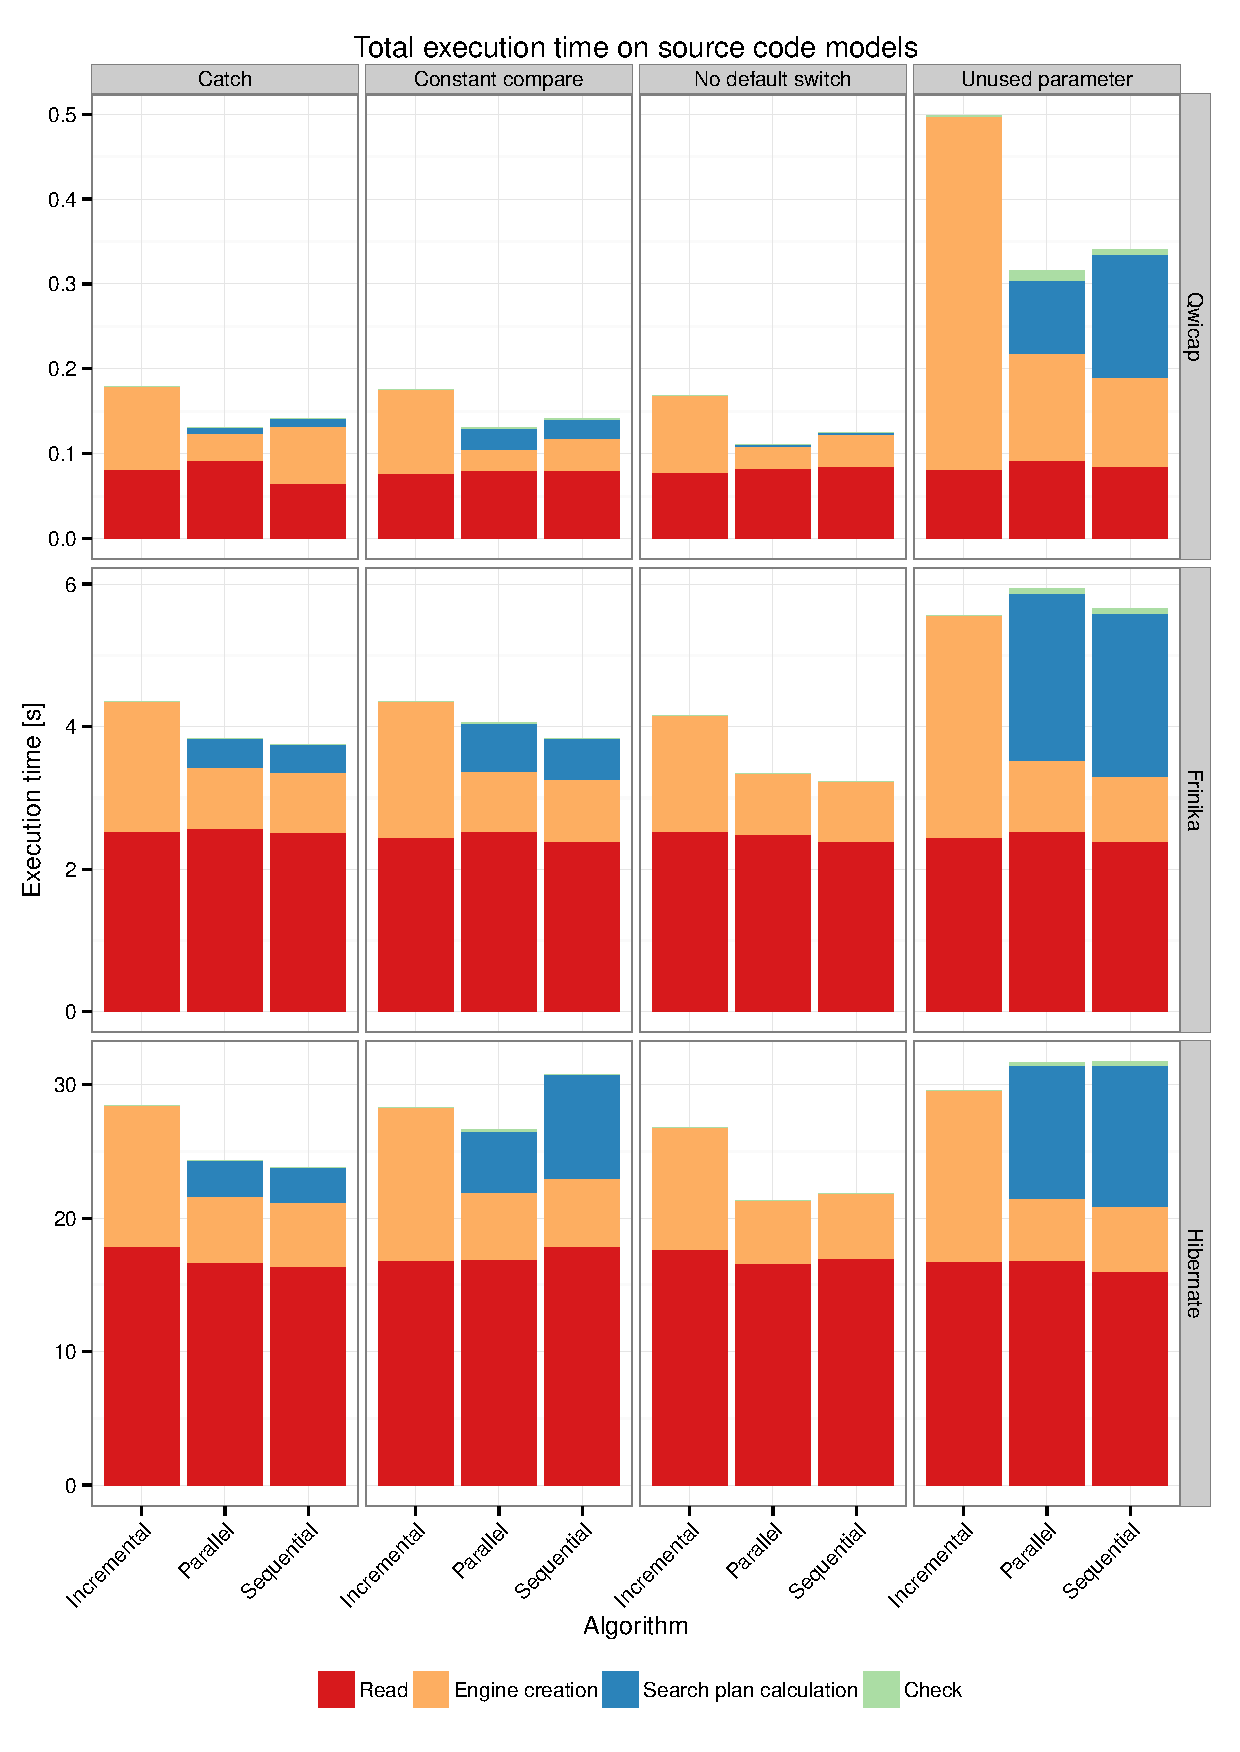
\includegraphics[width=\textwidth]{pdfs/code_model.pdf}
	
	\caption{Measurement results for anti-pattern detection in ASGs}
	\label{fig:csmr-measurements}
\end{figure}


In the Read phase, loading the model takes significant amount of time. In case of large models this is the longest task, but for smaller sizes it is still comparable to engine creation. This complies with the fact that engine creation involves indexing the model elements, and for the Rete algorithm, also building the Rete network based on the index. This also explains why it takes multiple times more, according to the measurements, to finish the engine creation phase for the incremental algorithm.

For the search plan calculation phase, however, unexpectedly large execution times were encountered. This is the step, when the constraints of the pattern are put into an ordered list that makes up the search plan. The current implementation of the algorithm uses cardinality information of types about the instance model in order to determine the order of the operations. After a more detailed analysis of the relevant module, it turned out, that the base indexer has a fairly suboptimal implementation for this part. The method \texttt{countTuples(IInputKey key, Tuple seed)} in \texttt{EMFQueryRuntimeContext} currently returns the result of the \texttt{size()} method called on the result of \texttt{baseIndex.getAllInstances(eClass)}. The already existing implementation of the \texttt{getAllInstances(EClass type)} method of the \texttt{NavigationHelperImpl} class is included in \autoref{lst:getAllInstances}.


\lstset{escapeinside={(*@}{@*)}}
\begin{figure}[!htp]
	\listingjava{getAllInstances}{The implementation of the \texttt{getAllInstances} method}
\end{figure}

This method, as its name advices, returns a collection of all objects of a given type. If we inspect the implementation, in line \autoref{line:newset}, a new \texttt{Set} is instantiated. All subtypes of the given type are collected in line \autoref{line:subtypes}. Between line \autoref{line:subtypes-begin} and line \autoref{line:subtypes-end} all instances of all subtypes are added to \texttt{retSet}, if there were any. In line \autoref{line:instances} all direct instances of the given type are added to the set containing the collected subtype instances. Finally, in \autoref{line:return} \texttt{retSet} is returned. According to our measurements, adding approximately 100,000 elements to an empty set, then calling \texttt{size()} takes about $20$~ms on the computer, on which the performance evaluation was carried out. For these cardinality information are not cached, if it is needed multiple times, the same gathering of elements is carried out again. It also turned out, that the planner in many cases does ask for cardinality information several times for a type.

An important observation is that generally the execution of Check phase may require orders of magnitude less time than other steps. In case of the Rete algorithm this step consists of only returning a copy of a collection in which matches are stored, because it is already prepared by the time the Rete network is built. The local search-based algorithm, however, computes the matches in this final phase of measurement. Thanks to the efficient, model sensitive search plan, which is calculated in the preceding phase, the search for matches is done under a few milliseconds for most cases. We experienced slightly notable durations for the largest used model, Hibernate. In this case the matcher for \emph{Constant compare} and \emph{Unused parameter} patterns worked several hundred milliseconds to compute matches. It is also important to add, that these patterns are considered to be more complex than \emph{Catch} and \emph{No default switch}.

The results also shed light on the shortcomings of the current search parallelization. The implementation creates a thread pool with $c$ threads, where $c$ equals the number of currently available cores of the CPU. Then, the parallelization starts when the search execution reaches the first extend operation, where the potential substitutions are divided between the threads. The creation of a thread pool and distributing the work among threads seemingly imposes some overhead, as it was foreseen in \autoref{sec:advantages-weaknesses}. 

%Also, as it was covered in \autoref{sec:advantages-weaknesses}, at the point of substitution of a value it is not known, how much time will it take to calculate all possible matches. For this reason the distribution of the values among threads may cause uneven workload among executors. However, to get all results all executor thread should finish to be able to create a unified collection of matches.

To decide which algorithm should be used in a certain scenario depends on several circumstances. According to the results, we can estimate the number of runs, where the Rete algorithm outperforms the local search-based one in runtime. If we were to match the \emph{Catch} problem against the model \emph{Frinika} only once, it would take $2.535 + 1.813 + 0 + 0.0017 = 4.3497$~seconds with the incremental algorithm. The same scenario would took $ 2.512 + 0.842 + 0.400 + 0.0009 = 3.7549 $~seconds for the sequential local search-based algorithm. However, if we increased the number of runs on a loaded model with an already created engine, each additional run after the first one would took only $ 0.0017 $~seconds with Rete, and $ 0.4009 $~seconds with the current implementation of the sequential local search-based version. From these data, we can obtain a run count threshold, for which incremental algorithm is more beneficial with respect to execution time. This run threshold $r$ comes from the equation 
$$ 2.535 + 1.813 + r \cdot 0.0017 = 2.512 + 0.842 + r \cdot (0.400 + 0.0009), $$
and it yields $ r \approx 2.5 $. So it means, if we run the same anti-pattern detection several times on the model only one or two times, it is worth using local search, in other cases Rete will finish faster. If we apply the above calculations for the measurement results of \emph{No default switch}, we get a threshold $r \approx 1546.7$. However, we have to remark three important factors regarding the above calculations:

\begin{itemize}
	\item Rete network update times are neglected in this calculation, for they are assumed to be minimal for small model changes.
	\item Currently the search plan calculation is highly ineffective due to a shortcoming in the implementation of the base indexer. If this problem were fixed, the time needed for plan calculation for local search would notably drop.
	\item In these cases the memory bounds were not a limitation.
	\item Search plans are not cached for later execution.
\end{itemize}

\section{Running the Train Benchmark}
\label{sec:performance-evaluation-tb}

Train Benchmark is a benchmarking framework aiming to test query evaluation performance of model-driven engineering tools~\cite{trainbenchmark}. This evaluation is carried out by matching the same patterns against several models with growing sizes. For this purpose Train Benchmark has a model generator component that creates synthetic models for a given size range. It also provides predefined patterns to match against the generated models, for which basic complexity information are included in \autoref{tab:tb-pattern-complexities}. For detailed description of the models provided by the generator and the patterns, please refer to the cited technical report above.


 \begin{table}[ht]
 	\centering
 	\begin{tabular}{l|ccc}
 		\hline
 		Pattern & Variables & Constraints & Pattern calls \\
 		\hline
		 ConnectedSegments & 7 & 7 & 0 \\
		 RouteSensor & 4 & 4 & 1 \\
		 SemaphoreNeighbor & 7 & 8 & 1 \\
		 SwitchSet & 4 & 7 & 0 \\
 		\hline
 	\end{tabular}
 	\caption{Train Benchmark pattern names and complexities}
 	\label{tab:tb-pattern-complexities}
 \end{table}



In our case we used this framework to test the scalability of the pattern matching algorithms on the benchmark scenario depicted in \autoref{fig:measurement-workflow}. We ran these measurements on a virtual machine with the following hardware configuration:

\begin{itemize}
	\item CPU: Intel$\circledR$ Xeon$\circledR$ CPU E5-2630L v2 @ 2.40GHz (12 cores)
	\item Memory: 32 GB DDR3 @ 1600 MHz
	\item SSD: Intel Corporation 82371SB PIIX3 IDE [Natoma/Triton II]
\end{itemize}

We used Java\texttrademark~SE Runtime Environment (build 1.8.0\_66-b17), and ran the JVM without extra parameters, which means the heap size limit was 1 GB.

Benchmarking memory consumption is a non-trivial issue in case of managed environments like Java. For this reason we chose a limit for the maximum heap size. From this limit we will not know the exact amount of memory needed, an \emph{out of memory error} can indicate that the program could not fit in the available size. This strategy can be used to decide which algorithm needs more memory than others.

The performance characteristics were similar to what we described previously in \autoref{sec:performance-evaluation}. The search plan generation times for the patterns of Train Benchmark, depicted in \autoref{fig:tb-calc-search-plan}, were increasing with model size (in the diagram both axes are logarithmic). This also leads to the conclusion that obtaining type cardinality information depends on model sizes. The diagram also shows that search plan calculation for different patterns for the same model size take time based on the complexity of the pattern.


\begin{figure}[htpb]
	\centering
	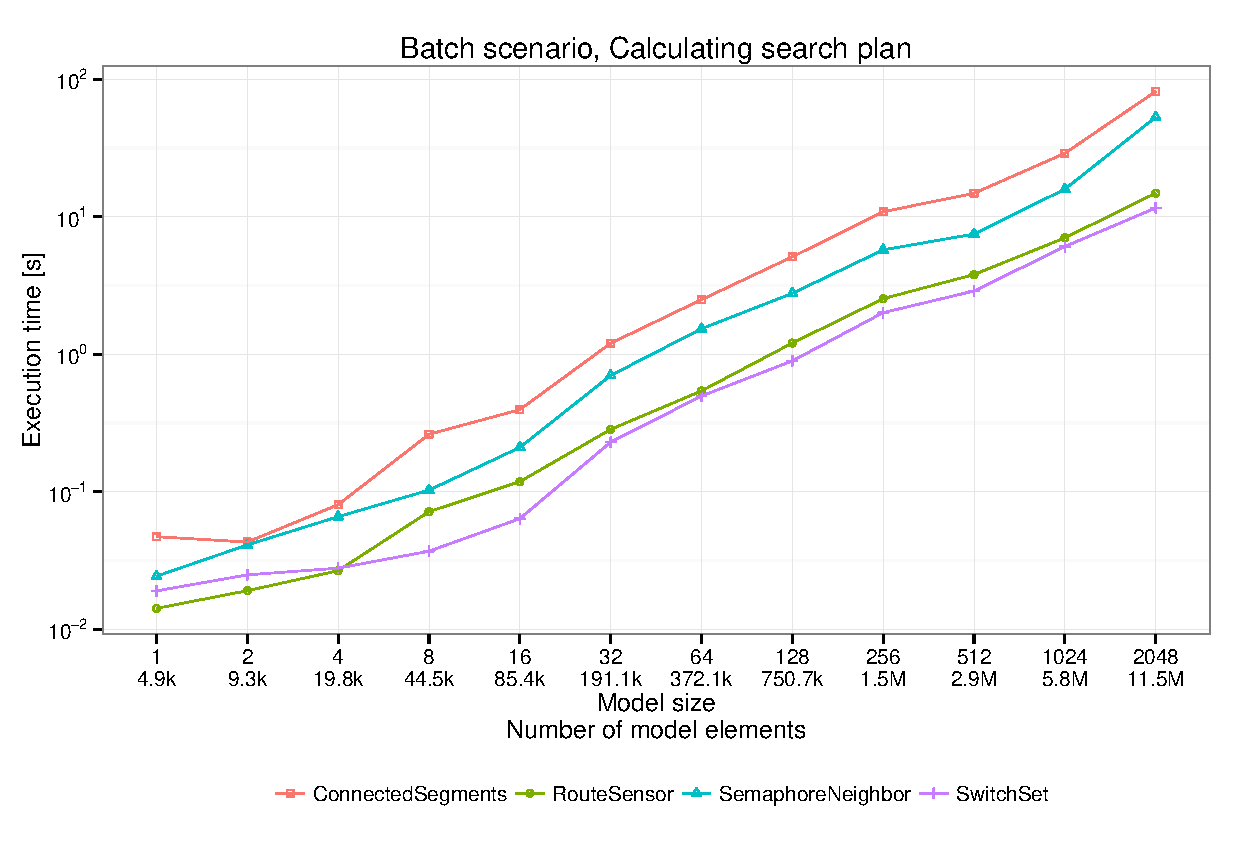
\includegraphics[width=\linewidth]{pdfs/Batch-Calculating-search-plan.pdf}
	
	\caption{Search plan calculation times for different patterns}
	\label{fig:tb-calc-search-plan}
\end{figure}

On the synthesized models of Train Benchmark, we measured mostly linear characteristics for both the sequential and the parallel local search-based pattern matching. The results are depicted in \autoref{fig:tb-check} (again, note the logarithmic axes in the diagram). In this cases, we can observe almost immediate retrieval of results in case of Rete for every pattern. However, for the local search based-pattern matching solutions both scale up in a linear way with the model sizes. We can see that the parallel version of the implementation has an overhead compared to the sequential solution, by comparing the check times needed for small model sizes. This overhead, however, may pay off, since in case of large models the parallel version completes faster.

The benchmark also showed that the incremental algorithm is more constrained by memory than local search-based approaches. While running the benchmark with \emph{ConnectedSegments} on model scale 2048, the measurement was terminated by an out of memory error, showing that the Rete network grew too large in this case.

\begin{figure}[htpb]
	\centering
	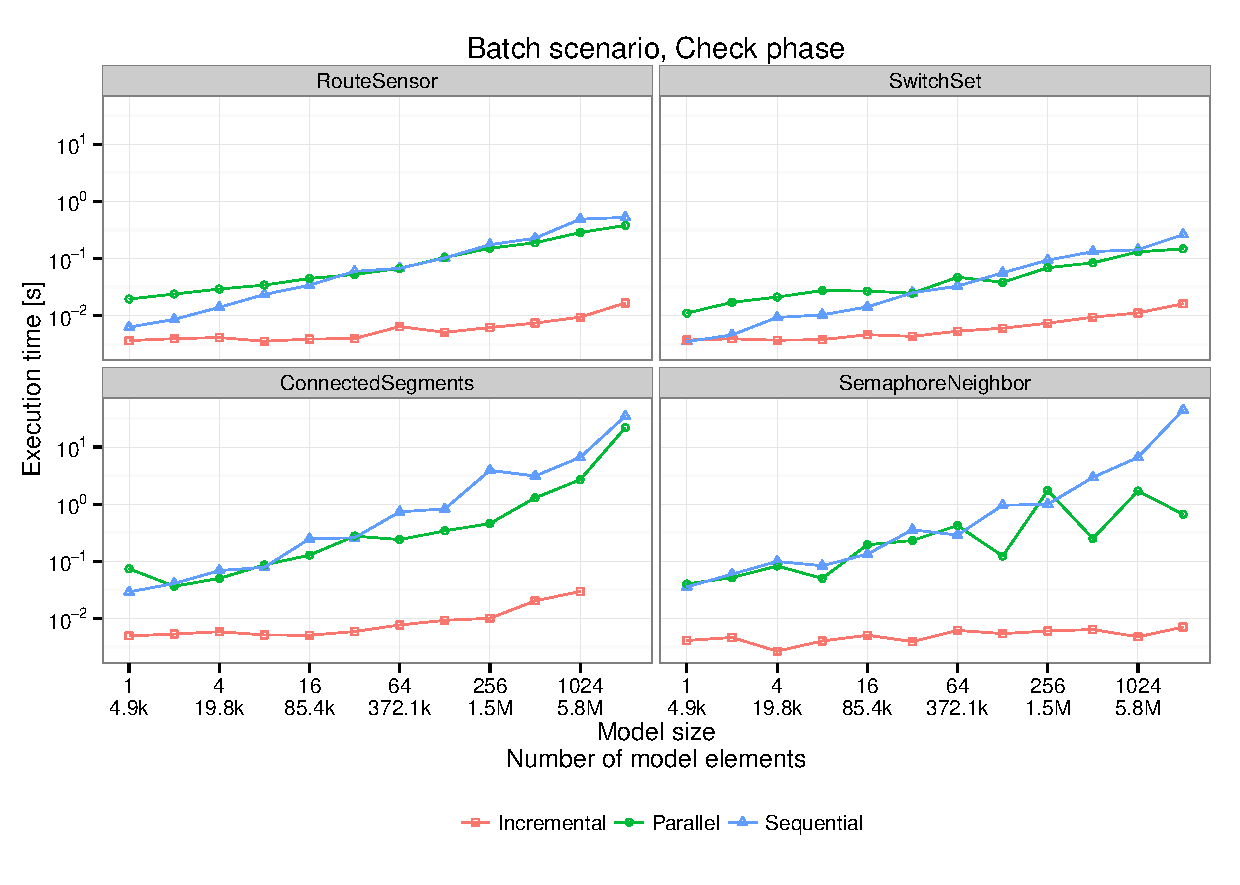
\includegraphics[width=\linewidth]{pdfs/Batch-Check-phase.pdf}
	\caption{Times needed for the Check phase}
	\label{fig:tb-check}
\end{figure}


The rest of the diagrams and tables, which contain the evaluation results of the benchmark, are included in \autoref{appendix:trainbenchmark-results} in the Appendix.

\section{Evaluation summary}

Based on the performed measurements, we came to the conclusion that the \emph{incremental Rete algorithm} runs significantly slower for the first time, compared to the implemented local search-based approach. It also requires more memory for execution. However, we recommend to use this algorithm despite these extra requirements if the same pattern should be matched against the model multiple times consecutively, and if sufficient amount of memory is available.

The sequential local search-based solution has lower memory requirement in many cases, compared to Rete. If the pattern matching is a one-time task, and the cardinality information about the model elements is available, then this is the recommended algorithm.


The parallel local search-based approach differs from the sequential version only in search execution. It has an initial overhead, but for large models it is more preferable in cases where local search should be used.

%2 oldal


%\begin{figure}
%	\centering
%	\subfloat{%
%		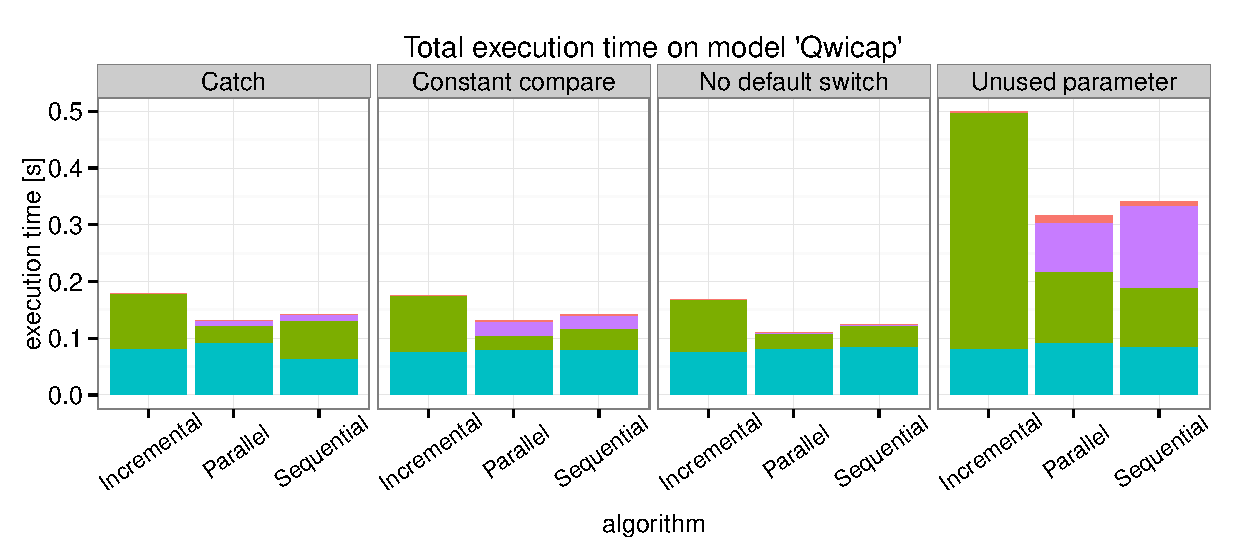
\includegraphics[width=\linewidth]{pdfs/qwicap_resized.pdf}
%	}\par
%	\subfloat{%
%		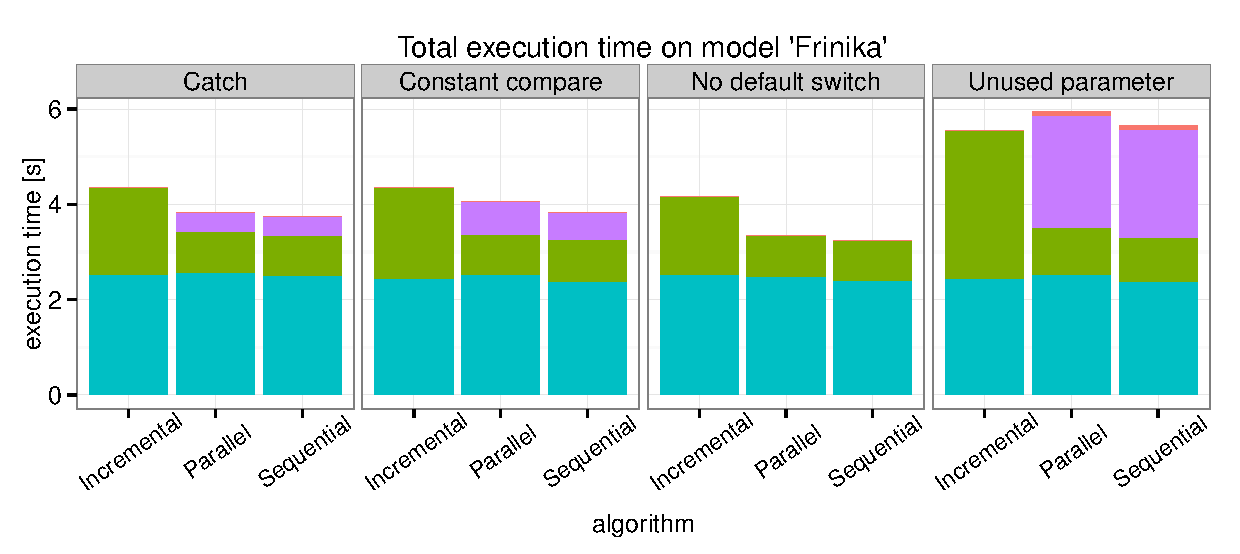
\includegraphics[width=\linewidth]{pdfs/frinika_resized.pdf}
%	}\par        
%	\subfloat{%
%		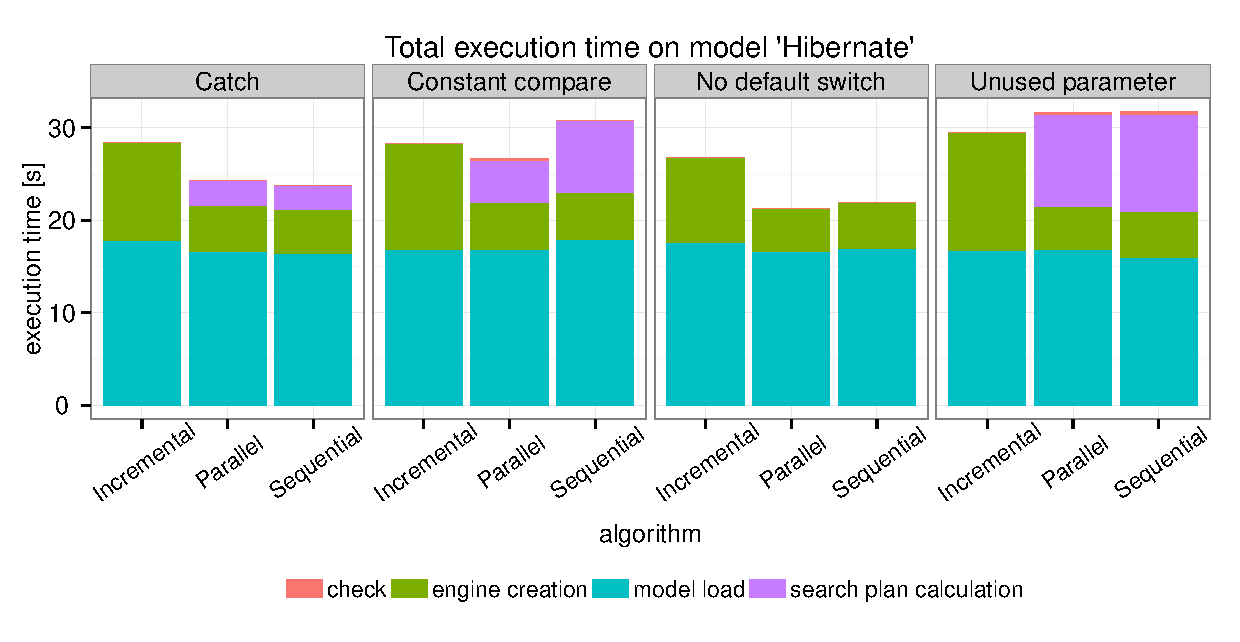
\includegraphics[width=\linewidth]{pdfs/hibernate_resized.pdf}
%	}
%	\caption{Measurement results for anti-pattern detection in ASGs}
%	\label{fig:csmr-measurements}
%\end{figure}




%\clearpage
%\begin{figure}[hp]
%	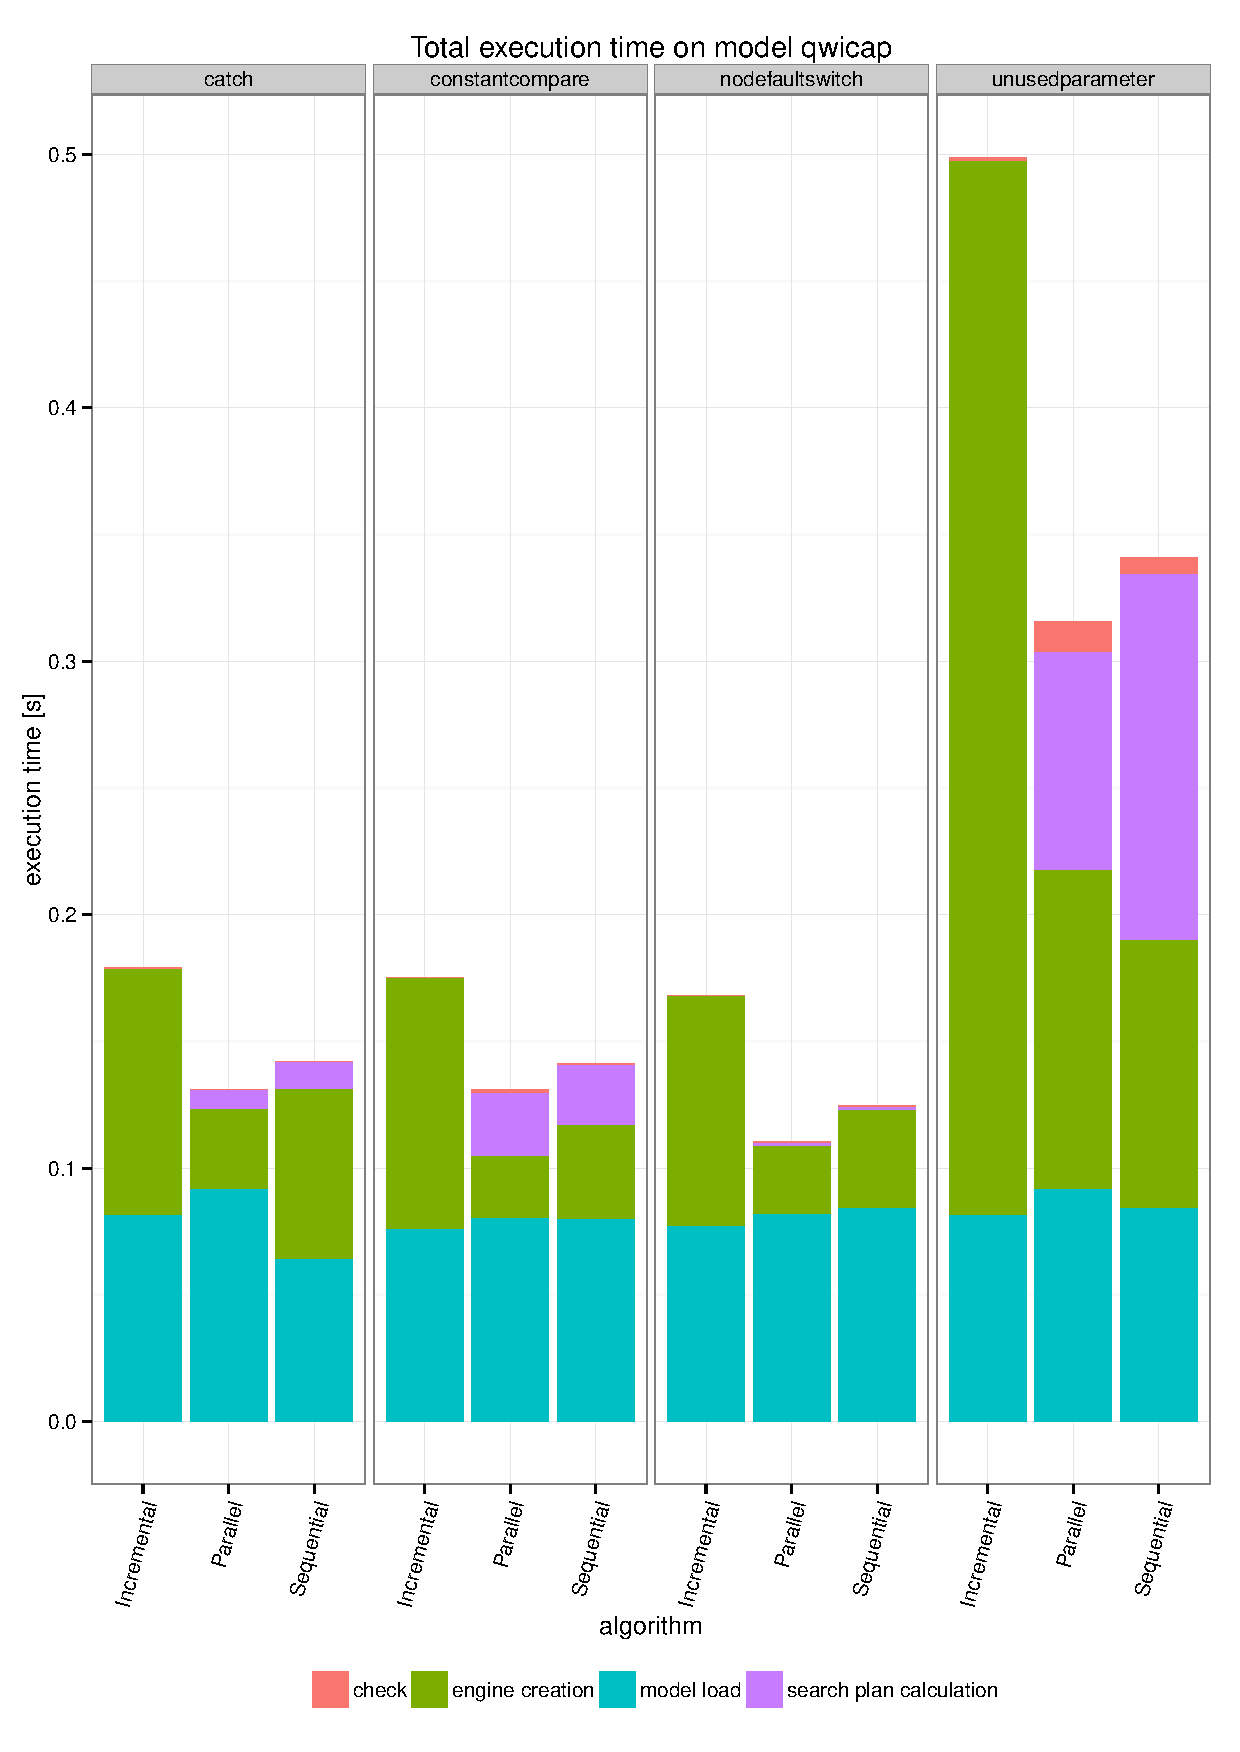
\includegraphics[width=\linewidth]{pdfs/qwicap.pdf}
%\end{figure}
%\begin{figure}[hp]
%	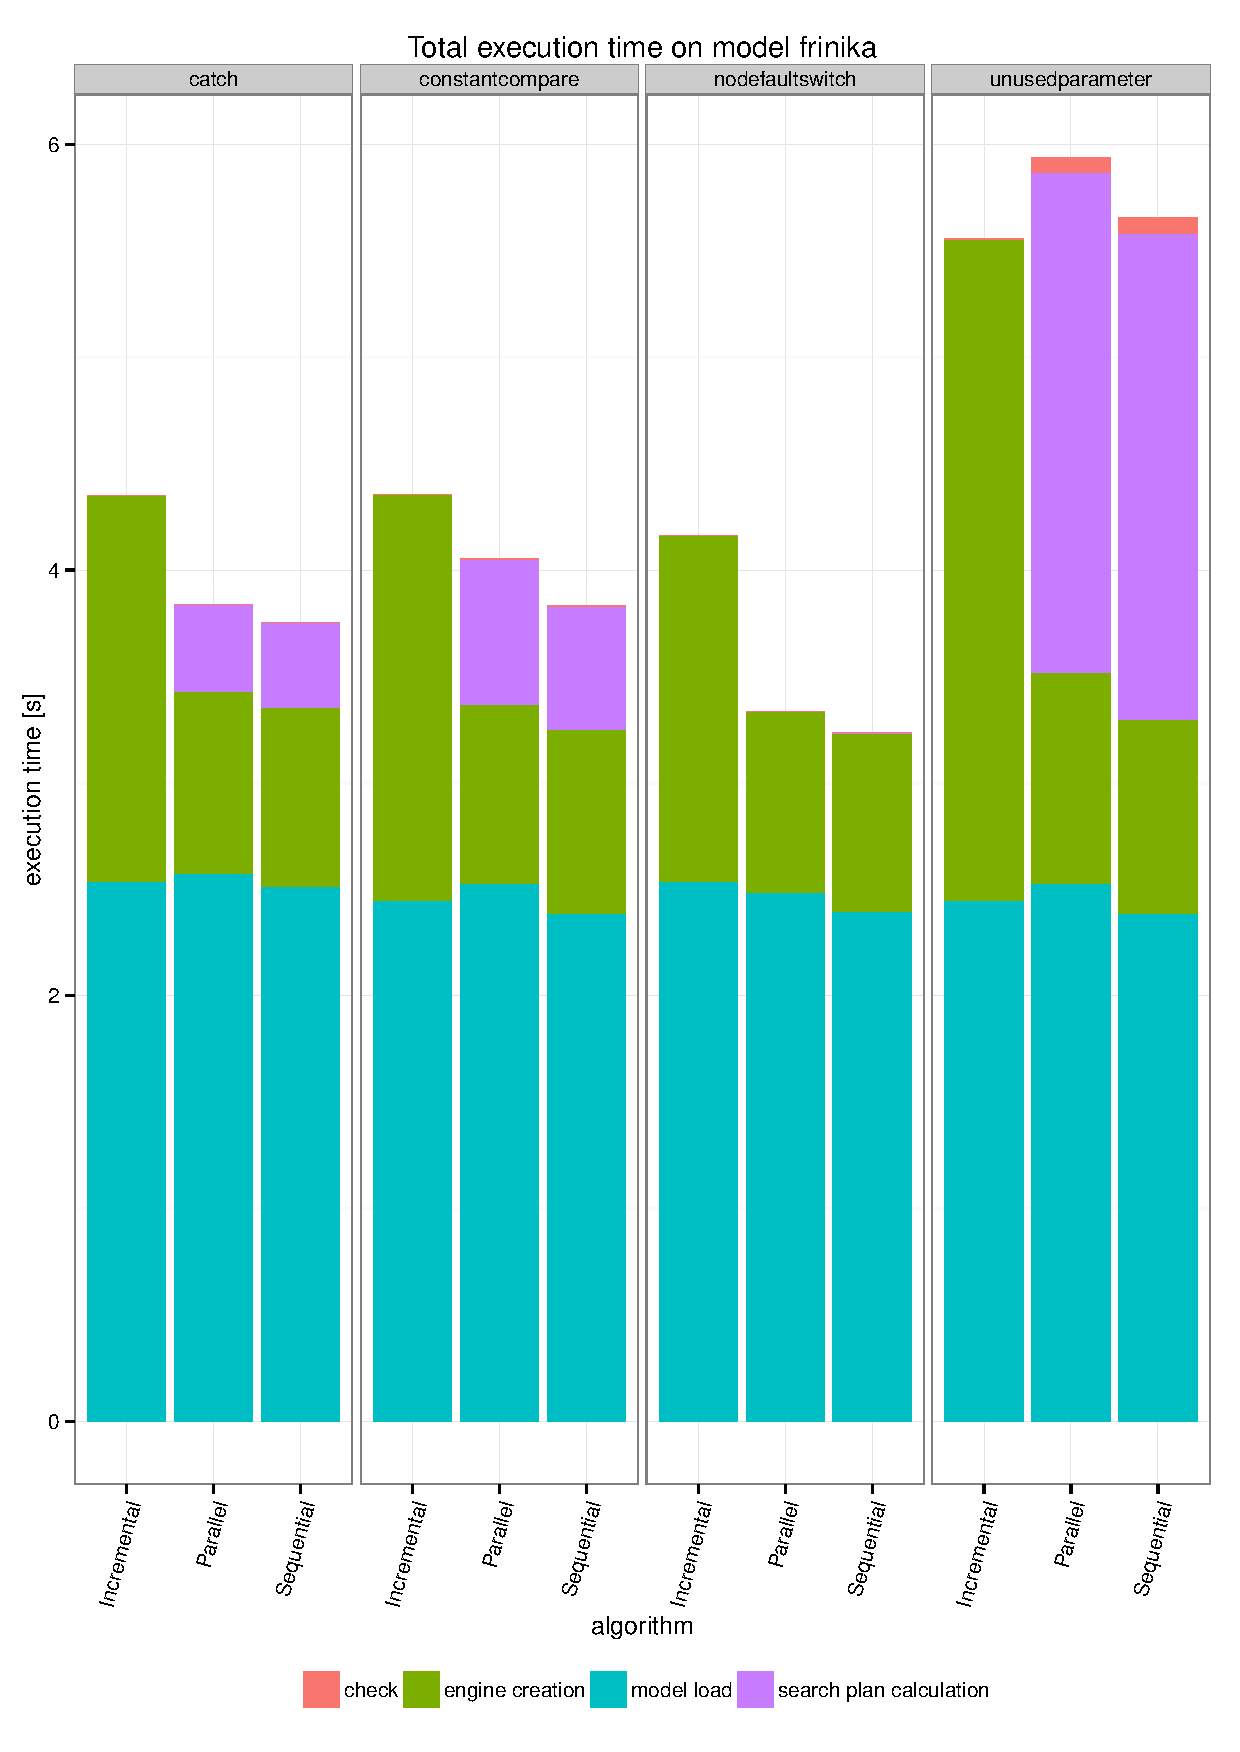
\includegraphics[width=\linewidth]{pdfs/frinika.pdf}
%\end{figure}
%\begin{figure}[hp]
%	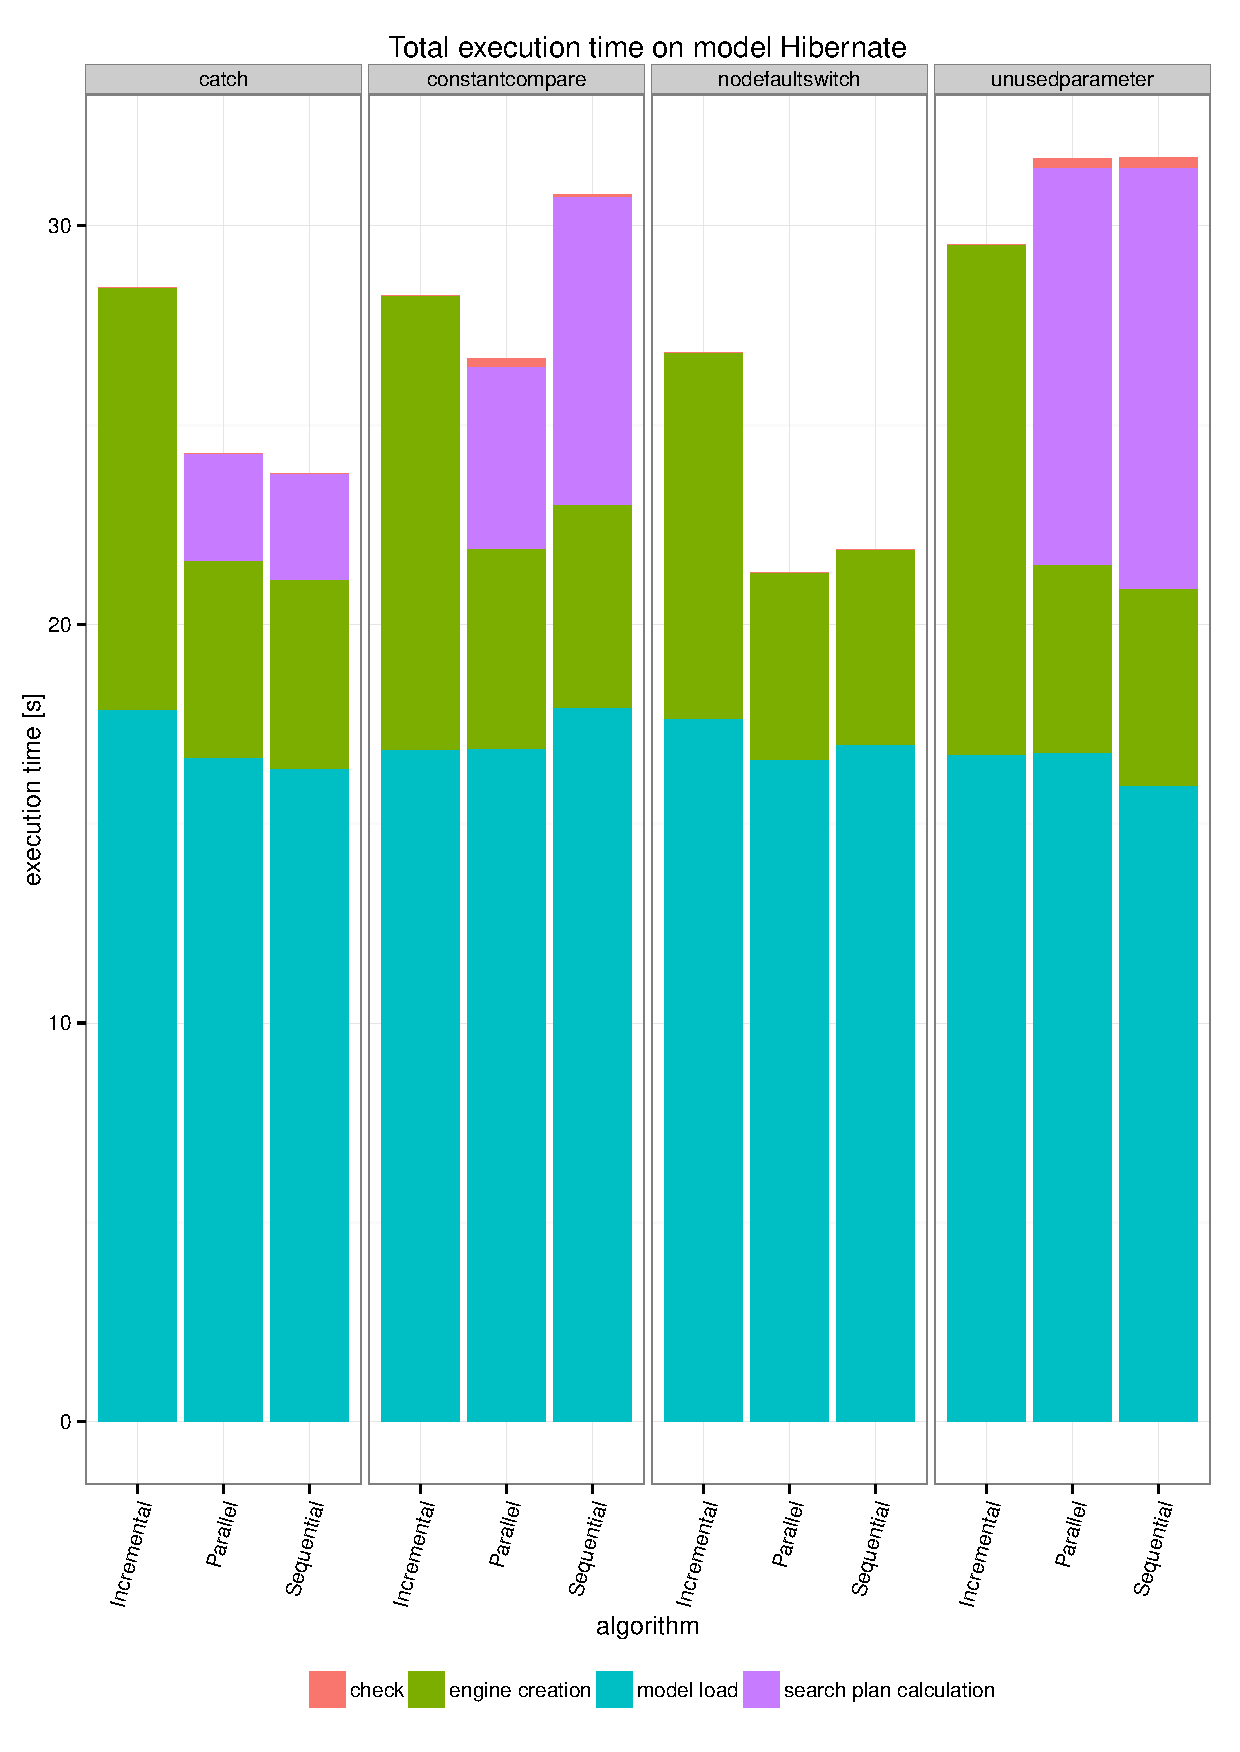
\includegraphics[width=\linewidth]{pdfs/hibernate.pdf}
%\end{figure}
%%----------------------------------------------------------------------------
\chapter{Related work}
%----------------------------------------------------------------------------

%----------------------------------------------------------------------------
\chapter{Conclusion and future work}
%----------------------------------------------------------------------------
\label{chap:conclusion}

%Összesen ~3 oldal


%----------------------------------------------------------------------------
\section{Conclusions}
%----------------------------------------------------------------------------

%In our work we introduced the basics of graph pattern matching along with the motivation for solving such problems. 

We implemented and integrated to the \eiq framework a model adaptive search plan calculation algorithm for local search-based pattern matching. We also provided two search execution runtimes, a single-threaded and a simple parallel runtime. 

The implementation was tested for performance and scalability, and was compared to an already existing, incremental pattern matching algorithm from the aspect of execution time. This evaluation, and comparison was done for models coming from two different domains. First part of the measurements were done on source code models with patterns describing program code smells. Additionally, we used the Train Benchmark to assess the usability of the proposed solution. The results proved that in scenarios, in which patterns are only matched against a model.

We also provided tooling support for the local search algorithm with a Local Search Debugger component, which can help programmers find problems with the pattern definitions, and provide help in finding time consuming operations in the pattern matching process.

%----------------------------------------------------------------------------
\section{Summary of contributions}
%----------------------------------------------------------------------------

I successfully adapted a local search-based pattern matching algorithm, which involves a model sensitive local search planner implementation, and two executor runtimes. During the implementation solved several design issues and integrated the result to the open-source \eiq project. I provided support for debugging the local search execution by the Local Search Debugger View. 

I assessed the performance and scalability of the solutions, and via the evaluation I showed that the local search-based algorithm provides a scalable solution for pattern matching even over large models. The measurements also shed light on a shortcoming of the current implementation of the \eiq Base Indexer.



%----------------------------------------------------------------------------
\section{Future plans}
%----------------------------------------------------------------------------

The ultimate goal of the \eiq graph pattern matching framework is to successfully, and efficiently find matches of a pattern over a given model. To improve execution times of the local search based approaches, there are several improvement possibilities.

\subsection{Information about type cardinality}
It was covered in \autoref{sec:performance-evaluation} that the current implementation of the base indexer is suboptimal. In addition to optimizing the current implementation, the performance can be improved by providing an option to only maintain type cardinalities. This could return the required information with minimal overhead in execution time. It would also take up less memory than the current implementation of the base index, for it would not keep track of the model elements themselves, only just the number of instances of the types. This information is sufficient in most cases, when inverse navigation along links is not a requirement.

\subsection{Adaptive cost calculation}
The search operation costs are calculated based on the instance model properties, type of the corresponding constraint, and the types of operations, which can be extend or check. This, however, is still an estimation for the time needed to execute the operation. For this reason, this information may mislead the local search planner, when an expensive operation is declared to be cheap by the cost function. 

The times needed for operations to execute can be collected runtime. We suppose that by analyzing the historical data about the execution times can significantly help search operation cost estimation by assigning different kinds of bias to search operations that take a long time to finish.


\subsection{Advanced parallel execution}
%TODO work stealing

As it was emphasized in \autoref{sec:advantages-weaknesses}, the current parallel pattern matching execution runtime relies on a basic concept, and may not result in significant speedup. The evaluations show that on practical models, in our case obtained from software source code, this approach does not seem to be successful. In case of artificial models, a tendency was discovered that for larger sizes the parallel outperforms the sequential implementation, but the execution times are far below the theoretic possible speedup.

In order to approach the desired execution time introduced also in \autoref{sec:advantages-weaknesses}, \emph{work stealing} should be applied. This would mean that at any point of the search plan, the matching process could be forked by several sequential executors. In an ideal case, this would happen in an on-demand way during search execution: if an executor seems to have significantly more work at a given extend operation, while other executors have finished their part, the work could be redistributed, thus the computational resources of the platform could be harnessed again.

\subsection{Hybrid pattern matching}

In the \eiq framework there are two available graph pattern matching strategies for the users, and both approaches has their own advantages and drawbacks. It would be beneficial, to allow their combination in order to profit from their advantages. To accomplish this, we see the following options. (i) Local search based pattern matcher may call incremental pattern matchers for calculating matches of calls. (ii) In case of a Rete matcher, the production representing a called pattern can be provided by the result set of a local search-based matcher.

% Acknowledgements
%~~~~~~~~~~~~~~~~~~~~~~~~~~~~~~~~~~~~~~~~~~~~~~~~~~~~~~~~~~~~~~~~~~~~~~~~~~~~~~~~~~~~~~
%----------------------------------------------------------------------------
\chapter*{\koszonetnyilvanitas} % \addcontentsline{toc}{chapter}{\koszonetnyilvanitas}
%----------------------------------------------------------------------------

Firstly, I would like to express my sincere gratitude to my advisors, Ákos Horváth and Zoltán Ujhelyi for their continuous support and invaluable advices throughout my work.

Besides my advisors, I thank Gábor Szárnyas for all the precious help with the Train Benchmark framework, and data visualization.

Finally, I would like to thank the staff working for DigitalOcean for providing me a multi-core virtual machine to run Train Benchmark.



% List of Figures, Tables
%~~~~~~~~~~~~~~~~~~~~~~~~~~~~~~~~~~~~~~~~~~~~~~~~~~~~~~~~~~~~~~~~~~~~~~~~~~~~~~~~~~~~~~
\listoffigures\addcontentsline{toc}{chapter}{\abrakjegyzeke}
\listoftables\addcontentsline{toc}{chapter}{\tablazatokjegyzeke}


% Bibliography
%~~~~~~~~~~~~~~~~~~~~~~~~~~~~~~~~~~~~~~~~~~~~~~~~~~~~~~~~~~~~~~~~~~~~~~~~~~~~~~~~~~~~~~
\bibliography{bib/mybib}
\addcontentsline{toc}{chapter}{\irodalomjegyzek}


% Appendix
%~~~~~~~~~~~~~~~~~~~~~~~~~~~~~~~~~~~~~~~~~~~~~~~~~~~~~~~~~~~~~~~~~~~~~~~~~~~~~~~~~~~~~~
%----------------------------------------------------------------------------
\appendix
%----------------------------------------------------------------------------
\chapter*{\fuggelek}\addcontentsline{toc}{chapter}{\fuggelek}
\setcounter{chapter}{\appendixnumber}
%\setcounter{equation}{0} % a fofejezet-szamlalo az angol ABC 6. betuje (F) lesz
\numberwithin{equation}{section}
\numberwithin{figure}{section}
\numberwithin{lstlisting}{section}
%\numberwithin{tabular}{section}

%----------------------------------------------------------------------------
\section{A more detailed metamodel for program ASGs}
%----------------------------------------------------------------------------

This metamodel fragment in \autoref{fig:example-extended-mm} contains all types required for the example instance model in \autoref{fig:example-instancemodel-handdrawn}.

\begin{figure}[!htp]
	\centering
	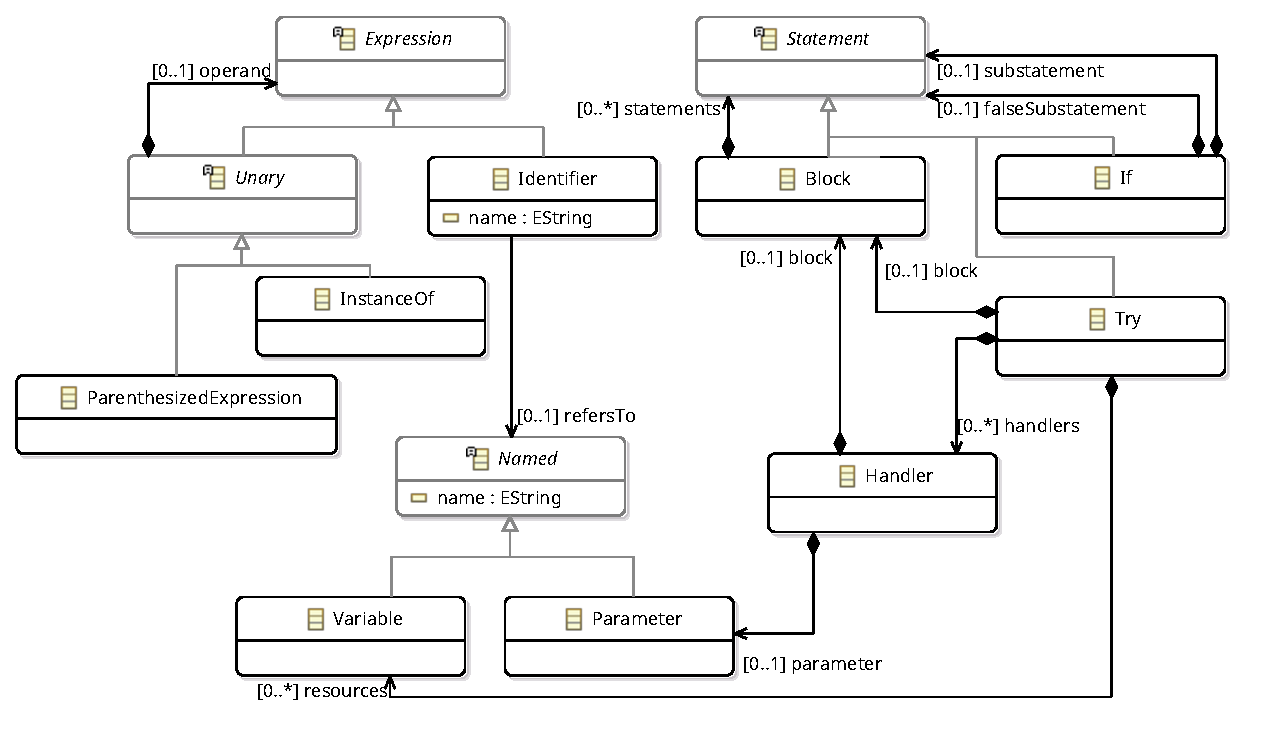
\includegraphics[width=\textwidth]{figures/pdfs/example-metamodel-extended-edited.pdf}
	\caption[~A more detailed EMF metamodel fragment for ASGs]{A more detailed EMF metamodel fragment for ASGs}
	\label{fig:example-extended-mm}
\end{figure}



%----------------------------------------------------------------------------
\clearpage\section{Detailed measurement results for code anti-patterns}
%----------------------------------------------------------------------------
\label{appendix:csmr-results}

Numeric output of the measurement process on the source code examples by phases is displayed in \autoref{tab:qwicap}, \autoref{tab:frinika}, and \autoref{tab:hibernate}.


%\clearpage
% latex table generated in R 3.2.2 by xtable 1.8-0 package
% Sun Dec 13 02:05:38 2015
\begin{table}[!htb]
	\centering
	\begin{tabular}{rllrrrr}
		\hline
		& Case & Tool & Read & \shortstack{\\Create\\engine} & \shortstack{Calculate\\search plan} & Check \\ 
		\hline \hline
		1 & Catch & Incremental & 0.082 & 0.097 & N/A & 0.0002 \\ 
		2 & Catch & Parallel & 0.092 & 0.032 & 0.008 & 0.0000 \\ 
		3 & Catch & Sequential & 0.064 & 0.067 & 0.010 & 0.0001 \\ 
		\hline
		4 & Constant compare & Incremental & 0.076 & 0.099 & N/A & 0.0002 \\ 
		5 & Constant compare & Parallel & 0.081 & 0.025 & 0.025 & 0.0014 \\ 
		6 & Constant compare & Sequential & 0.080 & 0.037 & 0.023 & 0.0007 \\ 
		\hline
		7 & No default switch & Incremental & 0.077 & 0.091 & N/A & 0.0001 \\ 
		8 & No default switch & Parallel & 0.082 & 0.026 & 0.001 & 0.0004 \\ 
		9 & No default switch & Sequential & 0.085 & 0.038 & 0.001 & 0.0002 \\ 
		\hline
		10 & Unused parameter & Incremental & 0.082 & 0.416 & N/A & 0.0013 \\ 
		11 & Unused parameter & Parallel & 0.092 & 0.126 & 0.086 & 0.0120 \\ 
		12 & Unused parameter & Sequential & 0.084 & 0.106 & 0.144 & 0.0063 \\ 
		\hline
	\end{tabular}
	\caption{Measurement results for Qwicap (in seconds)} 
	\label{tab:qwicap}
\end{table}

%\vspace{-10pt}
% latex table generated in R 3.2.2 by xtable 1.8-0 package
% Sun Dec 13 02:04:41 2015
\begin{table}[!htb]
	\centering
	\begin{tabular}{rllrrrr}
		\hline
		& Case & Tool & Read & \shortstack{\\Create\\engine} & \shortstack{Calculate\\search plan} & Check \\ 
		\hline \hline
		1 & Catch & Incremental & 2.535 & 1.813 & N/A & 0.0017 \\ 
		2 & Catch & Parallel & 2.575 & 0.855 & 0.406 & 0.0008 \\ 
		3 & Catch & Sequential & 2.512 & 0.842 & 0.400 & 0.0009 \\ 
		\hline
		4 & Constant compare & Incremental & 2.448 & 1.906 & N/A & 0.0014 \\ 
		5 & Constant compare & Parallel & 2.529 & 0.837 & 0.685 & 0.0052 \\ 
		6 & Constant compare & Sequential & 2.385 & 0.867 & 0.575 & 0.0081 \\
		\hline 
		7 & No default switch & Incremental & 2.535 & 1.628 & N/A & 0.0009 \\ 
		8 & No default switch & Parallel & 2.485 & 0.851 & 0.001 & 0.0007 \\ 
		9 & No default switch & Sequential & 2.395 & 0.840 & 0.001 & 0.0005 \\ 
		\hline
		10 & Unused parameter & Incremental & 2.458 & 3.105 & N/A & 0.0024 \\ 
		11 & Unused parameter & Parallel & 2.529 & 0.989 & 2.350 & 0.0711 \\ 
		12 & Unused parameter & Sequential & 2.406 & 0.912 & 2.283 & 0.0757 \\ 
		\hline
	\end{tabular}
	\caption{Measurement results for Frinika (in seconds)} 
	\label{tab:frinika}
\end{table}

%\vspace{-10pt}

% latex table generated in R 3.2.2 by xtable 1.8-0 package
% Sun Dec 13 01:46:46 2015
\begin{table}[!htpb]
	\centering
	\begin{tabular}{rllrrrr}
		\hline
		& Case & Tool & Read & \shortstack{\\Create\\engine} & \shortstack{Calculate\\search plan} & Check \\ 
		\hline \hline
		1 & Catch & Incremental & 17.858 & 10.588 & N/A & 0.0002 \\ 
		2 & Catch & Parallel & 16.671 & 4.925 & 2.698 & 0.0018 \\ 
		3 & Catch & Sequential & 16.377 & 4.758 & 2.647 & 0.0020 \\ 
		\hline
		4 & Constant compare & Incremental & 16.854 & 11.408 & N/A & 0.0007 \\ 
		5 & Constant compare & Parallel & 16.887 & 5.019 & 4.570 & 0.1888 \\ 
		6 & Constant compare & Sequential & 17.903 & 5.101 & 7.730 & 0.0588 \\ 
		\hline
		7 & No default switch & Incremental & 17.648 & 9.166 & N/A & 0.0002 \\ 
		8 & No default switch & Parallel & 16.620 & 4.683 & 0.001 & 0.0007 \\ 
		9 & No default switch & Sequential & 16.987 & 4.888 & 0.001 & 0.0003 \\ 
		\hline
		10 & Unused parameter & Incremental & 16.748 & 12.785 & N/A & 0.0008 \\ 
		11 & Unused parameter & Parallel & 16.776 & 4.702 & 9.959 & 0.2326 \\ 
		12 & Unused parameter & Sequential & 15.965 & 4.939 & 10.557 & 0.2632 \\ 
		\hline
	\end{tabular}
	\caption{Measurement results for Hibernate (in seconds)} 
	\label{tab:hibernate}
\end{table}

%----------------------------------------------------------------------------


\section{Detailed measurement results for Train Benchmark}
%----------------------------------------------------------------------------
\label{appendix:trainbenchmark-results}
\begin{minipage}{1.0\textwidth}
	
	Diagrams output by the Train Benchmark framework displaying the times needed for the different measurement phases by model sizes. Results for the Read and Crete engine phase is included in \autoref{fig:tb-measurements-read} and in \autoref{fig:tb-measurements-engine} below. Detailed measurement data is added in \autoref{tab:tb-inc}, \autoref{tab:tb-seq}, and in \autoref{tab:tb-par}.
	
	\centering
	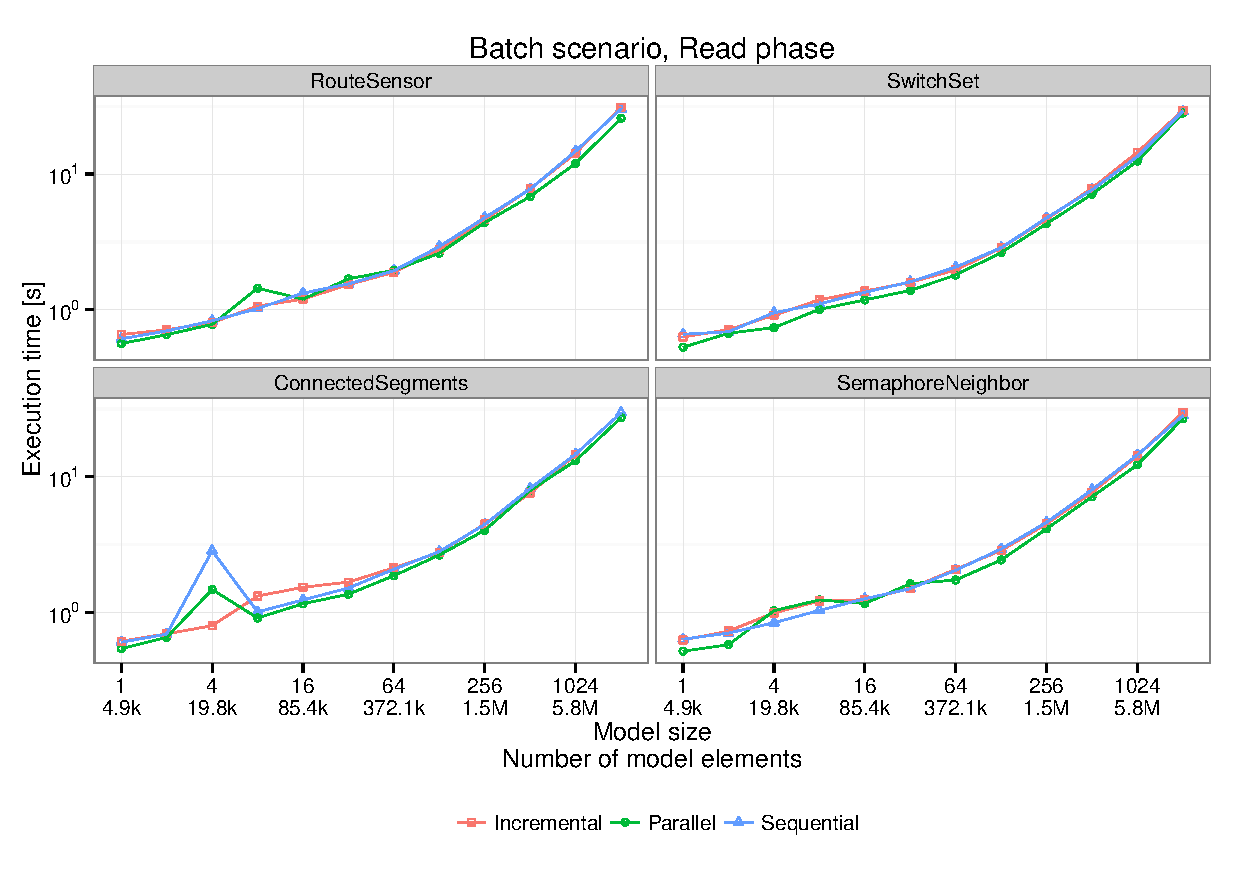
\includegraphics[width=\linewidth]{pdfs/Batch-Read-phase.pdf}
	\vspace{-35pt}
	\captionof{figure}[~Train Benchmark -- Read phase]{Train Benchmark -- Read phase}
	\vspace{10pt}
	\label{fig:tb-measurements-read}
	
	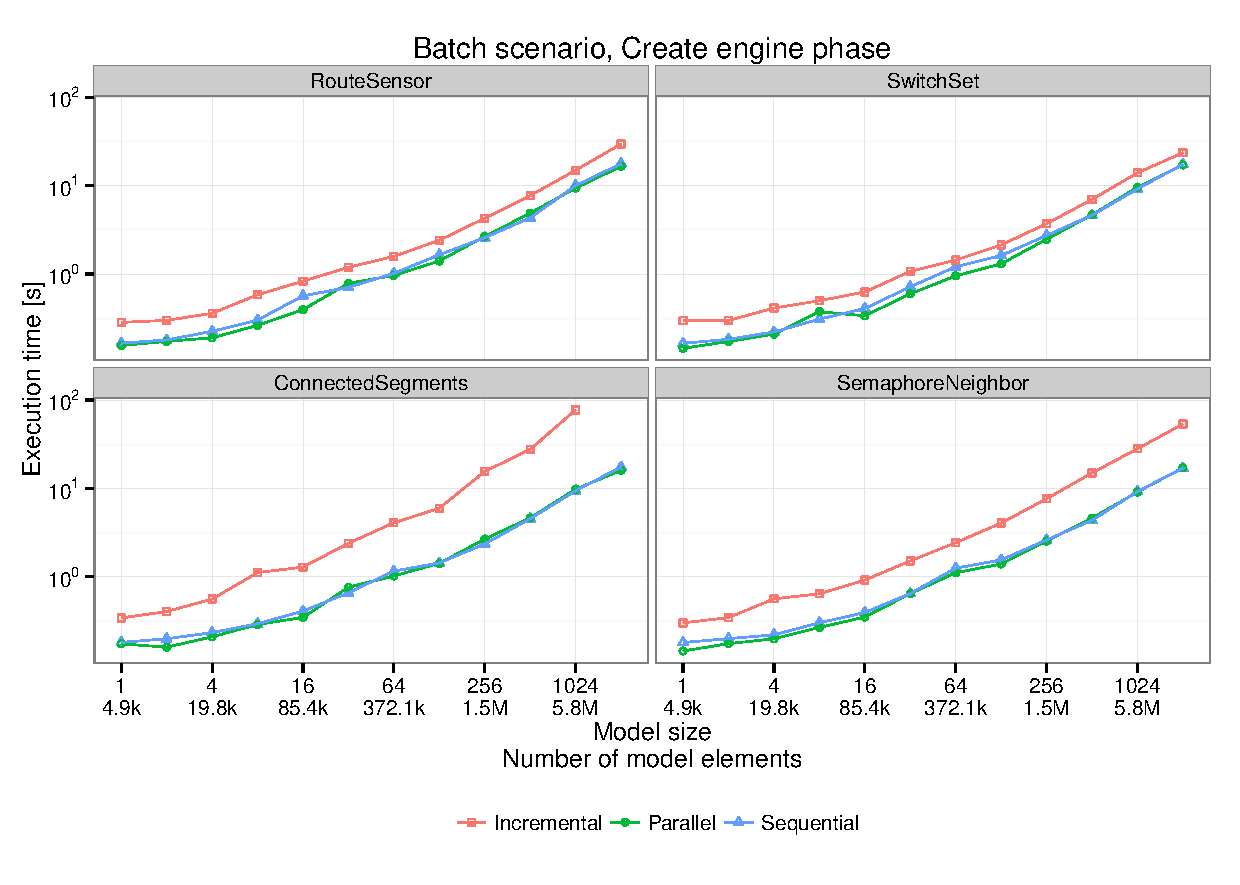
\includegraphics[width=\linewidth]{pdfs/Batch-Create-engine-phase.pdf}
	\vspace{-35pt}
	\captionof{figure}[~Train Benchmark -- Create engine phase]{Train Benchmark -- Create engine phase}
	\vspace{15pt}
	
	\label{fig:tb-measurements-engine}
\end{minipage}

% latex table generated in R 3.2.2 by xtable 1.8-0 package
% Tue Dec 15 23:10:24 2015
\begin{table}[H]
	\centering
	\begin{tabular}{rlrrrrr}
		\hline
		& Case & \shortstack{Model\\scale}  & \shortstack{Calculate\\search plan} & Check & \shortstack{\\Create\\engine} & Read\\ 
		 
		\hline \hline
		1 & ConnectedSegments & 1 & N/A & 0.005 & 0.343 & 0.6160 \\ 
		2 & ConnectedSegments & 2 & N/A & 0.005 & 0.406 & 0.6973 \\ 
		3 & ConnectedSegments & 4 & N/A & 0.006 & 0.561 & 0.8009 \\ 
		4 & ConnectedSegments & 8 & N/A & 0.005 & 1.119 & 1.3233 \\ 
		5 & ConnectedSegments & 16 & N/A & 0.005 & 1.289 & 1.5371 \\ 
		6 & ConnectedSegments & 32 & N/A & 0.006 & 2.402 & 1.6769 \\ 
		7 & ConnectedSegments & 64 & N/A & 0.008 & 4.095 & 2.1386 \\ 
		8 & ConnectedSegments & 128 &  N/A& 0.009 & 5.975 & 2.7748 \\ 
		9 & ConnectedSegments & 256 &  N/A& 0.010 & 15.595 & 4.4905 \\ 
		10 & ConnectedSegments & 512 & N/A & 0.020 & 27.702 & 7.5964 \\ 
		11 & ConnectedSegments & 1024 &N/A  & 0.030 & 77.361 & 14.6564 \\ 
		11 & ConnectedSegments & 2048 & N/A  & - & - & - \\ 
		\hline
		12 & RouteSensor & 1 & N/A & 0.004 & 0.284 & 0.6573 \\ 
		13 & RouteSensor & 2 & N/A & 0.004 & 0.299 & 0.7124 \\ 
		14 & RouteSensor & 4 & N/A & 0.004 & 0.360 & 0.8038 \\ 
		15 & RouteSensor & 8 & N/A & 0.004 & 0.583 & 1.0638 \\ 
		16 & RouteSensor & 16 &N/A  & 0.004 & 0.832 & 1.1981 \\ 
		17 & RouteSensor & 32 &N/A  & 0.004 & 1.192 & 1.5331 \\ 
		18 & RouteSensor & 64 &N/A  & 0.006 & 1.583 & 1.8914 \\ 
		19 & RouteSensor & 128 & N/A & 0.005 & 2.416 & 2.7768 \\ 
		20 & RouteSensor & 256 & N/A & 0.006 & 4.279 & 4.6098 \\ 
		21 & RouteSensor & 512 & N/A & 0.007 & 7.726 & 7.7939 \\ 
		22 & RouteSensor & 1024 &N/A  & 0.009 & 14.953 & 14.2515 \\ 
		23 & RouteSensor & 2048 &N/A  & 0.017 & 29.599 & 31.1415 \\ 
		\hline
		24 & SemaphoreNeighbor & 1 &  N/A& 0.004 & 0.302 & 0.6278 \\ 
		25 & SemaphoreNeighbor & 2 &  N/A& 0.005 & 0.346 & 0.7314 \\ 
		26 & SemaphoreNeighbor & 4 &  N/A& 0.003 & 0.564 & 0.9943 \\ 
		27 & SemaphoreNeighbor & 8 &  N/A& 0.004 & 0.644 & 1.2172 \\ 
		28 & SemaphoreNeighbor & 16 & N/A & 0.005 & 0.920 & 1.2461 \\ 
		29 & SemaphoreNeighbor & 32 & N/A & 0.004 & 1.516 & 1.5093 \\ 
		30 & SemaphoreNeighbor & 64 & N/A & 0.006 & 2.436 & 2.0862 \\ 
		31 & SemaphoreNeighbor & 128 &N/A  & 0.005 & 4.065 & 2.8686 \\ 
		32 & SemaphoreNeighbor & 256 &N/A  & 0.006 & 7.648 & 4.5046 \\ 
		33 & SemaphoreNeighbor & 512 &N/A  & 0.006 & 14.986 & 7.6752 \\ 
		34 & SemaphoreNeighbor & 1024 & N/A & 0.005 & 28.147 & 14.2688 \\ 
		35 & SemaphoreNeighbor & 2048 & N/A & 0.007 & 53.646 & 29.8475 \\ 
		\hline
		36 & SwitchSet & 1 & N/A & 0.004 & 0.298 & 0.6307 \\ 
		37 & SwitchSet & 2 & N/A & 0.004 & 0.299 & 0.7143 \\ 
		38 & SwitchSet & 4 & N/A & 0.004 & 0.413 & 0.9119 \\ 
		39 & SwitchSet & 8 & N/A & 0.004 & 0.500 & 1.1864 \\ 
		40 & SwitchSet & 16 &N/A  & 0.005 & 0.628 & 1.3747 \\ 
		41 & SwitchSet & 32 &N/A  & 0.004 & 1.075 & 1.5935 \\ 
		42 & SwitchSet & 64 &N/A  & 0.005 & 1.439 & 1.9664 \\ 
		43 & SwitchSet & 128 & N/A & 0.006 & 2.134 & 2.8516 \\ 
		44 & SwitchSet & 256 & N/A & 0.007 & 3.714 & 4.6632 \\ 
		45 & SwitchSet & 512 & N/A & 0.009 & 6.989 & 7.8651 \\ 
		46 & SwitchSet & 1024 &N/A  & 0.011 & 13.969 & 14.4903 \\ 
		47 & SwitchSet & 2048 &N/A  & 0.016 & 23.615 & 29.4733 \\ 
		\hline
	\end{tabular}
	\caption{Benchmark results for the incremental algorithm}
	\label{tab:tb-inc}
\end{table}


% latex table generated in R 3.2.2 by xtable 1.8-0 package
% Tue Dec 15 23:21:03 2015
\begin{table}[ht]
	\centering
	\begin{tabular}{rlrrrrr}
				\hline
		& Case & \shortstack{Model\\scale}  & \shortstack{Calculate\\search plan} & Check & \shortstack{\\Create\\engine} & Read\\ 
		\hline
		\hline
		48 & ConnectedSegments & 1 & 0.047 & 0.074 & 0.175 & 0.5428 \\ 
		49 & ConnectedSegments & 2 & 0.043 & 0.037 & 0.160 & 0.6564 \\ 
		50 & ConnectedSegments & 4 & 0.081 & 0.050 & 0.210 & 1.4798 \\ 
		51 & ConnectedSegments & 8 & 0.262 & 0.086 & 0.289 & 0.9131 \\ 
		52 & ConnectedSegments & 16 & 0.396 & 0.128 & 0.348 & 1.1620 \\ 
		53 & ConnectedSegments & 32 & 1.202 & 0.276 & 0.763 & 1.3668 \\ 
		54 & ConnectedSegments & 64 & 2.496 & 0.240 & 1.026 & 1.8711 \\ 
		55 & ConnectedSegments & 128 & 5.115 & 0.341 & 1.423 & 2.6572 \\ 
		56 & ConnectedSegments & 256 & 10.875 & 0.458 & 2.678 & 4.0401 \\ 
		57 & ConnectedSegments & 512 & 14.811 & 1.289 & 4.648 & 7.9337 \\ 
		58 & ConnectedSegments & 1024 & 28.935 & 2.672 & 9.810 & 13.1614 \\ 
		59 & ConnectedSegments & 2048 & 81.477 & 21.778 & 16.030 & 27.3225 \\ 
		\hline
		60 & RouteSensor & 1 & 0.014 & 0.020 & 0.156 & 0.5635 \\ 
		61 & RouteSensor & 2 & 0.019 & 0.024 & 0.173 & 0.6561 \\ 
		62 & RouteSensor & 4 & 0.027 & 0.029 & 0.190 & 0.7796 \\ 
		63 & RouteSensor & 8 & 0.072 & 0.034 & 0.263 & 1.4431 \\ 
		64 & RouteSensor & 16 & 0.119 & 0.045 & 0.396 & 1.1981 \\ 
		65 & RouteSensor & 32 & 0.284 & 0.053 & 0.785 & 1.6905 \\ 
		66 & RouteSensor & 64 & 0.542 & 0.067 & 0.967 & 1.9556 \\ 
		67 & RouteSensor & 128 & 1.207 & 0.104 & 1.406 & 2.6108 \\ 
		68 & RouteSensor & 256 & 2.539 & 0.151 & 2.669 & 4.3887 \\ 
		69 & RouteSensor & 512 & 3.800 & 0.189 & 4.885 & 6.8383 \\ 
		70 & RouteSensor & 1024 & 7.025 & 0.285 & 9.403 & 11.9807 \\ 
		71 & RouteSensor & 2048 & 14.836 & 0.380 & 16.569 & 25.7272 \\ 
		\hline
		72 & SemaphoreNeighbor & 1 & 0.024 & 0.040 & 0.145 & 0.5200 \\ 
		73 & SemaphoreNeighbor & 2 & 0.041 & 0.052 & 0.176 & 0.5795 \\ 
		74 & SemaphoreNeighbor & 4 & 0.066 & 0.083 & 0.199 & 1.0330 \\ 
		75 & SemaphoreNeighbor & 8 & 0.103 & 0.050 & 0.268 & 1.2399 \\ 
		76 & SemaphoreNeighbor & 16 & 0.210 & 0.195 & 0.351 & 1.1655 \\ 
		77 & SemaphoreNeighbor & 32 & 0.702 & 0.231 & 0.646 & 1.6327 \\ 
		78 & SemaphoreNeighbor & 64 & 1.534 & 0.422 & 1.113 & 1.7387 \\ 
		79 & SemaphoreNeighbor & 128 & 2.776 & 0.123 & 1.400 & 2.4430 \\ 
		80 & SemaphoreNeighbor & 256 & 5.743 & 1.732 & 2.543 & 4.1405 \\ 
		81 & SemaphoreNeighbor & 512 & 7.488 & 0.250 & 4.615 & 7.1392 \\ 
		82 & SemaphoreNeighbor & 1024 & 15.876 & 1.702 & 9.112 & 12.2774 \\ 
		83 & SemaphoreNeighbor & 2048 & 52.981 & 0.665 & 17.138 & 26.8228 \\ 
		\hline
		84 & SwitchSet & 1 & 0.019 & 0.011 & 0.145 & 0.5297 \\ 
		85 & SwitchSet & 2 & 0.025 & 0.017 & 0.173 & 0.6714 \\ 
		86 & SwitchSet & 4 & 0.028 & 0.021 & 0.209 & 0.7397 \\ 
		87 & SwitchSet & 8 & 0.037 & 0.028 & 0.375 & 1.0071 \\ 
		88 & SwitchSet & 16 & 0.064 & 0.027 & 0.337 & 1.1823 \\ 
		89 & SwitchSet & 32 & 0.230 & 0.025 & 0.599 & 1.3891 \\ 
		90 & SwitchSet & 64 & 0.497 & 0.047 & 0.954 & 1.8049 \\ 
		91 & SwitchSet & 128 & 0.895 & 0.038 & 1.307 & 2.6413 \\ 
		92 & SwitchSet & 256 & 2.009 & 0.069 & 2.480 & 4.3071 \\ 
		93 & SwitchSet & 512 & 2.885 & 0.084 & 4.675 & 7.1133 \\ 
		94 & SwitchSet & 1024 & 6.073 & 0.131 & 9.606 & 12.4735 \\ 
		95 & SwitchSet & 2048 & 11.590 & 0.148 & 17.169 & 28.1495 \\ 
		\hline
	\end{tabular}
	\caption{Benchmark result for the sequential local search-based algorithm}
		\label{tab:tb-seq}
\end{table}


% latex table generated in R 3.2.2 by xtable 1.8-0 package
% Tue Dec 15 23:40:09 2015
\begin{table}[ht]
	\centering
	\begin{tabular}{rlrrrrr}
		\hline
		& Case & \shortstack{Model\\scale}  & \shortstack{Calculate\\search plan} & Check & \shortstack{\\Create\\engine} & Read\\ 
		\hline
		\hline
		96 & ConnectedSegments & 1 & 0.160 & 0.029 & 0.182 & 0.6048 \\ 
		97 & ConnectedSegments & 2 & 0.179 & 0.041 & 0.200 & 0.6937 \\ 
		98 & ConnectedSegments & 4 & 0.240 & 0.069 & 0.234 & 2.8547 \\ 
		99 & ConnectedSegments & 8 & 0.455 & 0.079 & 0.295 & 1.0115 \\ 
		100 & ConnectedSegments & 16 & 0.859 & 0.247 & 0.411 & 1.2394 \\ 
		101 & ConnectedSegments & 32 & 2.020 & 0.258 & 0.661 & 1.5176 \\ 
		102 & ConnectedSegments & 64 & 3.175 & 0.735 & 1.162 & 2.0864 \\ 
		103 & ConnectedSegments & 128 & 6.631 & 0.827 & 1.438 & 2.8166 \\ 
		104 & ConnectedSegments & 256 & 14.495 & 3.906 & 2.361 & 4.4578 \\ 
		105 & ConnectedSegments & 512 & 20.719 & 3.109 & 4.542 & 8.2206 \\ 
		106 & ConnectedSegments & 1024 & 39.900 & 6.585 & 9.425 & 14.7102 \\ 
		107 & ConnectedSegments & 2048 & 104.046 & 34.750 & 17.492 & 29.6772 \\
		\hline
		108 & RouteSensor & 1 & 0.092 & 0.006 & 0.165 & 0.6108 \\ 
		109 & RouteSensor & 2 & 0.104 & 0.009 & 0.180 & 0.6993 \\ 
		110 & RouteSensor & 4 & 0.147 & 0.014 & 0.225 & 0.8292 \\ 
		111 & RouteSensor & 8 & 0.265 & 0.023 & 0.302 & 1.0207 \\ 
		112 & RouteSensor & 16 & 0.471 & 0.034 & 0.567 & 1.3270 \\ 
		113 & RouteSensor & 32 & 0.795 & 0.060 & 0.708 & 1.5513 \\ 
		114 & RouteSensor & 64 & 1.398 & 0.067 & 1.019 & 1.9423 \\ 
		115 & RouteSensor & 128 & 2.529 & 0.102 & 1.655 & 2.9249 \\ 
		116 & RouteSensor & 256 & 5.121 & 0.174 & 2.583 & 4.7742 \\ 
		117 & RouteSensor & 512 & 10.334 & 0.227 & 4.330 & 7.7517 \\ 
		118 & RouteSensor & 1024 & 19.039 & 0.488 & 10.023 & 14.7573 \\ 
		119 & RouteSensor & 2048 & 38.614 & 0.525 & 17.730 & 30.2251 \\ 
		\hline
		120 & SemaphoreNeighbor & 1 & 0.138 & 0.036 & 0.181 & 0.6367 \\ 
		121 & SemaphoreNeighbor & 2 & 0.152 & 0.060 & 0.200 & 0.7069 \\ 
		122 & SemaphoreNeighbor & 4 & 0.206 & 0.100 & 0.221 & 0.8413 \\ 
		123 & SemaphoreNeighbor & 8 & 0.353 & 0.084 & 0.302 & 1.0385 \\ 
		124 & SemaphoreNeighbor & 16 & 0.663 & 0.133 & 0.395 & 1.2638 \\ 
		125 & SemaphoreNeighbor & 32 & 1.355 & 0.356 & 0.648 & 1.5020 \\ 
		126 & SemaphoreNeighbor & 64 & 1.993 & 0.287 & 1.254 & 2.0495 \\ 
		127 & SemaphoreNeighbor & 128 & 4.037 & 0.957 & 1.554 & 2.9425 \\ 
		128 & SemaphoreNeighbor & 256 & 8.168 & 0.994 & 2.621 & 4.6234 \\ 
		129 & SemaphoreNeighbor & 512 & 14.477 & 2.945 & 4.356 & 8.0286 \\ 
		130 & SemaphoreNeighbor & 1024 & 27.131 & 6.580 & 9.242 & 14.5130 \\ 
		131 & SemaphoreNeighbor & 2048 & 52.988 & 44.576 & 17.004 & 28.2886 \\ 
		\hline
		132 & SwitchSet & 1 & 0.105 & 0.004 & 0.165 & 0.6604 \\ 
		133 & SwitchSet & 2 & 0.113 & 0.005 & 0.183 & 0.6893 \\ 
		134 & SwitchSet & 4 & 0.151 & 0.009 & 0.222 & 0.9518 \\ 
		135 & SwitchSet & 8 & 0.232 & 0.010 & 0.309 & 1.1063 \\ 
		136 & SwitchSet & 16 & 0.354 & 0.014 & 0.408 & 1.3451 \\ 
		137 & SwitchSet & 32 & 0.736 & 0.025 & 0.718 & 1.6062 \\ 
		138 & SwitchSet & 64 & 1.044 & 0.033 & 1.211 & 2.0653 \\ 
		139 & SwitchSet & 128 & 2.188 & 0.056 & 1.622 & 2.8650 \\ 
		140 & SwitchSet & 256 & 5.262 & 0.093 & 2.735 & 4.7560 \\ 
		141 & SwitchSet & 512 & 9.661 & 0.132 & 4.624 & 7.6547 \\ 
		142 & SwitchSet & 1024 & 18.099 & 0.142 & 9.202 & 13.4744 \\ 
		143 & SwitchSet & 2048 & 34.605 & 0.262 & 17.445 & 29.0464 \\ 
		\hline
	\end{tabular}
	\caption{Benchmark result for the parallel local search-based algorithm}
	\label{tab:tb-par}		
\end{table}

%\label{page:last}
\end{document}
